%%%%%%%%%%%%%%%%%%%%%%%%%%%%%%%%%%%%%%%%%
% Classicthesis Typographic Thesis
% LaTeX Template
% Version 1.4 (1/1/16)
%
% This template has been downloaded from:
% http://www.LaTeXTemplates.com
%
% Original author:
% André Miede (http://www.miede.de) with commenting modifications by:
% Vel (vel@LaTeXTemplates.com)
%
% License:
% GNU General Public License (v2)
%
% General Tips:
% 1) Make sure to edit the classicthesis-config.file
% 2) New enumeration (A., B., C., etc in small caps): \begin{aenumerate} \end{aenumerate}
% 3) For margin notes: \marginpar or \graffito{}
% 4) Do not use bold fonts in this style, it is designed around them
% 5) Use tables as in the examples
% 6) See classicthesis-preamble.sty for useful commands
%
%%%%%%%%%%%%%%%%%%%%%%%%%%%%%%%%%%%%%%%%%

%----------------------------------------------------------------------------------------
%	PACKAGES AND OTHER DOCUMENT CONFIGURATIONS
%----------------------------------------------------------------------------------------

\documentclass[
  oneside,openright,titlepage,numbers=noenddot,headinclude,%1headlines,
  footinclude=true,cleardoublepage=empty,
  obeyspaces,
  dottedtoc, % Make page numbers in the table of contents flushed right with dots leading to them
  BCOR=5mm,paper=a4,fontsize=11pt, % Binding correction, paper type and font size
  ngerman,american, % Languages, change this to your language(s)
  ]{scrreprt} 
              
% Includes the file which contains all the document configurations and packages - make sure to edit this file
%%%%%%%%%%%%%%%%%%%%%%%%%%%%%%%%%%%%%%%%%
% Classicthesis Typographic Thesis
% Configuration File
%
% This file has been downloaded from:
% http://www.LaTeXTemplates.com
%
% Original author:
% André Miede (http://www.miede.de) with extensive commenting changes by:
% Vel (vel@LaTeXTemplates.com)
%
% License:
% GNU General Public License (v2)
%
% Important note:
% The main lines to change in this file are in the DOCUMENT VARIABLES
% section, the rest of the file is for advanced configuration.
%
%%%%%%%%%%%%%%%%%%%%%%%%%%%%%%%%%%%%%%%%%

%----------------------------------------------------------------------------------------
%	CHARACTER ENCODING
%----------------------------------------------------------------------------------------

\PassOptionsToPackage{utf8}{inputenc} % Set the encoding of your files. UTF-8 is the only sensible encoding nowadays. If you can't read äöüßáéçèê∂åëæƒÏ€ then change the encoding setting in your editor, not the line below. If your editor does not support utf8 use another editor!
\usepackage{inputenc}

%----------------------------------------------------------------------------------------
%	DOCUMENT VARIABLES
%	Fill in the lines below to enter your information into the thesis template
%	Each of the commands can be cited anywhere in the thesis
%----------------------------------------------------------------------------------------

% Remove drafting to get rid of the '[ Date - classicthesis version 4.0 ]' text at the bottom of every page
\PassOptionsToPackage{eulerchapternumbers,listings,drafting, pdfspacing, subfig,beramono,eulermath,parts}{classicthesis}
% Available options: drafting parts nochapters linedheaders eulerchapternumbers beramono eulermath pdfspacing minionprospacing tocaligned dottedtoc manychapters listings floatperchapter subfig

\newcommand{\myTitle}{Simultaneous Localization and Mapping in Lightweight Autonomous Vehicles\xspace}
\newcommand{\mySubtitle}{Application of autonomous vehicle techniques in low-cost light electric platforms\xspace}
\newcommand{\myDegree}{Master of Science in Mechanical Engineering (Ing.)\xspace}
\newcommand{\myName}{Yago Lizarribar Carrillo\xspace}
\newcommand{\myProf}{Jorge Juan Gil\xspace}
% \newcommand{\myOtherProf}{Put name here\xspace}
\newcommand{\mySupervisor}{Kent Larson\xspace}
\newcommand{\myOtherSupervisor}{Michael Lin\xspace}
% \newcommand{\myDepartment}{Put data here\xspace}
\newcommand{\myUni}{Tecnun--University of Navarra\xspace}
\newcommand{\myLocation}{San Sebastian\xspace}
\newcommand{\myTime}{July 2018\xspace}
\newcommand{\myVersion}{version 1.0\xspace}

%----------------------------------------------------------------------------------------
%	USEFUL COMMANDS
%----------------------------------------------------------------------------------------

\newcommand{\ie}{i.\,e.}
\newcommand{\Ie}{I.\,e.}
\newcommand{\eg}{e.\,g.}
\newcommand{\Eg}{E.\,g.} 
\newcommand{\parunder}[1]{\paragraph{\underline{#1}}\graffito{\textsc{#1}}}
\newcommand{\arrow}{$\,\to\,$}
\providecommand{\keywords}[1]
{
  \small	
  \textbf{\textit{Keywords---}} #1
}
\providecommand{\keywordsesp}[1]
{
  \small	
  \textbf{\textit{Palabras clave---}} #1
}

\newcounter{dummy} % Necessary for correct hyperlinks (to index, bib, etc.)
\providecommand{\mLyX}{L\kern-.1667em\lower.25em\hbox{Y}\kern-.125emX\@}
\newlength{\abcd} % for ab..z string length calculation

%----------------------------------------------------------------------------------------
%	PACKAGES
%----------------------------------------------------------------------------------------

\usepackage{lipsum} % Used for inserting dummy 'Lorem ipsum' text into the template

%------------------------------------------------

%\PassOptionsToPackage{ngerman,american}{babel}  % Change this to your language(s)
% Spanish languages need extra options in order to work with this template
%\PassOptionsToPackage{spanish,es-lcroman}{babel}
\usepackage{babel}

%------------------------------------------------			

\usepackage{csquotes}
% \PassOptionsToPackage{%
% %backend=biber, % Instead of bibtex
% backend=bibtex8,bibencoding=ascii,%
% language=auto,%
% style=numeric-comp,%
% %style=authoryear-comp, % Author 1999, 2010
% %bibstyle=authoryear,dashed=false, % dashed: substitute rep. author with ---
% sorting=nyt, % name, year, title
% maxbibnames=10, % default: 3, et al.
% %backref=true,%
% natbib=true % natbib compatibility mode (\citep and \citet still work)
% }{biblatex}
% \usepackage{biblatex}
\usepackage{multibib}

% This is for changing chapter to section in bibliography
% \usepackage{tocbibind}
 
 %------------------------------------------------

% \PassOptionsToPackage{fleqn}{amsmath} % Math environments and more by the AMS 
 \usepackage{amsmath}
 
 %------------------------------------------------

\PassOptionsToPackage{T1}{fontenc} % T2A for cyrillics
\usepackage{fontenc}

%------------------------------------------------

\usepackage{textcomp} % Fix warning with missing font shapes

%------------------------------------------------

\usepackage{scrhack} % Fix warnings when using KOMA with listings package  

%------------------------------------------------

\usepackage{xspace} % To get the spacing after macros right

%------------------------------------------------

\usepackage{mparhack} % To get marginpar right

%------------------------------------------------

\usepackage{fixltx2e} % Fixes some LaTeX stuff 

%------------------------------------------------

\usepackage[inline]{enumitem} % Inline lists

%------------------------------------------------

\usepackage{longtable} % Long tables

%------------------------------------------------

\PassOptionsToPackage{smaller}{acronym} % Include printonlyused in the first bracket to only show acronyms used in the text
\usepackage{acronym} % Nice macros for handling all acronyms in the thesis

%\renewcommand*{\acsfont}[1]{\textssc{#1}} % For MinionPro
\renewcommand*{\aclabelfont}[1]{\acsfont{#1}}

%------------------------------------------------

\PassOptionsToPackage{pdftex}{graphicx}
\usepackage{graphicx} 

%----------------------------------------------------------------------------------------
%	FLOATS: TABLES, FIGURES AND CAPTIONS SETUP
%----------------------------------------------------------------------------------------

\usepackage{tabularx} % Better tables
\setlength{\extrarowheight}{3pt} % Increase table row height
\newcommand{\tableheadline}[1]{\multicolumn{1}{c}{\spacedlowsmallcaps{#1}}}
\newcommand{\myfloatalign}{\centering} % To be used with each float for alignment
\usepackage{caption}
\captionsetup{font=small}
\usepackage{subfig}  

%----------------------------------------------------------------------------------------
%	CODE LISTINGS SETUP
%----------------------------------------------------------------------------------------

\usepackage{listings} 
%\lstset{emph={trueIndex,root},emphstyle=\color{BlueViolet}}%\underbar} % For special keywords
\lstset{language=[LaTeX]Tex,%C++ % Specify the language(s) for listings here
morekeywords={PassOptionsToPackage,selectlanguage},
keywordstyle=\color{RoyalBlue}, % Add \bfseries for bold
basicstyle=\small\ttfamily, % Makes listings a smaller font size and a different font
%identifierstyle=\color{NavyBlue}, % Color of text inside brackets
commentstyle=\color{Green}\ttfamily, % Color of comments
stringstyle=\rmfamily, % Font type to use for strings
numbers=left, % Change left to none to remove line numbers
numberstyle=\scriptsize, % Font size of the line numbers
stepnumber=5, % Increment of line numbers
numbersep=8pt, % Distance of line numbers from code listing
showstringspaces=false, % Sets whether spaces in strings should appear underlined
breaklines=true, % Force the code to stay in the confines of the listing box
%frameround=ftff, % Uncomment for rounded frame
%frame=single, % Frame border - none/leftline/topline/bottomline/lines/single/shadowbox/L
belowcaptionskip=.75\baselineskip % Space after the "Listing #: Desciption" text and the listing box
}

%----------------------------------------------------------------------------------------
%	HYPERREFERENCES
%----------------------------------------------------------------------------------------
\PassOptionsToPackage{hyphens}{url}
\PassOptionsToPackage{pdftex,hyperfootnotes=false,pdfpagelabels}{hyperref}
\usepackage{hyperref}  % backref linktocpage pagebackref
\pdfcompresslevel=9
\pdfadjustspacing=1

\hypersetup{
% Uncomment the line below to remove all links (to references, figures, tables, etc), useful for b/w printouts
%draft, 
colorlinks=true, linktocpage=true, pdfstartpage=3, pdfstartview=FitV,
% Uncomment the line below if you want to have black links (e.g. for printing black and white)
%colorlinks=false, linktocpage=false, pdfborder={0 0 0}, pdfstartpage=3, pdfstartview=FitV, 
breaklinks=true, pdfpagemode=UseNone, pageanchor=true, pdfpagemode=UseOutlines,%
plainpages=false, bookmarksnumbered, bookmarksopen=true, bookmarksopenlevel=1,%
hypertexnames=true, pdfhighlight=/O,%nesting=true,%frenchlinks,%
urlcolor=webbrown, linkcolor=RoyalBlue, citecolor=webgreen, %pagecolor=RoyalBlue,%
    %urlcolor=Black, linkcolor=Black, citecolor=Black, %pagecolor=Black,%
%------------------------------------------------
% PDF file meta-information
pdftitle={\myTitle},
pdfauthor={\textcopyright\ \myName},
pdfsubject={Autonomous Vehicles},
pdfkeywords={autonomous, cities, slam, medialab, cityscience},
pdfcreator={pdfLaTeX},
pdfproducer={LaTeX with hyperref and classicthesis}
%------------------------------------------------
}

%----------------------------------------------------------------------------------------
%	AUTOREFERENCES SETUP
%	Redefines how references in text are prefaced for different 
%	languages (e.g. "Section 1.2" or "section 1.2")
%----------------------------------------------------------------------------------------

\makeatletter
\@ifpackageloaded{babel}
{
\addto\extrasamerican{
\renewcommand*{\figureautorefname}{Figure}
\renewcommand*{\tableautorefname}{Table}
\renewcommand*{\partautorefname}{Part}
\renewcommand*{\chapterautorefname}{Chapter}
\renewcommand*{\sectionautorefname}{Section}
\renewcommand*{\subsectionautorefname}{Section}
\renewcommand*{\subsubsectionautorefname}{Section}
}
\addto\extrasngerman{
\renewcommand*{\paragraphautorefname}{Absatz}
\renewcommand*{\subparagraphautorefname}{Unterabsatz}
\renewcommand*{\footnoteautorefname}{Fu\"snote}
\renewcommand*{\FancyVerbLineautorefname}{Zeile}
\renewcommand*{\theoremautorefname}{Theorem}
\renewcommand*{\appendixautorefname}{Anhang}
\renewcommand*{\equationautorefname}{Gleichung}
\renewcommand*{\itemautorefname}{Punkt}
}
\providecommand{\subfigureautorefname}{\figureautorefname} % Fix to getting autorefs for subfigures right
}{\relax}
\makeatother

%----------------------------------------------------------------------------------------

\usepackage{classicthesis/classicthesis} 

%----------------------------------------------------------------------------------------
% Avoid error of I/O
\usepackage{morewrites}

%----------------------------------------------------------------------------------------

\usepackage{pdfpages}

%----------------------------------------------------------------------------------------
%	CHANGING TEXT AREA 
%----------------------------------------------------------------------------------------

\linespread{1.05} % a bit more for Palatino
\areaset[current]{360pt}{760pt} % 686 (factor 2.2) + 33 head + 42 head \the\footskip
\setlength{\marginparwidth}{7em}%
\setlength{\marginparsep}{2em}%
\setlength{\parskip}{.5em}

\setlength\parindent{0pt}

%----------------------------------------------------------------------------------------
%	USING DIFFERENT FONTS
%----------------------------------------------------------------------------------------

%\usepackage[oldstylenums]{kpfonts} % oldstyle notextcomp
%\usepackage[osf]{libertine}
%\usepackage[light,condensed,math]{iwona}
%\renewcommand{\sfdefault}{iwona}
%\usepackage{lmodern} % <-- no osf support :-(
%\usepackage{cfr-lm} % 
%\usepackage[urw-garamond]{mathdesign} <-- no osf support :-(
%\usepackage[default,osfigures]{opensans} % scale=0.95 
%\usepackage[sfdefault]{FiraSans}

\newcites{intro}{Chapter 01}
\newcites{auton}{Chapter 02}
\newcites{slam}{Chapter 03}
% \newcites{nexus}{Chapter 04}
\newcites{pev}{Chapter 05}
% \newcites{budget}{Chapter 06}
% \newcites{concl}{Chapter 07}


%\hyphenation{Put special hyphenation here}

\begin{document}

\frenchspacing % Reduces space after periods to make text more compact

\raggedbottom % Makes all pages the height of the text on that page

\selectlanguage{american} % Select your default language - e.g. american or ngerman

\pagenumbering{roman} % Roman page numbering prior to the start of the thesis content (i, ii, iii, etc)

\pagestyle{plain} % Suppress headers for the pre-content pages

%----------------------------------------------------------------------------------------
%	PRE-CONTENT THESIS PAGES
%----------------------------------------------------------------------------------------

% Title Page

\begin{titlepage}

% \begin{addmargin}[-1cm]{-3cm} % For twoside
\begin{addmargin}[-1cm]{-1cm}
\begin{center}
\large

\hfill
\vfill

\begingroup
\color{Maroon}\spacedallcaps{\myTitle} \\ \bigskip % Thesis title
\endgroup

\spacedlowsmallcaps{\myName} % Your name

\vfill

\begin{figure}[h!]
  \centering
  \subfloat{
\includegraphics[width=6cm]{pictures/tecnun.png}} \hspace*{\fill}
  \subfloat{
\includegraphics[width=5cm]{pictures/medialab.png}}
\end{figure} \medskip % Picture

\mySubtitle \\ \medskip % Thesis subtitle
\myDegree \\
%\myDepartment \\
%\myFaculty \\
\myUni \\ \bigskip

\myTime\ -- \myVersion % Time and version

\vfill

\end{center}
\end{addmargin}

\end{titlepage} % Main title page

% Back of the title page

\thispagestyle{empty}

\hfill

\vfill

\noindent\myName: \textit{\myTitle,} \mySubtitle, %\myDegree, 
\textcopyright\ \myTime

% You may wish to do something with the back of the title page, such as including your supervisors, location or time frame of the work. Below is an example of doing so although you may want to tweak it to your liking.

%\bigskip

%\noindent\spacedlowsmallcaps{Supervisors}: \\
%\myProf \\
%\myOtherProf \\ 
%\mySupervisor

%\medskip \\

%\noindent\spacedlowsmallcaps{Location}: \\
%\myLocation

%\medskip \\

%\noindent\spacedlowsmallcaps{Time Frame}: \\
%\myTime
 % Back of the title page

\cleardoublepage% Abstract

%\renewcommand{\abstractname}{Abstract} % Uncomment to change the name of the abstract

\pdfbookmark[1]{Abstract}{Abstract} % Bookmark name visible in a PDF viewer

\begingroup
\let\clearpage\relax
\let\cleardoublepage\relax
\let\cleardoublepage\relax

\chapter*{Abstract}
\textbf{Self--driving vehicles} will be a reality in the not so distant future of cities. Much of the attention today is focused on cars, although they face great challenges in years to come before their implementation, thus creating an ample spot for lightweight alternatives to blossom. This thesis is about one of those alternatives, the \textbf{Persuasive Electric Vehicle}, and the approaches taken to overcome the problems autonomous vehicles have. Specially interesting is the problem of \textbf{Simultaneous Localization and Mapping} due to its complexity and possibilities it opens to achieve fully autonomous platforms. In the chapters that follow, the reader will find how it was tackled, what are the results employing different techniques and how it could be improved so that autonomous lightweight vehicles can start to be seen on the streets of our cities.\bigskip

\keywords{Autonomous Vehicles, Cities, Lightweight platforms, Shared Mobility, Simultaneous Localization and Mapping}

\endgroup			

\vfill % Abstract page

\cleardoublepage% Abstract

%\renewcommand{\abstractname}{Abstract} % Uncomment to change the name of the abstract

\pdfbookmark[1]{Abstract [Spanish]}{Abstract [Spanish]} % Bookmark name visible in a PDF viewer

\begingroup
\let\clearpage\relax
\let\cleardoublepage\relax
\let\cleardoublepage\relax

\chapter*{Resumen}
Los \textbf{veh\'iculos auton\'omos} ser\'an parte de la realidad de las ciudades en un futuro no muy lejano. La mayor parte de la atenci\'on est\'a fijada en los coches, aunque deber\'an superar una gran cantidad obst\'aculos antes de ocupar las urbes, dejando un espacio de crecimiento para otras alternativas. Esta tesis es sobre una de esas alternativas, el \textbf{Persuasive Electric Vehicle}, y las metodolog\'ias implementadas para superar dichos obst\'aculos. Especialmente interesante es el problema de la \textbf{Localizaci\'on Simult\'anea y Mapeado} debido a su complejidad y las posibilidades que abre para el desarrollo de plataformas completamente auton\'onomas. En los siguientes cap\'itulos, el lector aprender\'a como se ha afrontado dicho problema, cu\'ales son los resultados empleando diferentes t\'ecnicas y qu\'e aspectos se deber\'ia reforzar para ver en el futuro veh\'iculos aut\'onomos ligeros circular por las ciudades del mundo. 

\keywordsesp{Veh\'iculos Aut\'onomos, Ciudades, Plataformas Ligeras, Movilidad compartida, Localizaci\'on Simult\'anea y Mapeado}

\endgroup			

\vfill % Abstract page in Spanish

\cleardoublepage% Acknowledgements

\pdfbookmark[1]{Acknowledgements}{Acknowledgements} % Bookmark name visible in a PDF viewer

\begin{flushright}{\slshape    
In other words, the rule about great scientific advances is that to \\ 
make them you have to break the rules. Nobody has ever won a Nobel Prize \\ 
doing what they’re told, or even by following someone else’s blueprints.} \\ \medskip
---{Joichi Ito, Director of the MIT Media Lab}
\end{flushright}

\bigskip

% “In other words, the rule about great scientific advances is that to  by  In” 
% ― Joichi Ito, Whiplash: How to Survive Our Faster Future

%----------------------------------------------------------------------------------------

\begingroup

\let\clearpage\relax
\let\cleardoublepage\relax
\let\cleardoublepage\relax

\chapter*{Acknowledgements}

First of all, thank you \textbf{Kent Larson} for this amazing opportunity. Your decision of letting me in the City Science group opened my eyes and showed me worlds that I could not even imagine. \bigskip

I am enormously grateful to \textbf{Michael}, \textbf{Abhishek} and \textbf{Phil} for their leadership of the mobility team and for taking me in without hesitation. Thanks to \textbf{Jerry} for all these months full of great moments and hard work side by side until very late hours. To \textbf{Justin, Luke} for all those lessons and and fun moments. To my Taiwanese family \textbf{Ting--Kai and Frank} for teaching me, for helping me and for welcoming me in your wonderful country.\bigskip

To \textbf{Luis} and \textbf{Azucena} for all the invaluable help these months, for all those pieces of advice, for everything in general. And this gratefulness is extended to the whole City Science family: \textbf{Ana, Andr\'es, Ariel, Arnaud, Carson, Chrisoula, Jason, Laya, Lucas, Maggie, Markus, Mary, Nina, Roonan, Ryan, Thomas and Yasushi}. \bigskip

To \textbf{Jose} and \textbf{Eduardo}, for those great talks about every subject imaginable and lessons to become a better researcher.\bigskip

Many thanks to \textbf{Tecnun} for nominating me to go to these amazing place and all those professors that throughout these 6 years have inspired me and helped me become a better engineer and person. \bigskip

To my family, my parents, my friends here and there, for their support both emotional and finantial. And specially to you, \textbf{I}...\bigskip

\textsc{Thank you All!}
\endgroup % Acknowledgements page

\pagestyle{scrheadings} % Show chapter titles as headings

\cleardoublepage% Table of Contents - List of Tables/Figures/Listings and Acronyms

\refstepcounter{dummy}

\pdfbookmark[1]{\contentsname}{tableofcontents} % Bookmark name visible in a PDF viewer

\setcounter{tocdepth}{1} % Depth of sections to include in the table of contents - currently up to subsections

\setcounter{secnumdepth}{3} % Depth of sections to number in the text itself - currently up to subsubsections

\manualmark
\markboth{\spacedlowsmallcaps{\contentsname}}{\spacedlowsmallcaps{\contentsname}}
\tableofcontents 
\automark[section]{chapter}
\renewcommand{\chaptermark}[1]{\markboth{\spacedlowsmallcaps{#1}}{\spacedlowsmallcaps{#1}}}
\renewcommand{\sectionmark}[1]{\markright{\thesection\enspace\spacedlowsmallcaps{#1}}}

\clearpage

\begingroup 
\let\clearpage\relax
\let\cleardoublepage\relax
\let\cleardoublepage\relax

%----------------------------------------------------------------------------------------
%	List of Figures
%----------------------------------------------------------------------------------------

\refstepcounter{dummy}
%\addcontentsline{toc}{chapter}{\listfigurename} % Uncomment if you would like the list of figures to appear in the table of contents
\pdfbookmark[1]{\listfigurename}{lof} % Bookmark name visible in a PDF viewer

\listoffigures

\vspace{8ex}
\newpage

%----------------------------------------------------------------------------------------
%	List of Tables
%----------------------------------------------------------------------------------------

\refstepcounter{dummy}
%\addcontentsline{toc}{chapter}{\listtablename} % Uncomment if you would like the list of tables to appear in the table of contents
\pdfbookmark[1]{\listtablename}{lot} % Bookmark name visible in a PDF viewer

\listoftables
        
\vspace{8ex}
\newpage
    
%----------------------------------------------------------------------------------------
%	List of Listings
%---------------------------------------------------------------------------------------- 

\refstepcounter{dummy}
%\addcontentsline{toc}{chapter}{\lstlistlistingname} % Uncomment if you would like the list of listings to appear in the table of contents
\pdfbookmark[1]{\lstlistlistingname}{lol} % Bookmark name visible in a PDF viewer

\lstlistoflistings 

\vspace{8ex}
\newpage
       
%----------------------------------------------------------------------------------------
%	Acronyms
%----------------------------------------------------------------------------------------

\refstepcounter{dummy}
%\addcontentsline{toc}{chapter}{Acronyms} % Uncomment if you would like the acronyms to appear in the table of contents
\pdfbookmark[1]{Acronyms}{acronyms} % Bookmark name visible in a PDF viewer

\markboth{\spacedlowsmallcaps{Acronyms}}{\spacedlowsmallcaps{Acronyms}}

\chapter*{Acronyms}

\begin{acronym}[DARPA]
\acro{AI}{Artificial Intelligence}
\acro{API}{Application Programming Interface}
\acro{AV}{Autonomous Vehicle}
\acro{CS}{City Science}
\acro{CV}{Computer Vision}
\acro{DARPA}{Defense Advanced Research Projects Agency}
\acro{DWA}{Dynamic Window Approach}
\acro{EKF}{Extended Kalman Filter}
\acro{GPS}{Global Positioning System}
\acro{GPU}{Graphics Processing Unit}
\acro{ICP}{Iterative Closest Point}
\acro{IMU}{Inertial Measurement Unit}
\acro{LIDAR}{Light Detection and Ranging}
\acro{MDP}{Markov Decision Process}
\acro{ML}{Media Lab}
\acro{NDT}{Normal Distributions Transform}
\acro{PEV}{Persuasive Electric Vehicle}
\acro{ROS}{Robot Operating System}
\acro{RTK}{Real Time Kinematics}
\acro{SAV}{Shared Autonomous Vehicle}
\acro{SLAM}{Simultaneous Localization and Mapping}
\acro{TAF}{Taipei Air Force}
\acro{UKF}{Unscented Kalman Filter}
\acro{VMT}{Vehicle-Miles Travelled}
\end{acronym}  
                   
\endgroup % Contents, list of figures/tables/listings and acronyms

\cleardoublepage

\pagenumbering{arabic} % Arabic page numbering for thesis content (1, 2, 3, etc)

\cleardoublepage % Avoids problems with pdfbookmark

% %----------------------------------------------------------------------------------------
% %	THESIS CONTENT - CHAPTERS
% %----------------------------------------------------------------------------------------

% Introduction chapter to the topic

\chapter{Introduction}
\label{ch:intro}

This chapter will give a justification for the Persuasive Electric Vehicle (PEV) project. For that, the 3 main topics that caused this idea to flourish will be discussed, including their weak points and how PEV tackles them. These topics are: cities, autonomous vehicles and shared mobility. 

\section{The future of cities}

In the coming decades, it is expected that population in urban areas will grow from 50\% to 70\% \citeintro{Shahrokni2014c}. Furthermore, 95\% of that expansion will happen in developing countries \citeintro{Salvini2018g}. As a result of this migration important social and environmental challenges will arise such as fuel production, air pollution, waste management, urban transportation \citeintro{Girardet2008b}, etc.

To this day, cities are dealing with deeply concerning issues regarding transportation that will only get worse with the rapid growth it is expected in the next years \citeintro{Mikoajczyk2017, Zavitsas2010}:

\begin{itemize}

  \item \textbf{Traffic congestion}: The number of private cars added to the amount of trucks, vans, taxis, buxes and rest of vehicles have lead to gridlocks in major cities across the globe. This causes increased traffic pollution, longer commutes and higher tensions among drivers.

  \item \textbf{Sprawling cities}: The rapid growth of cities has pushed people to the outskirts due to an exponential increase in the housing price. Therefore commutes become longer and transportation networks grow more complex.

  \item \textbf{Parking}: Parking is a major issue due to the amount of space it occupies, thus increasing the already high land demand inside urban environments.

\end{itemize}  

Over the last decades, the term 'Smart City' has become more popular to describe cities that make investments in novel infrastructures and Information and Communication Technologies (ICTs) \citeintro{Shahrokni2014c}. The purpose for this trend is to accelerate economic growth while managing resources more efficiently, being one of those resources transportation \citeintro{Caragliu2011b}.

Among the various solutions that have been proposed to improve mobility infrastructure, 2 of them will be discussed due to their close link to the main topic of this thesis: \textbf{Autonomous Vehicles} and \textbf{Bicycle Sharing}.

\section{Autonomous Vehicles. Future of transportation?}

The field of Robotics has gained a great deal of traction in the last years, whether it is for the field of biomedicine, construction or Artificial Intelligence \citeintro{Yang2018a}. And the field of Autonomous Vehicles (AVs) has followed this trend. 

AVs, once utopy, are becoming every passing year a real possibility in the not-so-far future \citeintro{Wired2018}. Apart from big names such as Google's Waymo, Tesla, Uber, Lyft or Nvidia, this decade has seen the surge of smaller companies dedicated to developing self-driving car technologies. The latter group is where companies like \href{https://www.nutonomy.com/}{NuTonomy} and \href{https://www.optimusride.com/}{Optimus Ride} belong. \autoref{fig:auton_vehic} shows some examples of these vehicles.

\begin{figure}[htb]
  \myfloatalign
  \subfloat[Google's Waymo spinoff company]
  {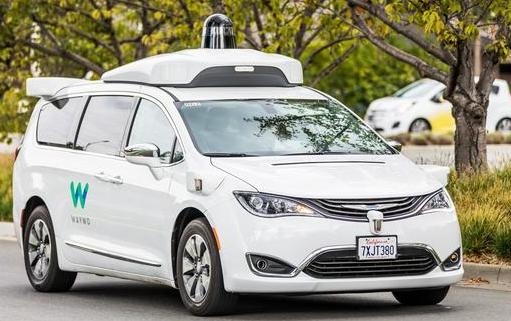
\includegraphics[width=.45\linewidth]{pictures/01/waymo}} \quad
  \subfloat[Tesla's Autopilot]
  {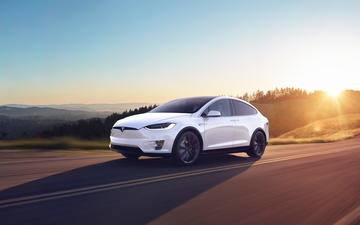
\includegraphics[width=.45\linewidth]{pictures/01/modelx}} \\
  \subfloat[Nutonomy's AV]
  {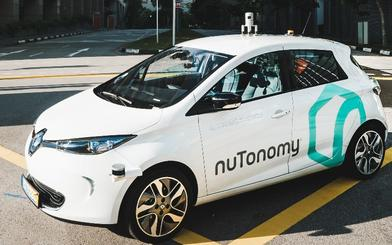
\includegraphics[width=.45\linewidth]{pictures/01/nutonomy}} \quad
  \subfloat[Optimus Ride's autobus]
  {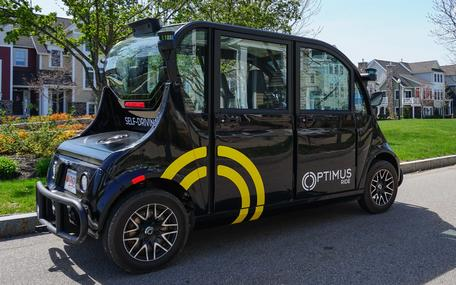
\includegraphics[width=.45\linewidth]{pictures/01/optimus}} 
  \caption[Current state of AVs]{Current state of AVs}
  \label{fig:auton_vehic}
\end{figure}

\subsection{Some history on Self-Driving Vehicles}

First attempts to build robotic vehicles date as early as 1920s \citeintro{Bimbraw2015} when the first radio controlled vehicles were designed. In the decade of 1980, there were serious attempts at building autonomous vehicles, such as the following projects:

\begin{itemize}

  \item \textbf{Prometheus} (Program for a European Traffic with Highest Efficiency and Unprecedented Safety) project: The aim of this project was to build a civilian car to navigate on highways or cities (\ie more structured environments) \citeintro{Xie1993, Flyte1995}. The vehicle chosen was a Mercedes-Benz van designed by Ernst Dickmanns and during test drives on highways it achieved a maximum speed of 96 km/h and drove for about 20 km\footnote{History on the car: \url{https://www.mbscottsdale.com/blog/mercedes-benz-whensday-the-prometheus-project/}}.

  \item \textbf{ALV} (Autonomous Land Vehicle) project: This project was developed by DARPA in America (Prometheus was from Europe) in collaboration with Carnegie Mellon University. The van employed was able to navigate, plan routes and avoid obstacles in coarser terrains than the Prometheus van for 5 km and at a speed of 20 km/h \citeintro{Leighty1986, Goto1987}. 
\end{itemize}

Both cars are shown in \autoref{fig:1980}.

\begin{figure}[htb]
  \centering
  \subfloat[Prometheus van]{
    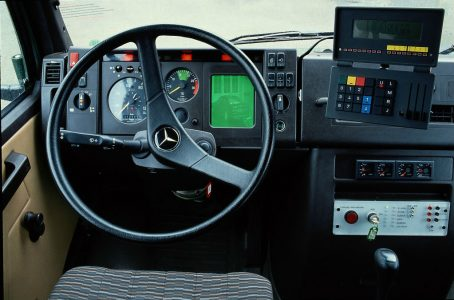
\includegraphics[width=.45\linewidth]{pictures/01/prometeus}
  } \quad
  \subfloat[DARPA's Autonomous Land Vehicle] {
  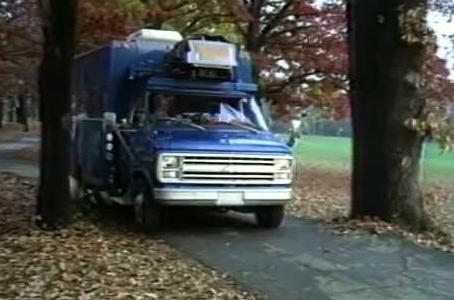
\includegraphics[width=.45\linewidth]{pictures/01/navlab}
  }
  \caption{The first serious attempts to build AVs}
  \label{fig:1980}
\end{figure}

In 2003, DARPA launched the Grand Challenge \footnote{\url{http://archive.darpa.mil/grandchallenge/}} to promote the development of unmanned vehicles. The Challenge was to drive a car autonomously through an unknown off-road terrain. More specifically, a 142 mile-long course across the Mojave desert in less than 10 hours \citeintro{Thrun2006} \citeintro{Seetharaman2006}. There were 107 teams registered, 15 of which made it to the race, although none of the participants drove further than 5\% of the total length. In 2005, the challenge was repeated and 5 teams managed to finish the race out of 197. Stanford University won that race with a car named Stanley (\autoref{fig:stanley}).

\begin{figure}[htb]
  \centering
  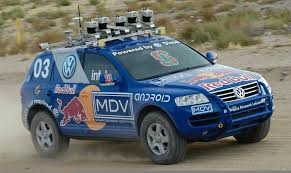
\includegraphics[width=.9\linewidth]{pictures/01/stanley2}
  \caption{DARPA Grand Challenge's first winner: STANLEY}
  \label{fig:stanley}
\end{figure} 

In 2009, Google launched the Self-Driving Car project that became a company named \href{https://waymo.com/}{Waymo}. Since its inception, this project has achieved very interesting milestones and it is the company that has driven more miles autonomously by far \citeintro{Hook2018}.

\subsection{Current state of autonomous driving and levels of autonomy}

Nowadays, virtually almost every car has some sort technology embedded in it, that provides it with a certain level of autonomy or 'intelligence'\citeintro{Litman2014}. Examples of these advancements are \citeintro{Thompson2017}:

\begin{itemize}

  \item \textbf{Self-parking}: A couple years ago, automakers like \href{https://www.toyota-europe.com/world-of-toyota/safety-technology/parking-aids}{Toyota}, \href{https://www.mbusa.com/mercedes/technology/videos/detail/class-SL_Class/title-convenience/videoId-bef758b451127410VgnVCM100000ccec1e35RCRD}{Mercedes} or \href{https://www.bmw.co.uk/bmw-ownership/connecteddrive/driver-assistance/intelligent-parking}{BMW} started developing cars that could find parking spots and maneuver the car to eventually fit it in. These technologies generally rely on ultrasonic sensors and cameras, taking into account cars' movement restrictions \citeintro{Paromtchik1996} (it will be explained in \autoref{ch:concepts}).

  \item \textbf{Automatic emergency-braking}: It detects imminent crashes and attempts to minimize the impact of them. These technology alerts the driver first with visual or sound warnings and if there is no response, the vehicle stops immediately.

  \item \textbf{Semi-autonomous drive system}: There are already cars on the market that can drive themselves autonomously on highway conditions. This is the case of \href{https://www.tesla.com/autopilot?redirect=no}{Tesla's Autopilot} or \href{https://media.gm.com/media/us/en/cadillac/news.detail.html/content/Pages/news/us/en/2017/apr/0410-supercruise.html}{Cadillac's Super Cruise}. These systems are capable of adapting to traffic conditions on highways and even steering on more complicated roads, but they still require the driver to pay attention to the road.

\end{itemize}

According to the Society of Automotive Engineers (SAE), there are 6 levels of automation\citeintro{SAE2015} as show on \autoref{fig:sae}.

\begin{figure}[htb]
  \myfloatalign
  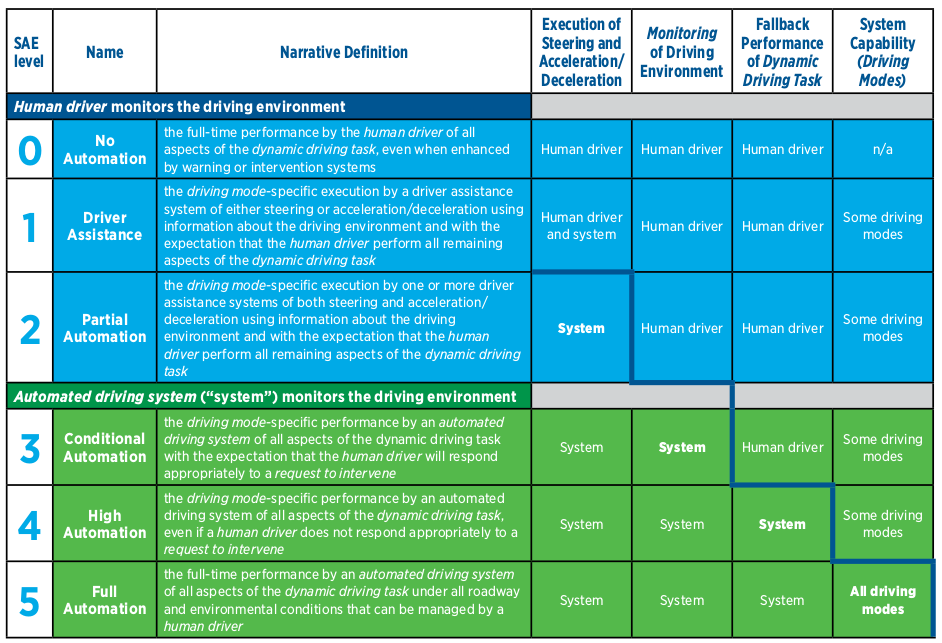
\includegraphics[width=\linewidth]{pictures/01/sae}
  \caption{Levels of Autonomy according to SAE}
  \label{fig:sae}
\end{figure} 

The first 3 levels (from 0 to 2) is where most cars lie nowadays, specially levels 1 and 2 thanks to the advances mentioned above. That means humans are still in charge of monitoring the environment. Tesla's Autopilot lies on level 3 though under certain conditions but it is still under development after the deadly crash in 2016 \citeintro{Hawkins2017}. With regards to level 4 autonomy (in other words, car is able to full self-drive but under certain road and weather conditions), Uber and Waymo announced plans to test driverless taxis last November \citeintro{Bergen2017, Lee2017}. 

Nevertheless, level 5 autonomous cars seem to be still a distant possibility. According to SAE (\autoref{fig:sae}), level 5 implies that no human intervention would be needed in any condition and that is not the case today, since AVs cannot be operated under heavy rain or snow conditions, unpaved roads or with diverse traffic \citeintro{Simonite2016}.

\subsection{Advantages of AVs}

The rise of self-driving cars and related technologies is not a product of coincidence rather than the general belief among scientists and industry that they will bring many benefits in terms of safety, productivity and wealth \citeintro{Litman2014}. In the following paragraphs, some of these advantages will be discussed.

\parunder{Road safety} According to the World Health Organization (WHO), every year around 1.25 million people lose their lives in car accidents and 20-50 million people get injured \citeintro{WHO2018}. In the United States human caused car accidents account for 90\% of the crashes \citeintro{Fagnant2015, UsDep2008}. By adopting AVs in large scales, distractions will happen less frequently, therefore reducing the number of deadly accidents.

\parunder{Improved mobility} The daily commute is one of the tasks AVs could help many drivers with. On average, it takes 26 minutes \citeintro{Uhlemann2016a} to go from home to work and back, time that could be spent doing more productive or rewarding tasks. Self-driving vehicles could be transformed into mobile bedrooms, playgrounds or offices to suit the demand of their users [citation], as it is Mercedes' self-driving concept car shows for example (\autoref{fig:mercedes})\footnote{https://www.youtube.com/watch?v=8aEWHdduPwc}.

\begin{figure}[htb]
  \myfloatalign
  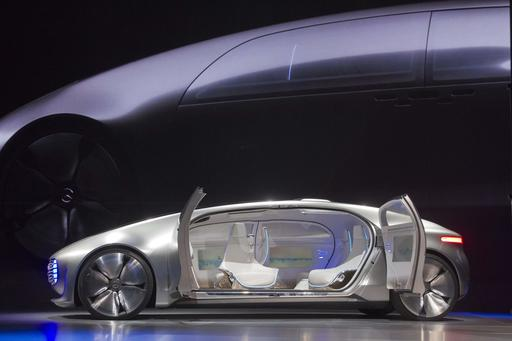
\includegraphics[width=\linewidth]{pictures/01/mercedes}
  \caption[Mercedes self-driving car]{Mercedes self-driving car}
  \label{fig:mercedes}
\end{figure} 

\parunder{Better Traffic Flow} Some researchers have shown that AVs can improve traffic flow \citeintro{Talebpour2016}. Since self-driving cars might be able to connect to other cars and features of the environment, and have lower response times, they can: 
\begin{enumerate} 
  \item Anticipate events faster and allow for smoother braking and acceleration.
  \item Use lanes and intersections more effectively by reducing gaps and platooning (\autoref{fig:platoon}).
\end{enumerate}

\begin{figure}[htb]
  \centering
  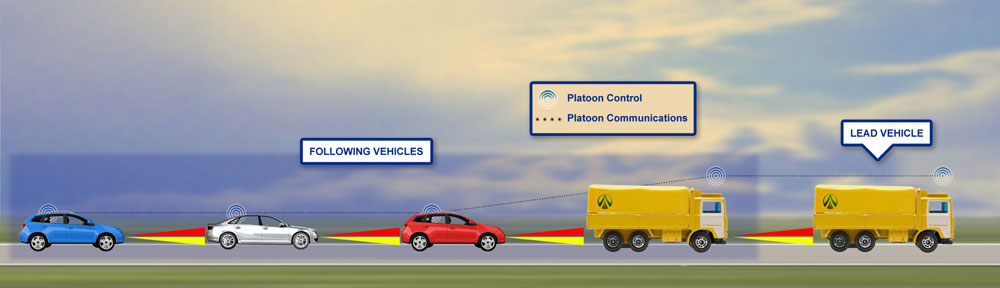
\includegraphics[width=\linewidth]{pictures/01/platoon}
  \caption{Platooning representation on a highway}
  \label{fig:platoon}
\end{figure}

\parunder{Shared Networks} One of the key attactives for AV technology is that it could enable new travelling modes (combining provate and public) such as communally-owned shared vehicles \citeintro{Haboucha2017}. Shared Autonomous Vehicles (SAVs) might potentially benefit the environment by reducing the need for car ownership and parking \citeintro{Fagnant2014a}. Users with similar destinations could share rides (in the same manner as with current carsharing services). However, the main advantage over what is available today, is that after the ride they could autonomously relocate themselves to more demanded areas, thus reducing the need for parking lots that could be transformed in green areas \citeintro{Litman2014}. 

\subsection{Disadvantages of AVs}

Even though self-driving technology has a vast potential to improve many aspects of society, it is not perfect and it raises concerns among researchers, policy makers and general public. Many of the positive aspects described above have their negative counterparts as it will be discussed in the next paragraphs.

\parunder{High costs} Even though costs could be reduced due to car reduction, the technology needed to transform a regular car into a self-driving one increases the prize dramatically. Each of the Light Detection and Ranging (LIDAR) sensors installed can cost between 30.000\$ and 85.000\$ \citeintro{Shchetko2014a} which makes AVs unaffordable for the vast majority of the population.  

\parunder{Liability and ethical questions} As AVs become more pervasive in everyday landscape, questions will arise when these vehicles are involved in any type of accident \citeintro{Fagnant2015}. When car's software fails, who is to blame: the software engineer, the company? How can an insurance company be convinced of the reliability of self-driving vehicles?

Moreover, if a crash is inevitable and the car has to decide between 2 evils, how can it make the decision? These ethical questions pose a major challenge when it comes to real world implementations and there is no clear answer. From MIT Media Lab's group \href{https://www.media.mit.edu/groups/scalable-cooperation/overview/}{Scalable Cooperation}, an initiative called Moral Machine \citeintro{Rahwan2016} was launched in order to create a discussion on these moral dilemmas and build a 'crowd-sourced' image of how intelligent machines should behave\footnote{A test can be taken with different scenarios: http://moralmachine.mit.edu/}.

\parunder{Public perception} Another issue to overcome is public perception. First of all, because when self-driving car technology reaches the mass market, professional drivers might start losing their jobs \citeintro{Litman2014}. Trust on the technology is an important obstacle to overcome, since few people will feel uncomfortable at first, being the technology new and not sufficiently tested \citeintro{Howard2014, Bansal2017}. 

\parunder{Safety and Security} Electronic security is a major concern for every major car- and policymaker, and for the general public \citeintro{Schoettle2014}. Hackers, terrorist groups or employees could target the intelligent system of the vehicles and cause major disruptions on the whole network \citeintro{Fagnant2015}, by forcing cars to collide or exposing users' locations.

\subsection{When will AVs hit the road?}

Due to these challenges and many other that arise when developing self-driving technologies, experts believe level 4 and 5 AVs will not be available to the general public until the 2040s--2050s \citeintro{Litman2014, Rowe2015}. 

\section{Shared mobility}

Shared mobility has already been mentioned as a future field of application of AVs, but the growth it has undergone in past years by itself is worth noting, since it has crutial implications for the future of transport in cities.

Many car sharing companies have already achieved a great market share like \href{https://www.zipcar.com/}{Zipcar}, \href{https://www.car2go.com/ES/en/}{Car2Go}, or even \href{https://www.uber.com/en-ES/ride/uberpool/}{Uber}'s latest services. However, this section will focus on bicycle sharing systems, due to their applications and benefits for cities across the world.

\subsection{What is bicycle sharing?}

Bicycle sharing or bikesharing corresponds to the public shared use of bicycle fleets that has gained attention these past years \citeintro{DeMaio2009, Shaheen2010} in many regions of the world such as Europe, US and China.

The case of China is specially striking, since many bikesharing startups have sprung out in the past years, and the biggest companies among those, \href{https://www.ofo.com/es/en}{Ofo} and \href{https://mobike.com/global/}{Mobike}, already have 19 million bikes across the world \citeintro{Yang2018}.

Nevertheless, bicycle sharing it is not a radically new concept from this century. In fact, its origins trace back to the 1960s and there have 3 generations in bikesharing history \citeintro{DeMaio2009}:

\begin{itemize}

  \item The first generation started in 1965 and the concept was to provide with ordinary bikes that could be parked anywhere. However, bikes were vandalized very often.

  \item Second generation was born in 1993, when bikes had to be parked on specific docks or stations. Although it improved the previous versions, bicycles were still subject to theft due to user anonimity.

  \item Third generation (the current one) bikes already incoporate smart technologies like electronic locks or bicycle tracking to improve security.

\end{itemize}

The rise of this transportation method is not casual since it comes as an answer to 3 key aspects in cities \citeintro{DeMaio2009}:

\begin{itemize}

  \item \textbf{Increased cycle usage}: This way healthier lifestyles are promoted in urban environments.

  \item \textbf{Increase first/last mile connection}: Bike sharing can provide its users with connection from their homes/working areas to other means of transport such as buses, trains or subway. Moreover, bike fleets can be used to tranport not only people but packages and other goods across the city, thus avoiding traffic congestions caused by larger vans or trucks.

  \item \textbf{Reduce environmental impacts}: Biking is an emission--free means of transport and therefore it can help mitigate common concerns in cities like global climate change, energy supply or varying fuel prices \citeintro{Shaheen2010}.

\end{itemize} 

\subsection{What are the current disadvantages of these approaches?}

Again there is no perfect solution to urban transportation and bicycle sharing suffers essentially from 2 issues.

\paragraph{System rebalancing:} The first one, and this occurs to shared automobiles as well, is that they have to be manually relocated in order to guarantee the balance of the system. This implies arranging a logistics network around the city in order to ensure every area they are operated within has a minimum amount of bikes.
  
\paragraph{bike Cemeteries:} Because of these attempts to equilibrate the network, companies must provide with a higher amount of bicycles than necessary and keep higher stocks, all resulting in greater maintenance costs and many times bicycles end up in in landfills. Combining this with market saturation as it is happening in China's markets, 'bike cemeteries' are being formed in the outskirts of cities like Shanghai or Beijing (\autoref{fig:cemetery}) \citeintro{Campbell2018}.

\begin{figure}[htb]
  \centering
  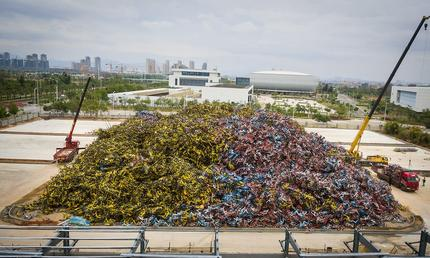
\includegraphics[width=.9\linewidth]{pictures/01/cemetery3}
  \caption[Bike cemeteries outside cities]{Unused bicycles end up forming immense cementeries around cities}
  \label{fig:cemetery}
\end{figure}  

\section{Persuasive Electric Vehicle (PEV)}

\subsection{MIT Media Lab: Home of Innovation}

To understand the PEV project, it is necessary first to put some context on the place of its inception, the Media Lab. According to their website, Media Lab is "an antidisciplinary research lab working to invent the future"\footnote{https://www.media.mit.edu/research/?filter=groups}. In fact it is a place that gathers all sorts of people from various backgrounds such as Arts, Sociology, Computer Science or Engineering and aims at developing ideas that bring technology closer to humans. Since its foundation in 1985, more than 150 companies have spun out of its doors\footnote{https://www.media.mit.edu/about/spin-off-companies/}.

Some of the notable projects are:

\begin{itemize}
  \item \textbf{Scratch programming language}: It is a block-based language initially developed for children but that it is used by people all ages around the world \citeintro{Resnick2009}

  \item \textbf{Harmonix}: Game development company that launched \href{http://www.harmonixmusic.com/}{Rock Band and Guitar Hero}.

  \item \textbf{E-ink}: Company that developed the electronic ink, now used in e-readers around the world \citeintro{Jacobson2003}.
\end{itemize}

\subsection{City Science and its mission}

\href{https://www.media.mit.edu/groups/city-science/overview/}{City Science} is one of the 25 groups of this ecosystem and it is where the PEV is located. The group, led by Professor Kent Larson, is aware of the challeges cities will face in the coming years and is focused on developing platforms and tools that will improve life in cities \citeintro{Larson2012}. There are 3 main research topics at City Science:

\begin{itemize}

  \item \textbf{CityScope}: It is a platform that aims at providing tools for cities and urban planners to model and design infrastructures with the use of simulations and real time data \citeintro{Grignard2018}. The whole system is built around a Lego table, where decision makers can 'play' and see the effects of their solutions in real-time (\autoref{fig:cityscience}).

  \item \textbf{Changing Places}: This group focuses on developing responsive places to live and work in future cities. 2 of the most famous projects are Cityhome which later became the spinoff \href{https://www.orisystems.com/}{Ori} which provides robotic furniture (\autoref{fig:cityscience}), and Escape Pod, a transformable space for either working or resting.

  \item \textbf{Mobility-on-Demand}: This group is focused on efficient shared--use mobility systems and its main project is the aforementioned \textbf{PEV} which will be explained in more detail in the following lines.

\end{itemize}

\begin{figure}[ht]
  \centering
  \subfloat[CityScope]{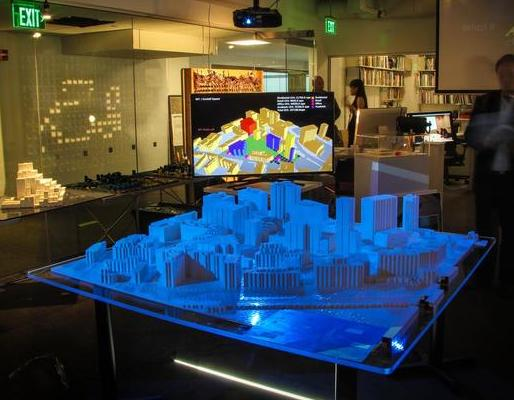
\includegraphics[width=.45\linewidth]{pictures/01/cityscope}} \quad
  \subfloat[Ori system]{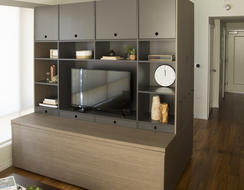
\includegraphics[width=.45\linewidth]{pictures/01/ori}}
  \caption{City Science's CityScope and Ori platforms}
  \label{fig:cityscience}
\end{figure} 

\subsection{Reason for the PEV}

The \href{https://www.media.mit.edu/projects/pev/overview/}{PEV} is an autonomous, lightweight, low--cost, electric and shared tricycle (\autoref{fig:pev}) that aims to be an alternative to both autonomous vehicles and bikesharing systems.

\begin{figure}[htb]
  \centering
  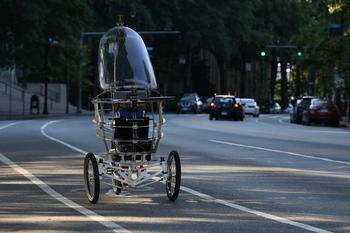
\includegraphics[width=\linewidth]{pictures/01/pev}
  \caption[PEV on the streets]{PEV on the steets of Cambridge, Massachusetts (August 2017)}
  \label{fig:pev}
\end{figure}

The PEV would be operated in 2 different modes:

\begin{itemize}

  \item \textbf{People mover}: People would be able to call a PEV with a phone app (like Uber) and the vehicle would come to the user autonomously. Then the requester would have to ride it to the destination and after the ride, the PEV would leave on its own to another location.

  \item \textbf{Package delivery}: PEV could be used as a package delivery system while user demand is low (for example, at working hours). This way it could help reduce traffic congestion caused in cities by trucks or vans.

\end{itemize}  

It has already been explained taht both AVs and bikesharing systems have their downsides. The idea of the PEV was born to tackle the issues that arise on these approaches as \autoref{tab:avpev} shows.

\begin{table}[htb]
  \centering
  \resizebox{\textwidth}{!}{\begin{tabular}{p{3cm}p{4.5cm}p{4cm}p{4.5cm}}
  \hline
  \multicolumn{1}{c}{\textbf{Aspect}} & \multicolumn{1}{c}{\textbf{AVs}} & \multicolumn{1}{c}{\textbf{Bike Sharing}} & \multicolumn{1}{c}{\textbf{PEV}} \\ \hline
  \textbf{Environmental Impact} & Even though they might reduce traffic, environmental cost will be high & Minimal impact & Slightly bigger (when in autonomous mode) but minimal when riding it \\ \hline
  \textbf{Healthy lifestyle} & They do not promote healthier lifestyles & Cycle usage increases physical activity & Passengers will have to pedal, thus promoting a healthier transport \\ \hline
  \textbf{Infrastructure} & AVs need high-quality roads and special infrastructure that might be costly & They can run on current bike-lanes & It is designed to fit on bike lanes, so it would require less infrastructural support \\ \hline
  \textbf{Road safety} & They are subject to strict regulations due to their risk, so that might slow down their deployment & It is less dangerous so regulation is not as strict & As it it is lightweigth and will operate at low speeds on bike lanes, risk will be lower than with self-driving cars. Therefore deplyoment might be faster \\ \hline
  \textbf{Parking} & They need minimal parking & They need a notable amount of stations & They need minimal parking \\ \hline
  \textbf{Relocation} & They can relocate automatically based on demand & The need to be manually relocated & They can relocate automatically based on demand \\ \hline                                                                                                    
  \end{tabular}}
  \caption[AVs, bikesharing systems and PEV]{Comparison between AVs, bikesharing systems and PEV}
  \label{tab:avpev}
  \end{table}

\section{Thesis Structure}

This thesis is divided as follows:

\begin{itemize}
  \item \textbf{Chapter 2} explores the current technologies available for autonomous vehicles and describes the fundamental elements of the main aspects of self-driving vehicles.

  \item \textbf{Chapter 3} describes the field of Simultaneous Localization and Mapping (SLAM) more thoroughly, as well as providing with the latest approaches.
  
  \item \textbf{Chapter 4} analyzes different slam algorithms applied on a small autonomous robotic platform, that served as a testbed for the PEV.

  \item \textbf{Chapter 5} analyzes the slam approach on the PEV, and what are the best configurations for different scenarios.

  \item \textbf{Chapter 6} shows a simple budget for the project and its timeline.

  \item \textbf{Chapter 7} provides with conclusions on the results obtained on both platforms, improvements that could be tackled and sets the next steps for these vehicles.

\end{itemize} 

 % Chapter 1
\cleardoublepage % Empty page before the start of the next part

% Techniques, sensors and frameworks used in autonomous technologies

\chapter{Autonomous Vehicle concepts}
\label{ch:concepts}

In essence, AVs are robots (with 2 degrees of freedom, generally) and more specifically fall in the branch called \textbf{Mobile Robotics}. The following pages will explore the basic concepts of it and what are the tools available to tackle this field.

\section{What is Mobile Robotics}

\subsection{Examples of mobile robotics}

The use of robots to assist or substitute human labour dates back to the 1960s \citeauton{Craig2004} with industrial manipulators and to this day remains as one of the most successful applications of this field. However, generally these robots lack moving capabilities, thus they are limited to a narrow operating environment. 

Mobile Robotics is a relatively recent branch of robotics which aims at developing platforms with moving capabilities \citeauton{Siegwart2004}, in order to achieve tasks that are impossible to do for fixed robots.

Applications in the field of mobile robotics range from:

\begin{itemize}
  \item \textbf{Material delivery}: This is the case for Kiva Systems, company acquired by Amazon in 2012, and whose core idea is to use swarms of mini-robots to transport materials across the warehouse \citeauton{Andrea2012}. Mobile robots (in this case drones) have started to be used by companies like Amazon, Google and DHL to develop last mile delivery logistics \citeauton{Menouar2017a}.

  \item \textbf{Home applications}: This field is where the house cleaning robots called Roomba developed by \href{https://www.irobot.es/}{iRobot} lie. These platforms are equipped with different sensors that allow them to map their environment and navigate in order to clean the rooms of the household \citeauton{Woyke2017}.

  \begin{figure}[t]
    \centering
    \subfloat[Kiva system's robot in a warehouse]{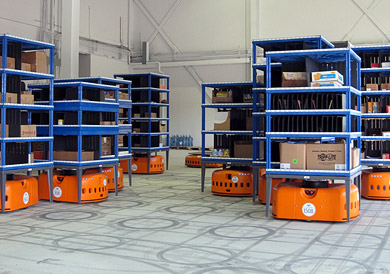
\includegraphics[width=.45\linewidth]{pictures/02/kiva}} \quad
    \subfloat[iRobot's Roomba]{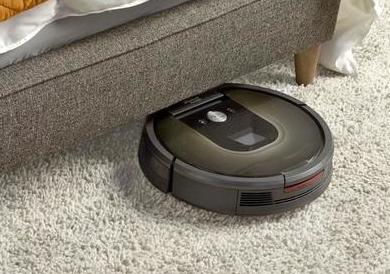
\includegraphics[width=0.45\linewidth]{pictures/02/roomba}}   
    \label{fig:kivarromba}
    \caption[Kiva Systems and Roomba]{Kiva System's robots and Roomba share some design principles}
  \end{figure} 

  \item \textbf{Autonomous Vehicles}: As it was shon on \autoref{ch:intro}, there are many possible areas where self-driving vehicles could be applied.

  \item \textbf{Unknown Environment Exploration}: Robots with moving capabilities are employed to explore unknown environments in rescue missions \citeauton{Bernard2011} or in other planets \citeauton{Grotzinger2013}.
  
  \item \textbf{Defense}: As it has happened with many other scientific advances in history, there is interest in developing mobile robotics with military goals. This is the case of Boston based company \href{https://www.bostondynamics.com/}{Boston Dynamics} and their four-legged robot BigDog \citeauton{Raibert2008} capable of travelling through diverse outdoor terrains.

  \begin{figure}[t]
    \centering
    \subfloat[NASA's Curiosity rover on Mars]{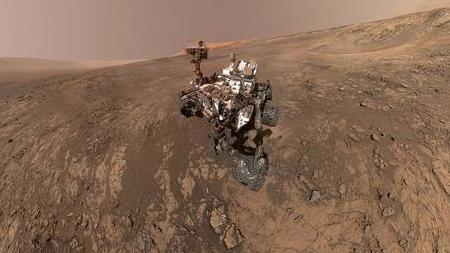
\includegraphics[width=.45\linewidth]{pictures/02/curiosity}} \quad
    \subfloat[Boston Dynamic's SpotMini (2018)]{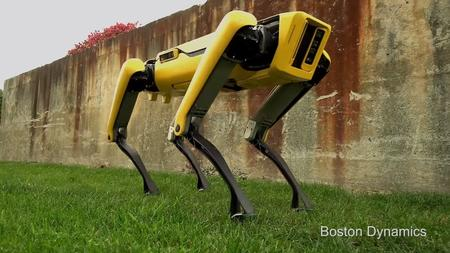
\includegraphics[width=0.45\linewidth]{pictures/02/boston}}   
    \label{fig:curiosityboston}
    \caption[Curiosity and SpotMini robots]{Built to explore the unknown, with different goals in mind}
  \end{figure}
\end{itemize}

\subsection{Robot control paradigms}

The paradigms of control for mobile robotics are very similar to the ones used in robotics and control in general \citeauton{Burgard2017}. Many of the robots mentioned above follow the classical paradigm of sense-plan-act (\autoref{fig:classiccontrol}). The explanation of it is very straightforward: robot senses the environment, then feeds its algorithms with that data and produces an output, that goes into the system's actuators. That response is measured in the next iteration, forming a closed-loop.

\begin{figure}[htb]
  \centering
  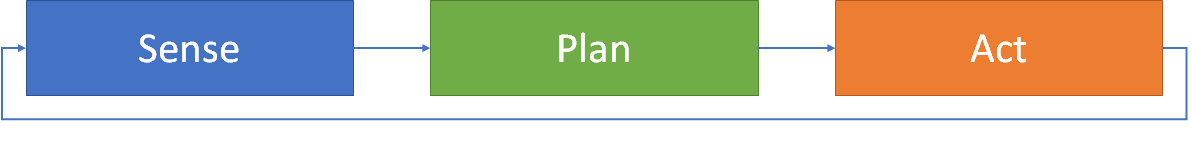
\includegraphics[width=\linewidth]{pictures/02/controlclassic}
  \caption{Classical control paradigm}
  \label{fig:classiccontrol}
\end{figure}

However, this approach requires a larger amount for computing power, which is not suitable for smaller platforms like the Roomba or other home robotics \citeauton{Burgard2017}. Therefore, these types of robots used a more reactive paradigm, where the planning step is removed and substituted by direct mapping of the sensor inputs to specific commands (\autoref{fig:reactive}).

\begin{figure}[htb]
  \centering
  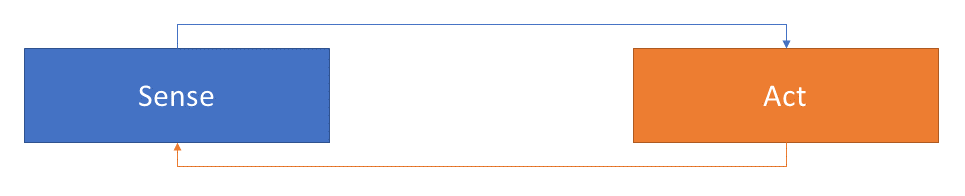
\includegraphics[width=.9\linewidth]{pictures/02/reactive}
  \caption{Reactive control paradigm}
  \label{fig:reactive}
\end{figure}

For the case of self-driving vehicles, the first approach is more suitable, since situations these robots encounter tend to be more complex and require a greater understanding of the environment \citeauton{Siegwart2004}. That is why the classical paradigm is preferred and used in AVs. \autoref{fig:control}, shows a more fine grained description of the control of an autonomous vehicle like the PEV.

\begin{figure}[htb]
  \centering
  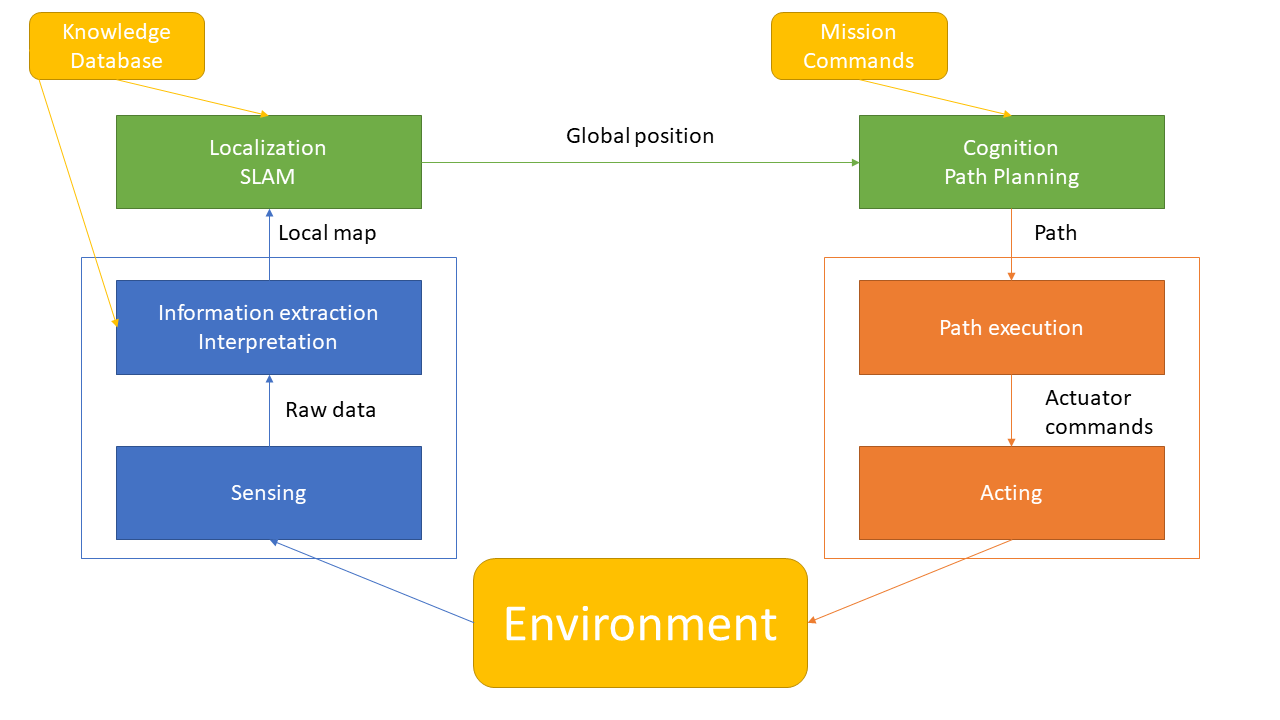
\includegraphics[width=\linewidth]{pictures/02/control}
  \caption{Extended control paradigm for mobile robots}
  \label{fig:control}
\end{figure}

The 3 aspects of control are present (sense-plan-act) but each one is subdivided in different categories. Each one of these constitutes is equally important to consider when building an autonomous platform and they will be described in the following section.

\section{Fundamentals of mobile robotics}

\subsection{Control and Locomotion}

It has been mentioned before that classical robotic arms operate generally fixed to the ground in environments with moving objects, whereas mobile ones are in charge of navigating in mostly static scenarios. Therefore, it can be deduced that mobile robot's most fundamental feature is \textbf{locomotion} \citeauton{Siegwart2004} and it plays an important role on the design of the platform. 

Locomotion can take various forms but the most studied mobile robots are \textbf{legged} and \textbf{wheeled} (\autoref{fig:legwheel}). 

\begin{figure}[htb]
  \centering
  \subfloat[Boston Dynamics' Atlas]{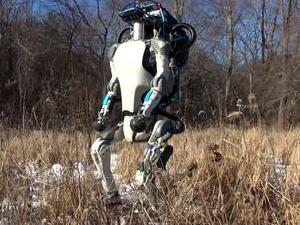
\includegraphics[width=.45\linewidth]{pictures/02/atlas}} \quad
  \subfloat[Yujin Robot's turtlebot]{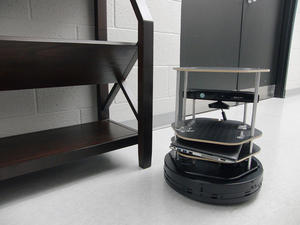
\includegraphics[width=.45\linewidth]{pictures/02/turtlebot}}
  \caption{Legged vs Wheeled robots}
  \label{fig:legwheel}
\end{figure}  

This thesis explores more in detail wheeled locomotion, since it is the basis for both robots that will be described in \autoref{ch:nexus} and \autoref{ch:pev}.

The wheel is by far the most popular mechanism for movement and there are various types \citeauton{Burgard2017a}:

\begin{itemize}
  \item \textbf{Differential drive}: These robots have 2 driving wheels and having each a motor attached. Movement varies due to 'differences' in the speed of both wheels.

  \item \textbf{Car drive (Ackerman steering)}: In this case one motor is in charge of the forward movement, whereas the other one steers the wheels.

  \item \textbf{Omnidirectional drive}: These robots are capable of moving in any direction at any time by using spherical, castor or Swedish wheels (\autoref{fig:omni}).

  \item \textbf{Tracked locomotion}: When driving through loose terrains, wheels are put on a track so that the vehicle gains stability and maneuverability (for example in tanks as shown in \autoref{fig:tank}).

\end{itemize}

\begin{figure}[htb]
  \centering
  \subfloat[Robot with Omnidirectional drive \label{fig:omni}]{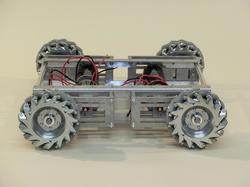
\includegraphics[width=.45\linewidth]{pictures/02/omni}} \quad
  \subfloat[Tanks make use of tracked locomotion \label{fig:tank}]{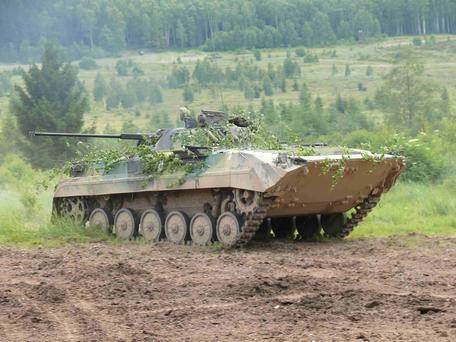
\includegraphics[width=.45\linewidth]{pictures/02/tank}}
  \caption{Omnidirectional and tracked motion examples}
  \label{fig:omnitank}
\end{figure}  

In the next paragraphs, differential drive and ackermann steering will be described in more detail, since those models were used in the Nexus Robot and the PEV respectively.

\parunder{Differential drive} There are many configurations for differential drive robots as it is illustrated in \autoref{fig:diff}. Lets suppose that right and left wheels rotate at velocities $v_r$ and $v_l$ respectively, and that they are separated a distance $L$ (\autoref{fig:diffeq}).

\begin{figure}[htb]
  \centering
  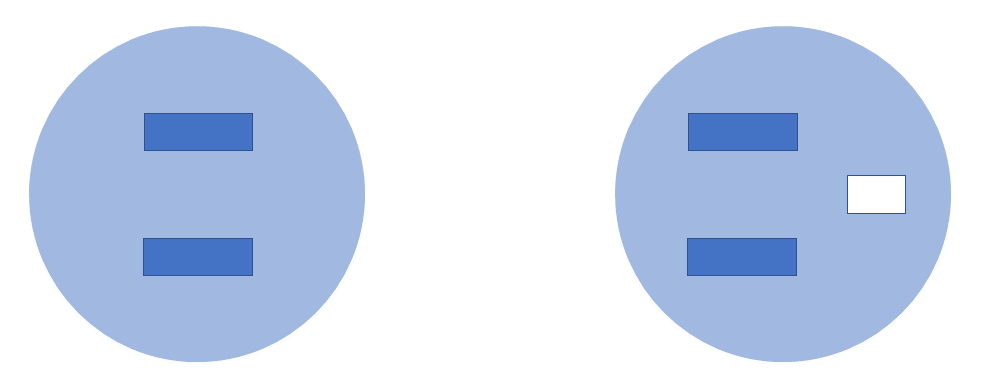
\includegraphics[width=.7\linewidth]{pictures/02/diff}
  \caption[Differential drive modes]{Differential drive modes: 2 motorized wheels (left) or 2 motorized wheels + caster (right)}
  \label{fig:diff}
\end{figure}

\begin{figure}[htb]
  \centering
  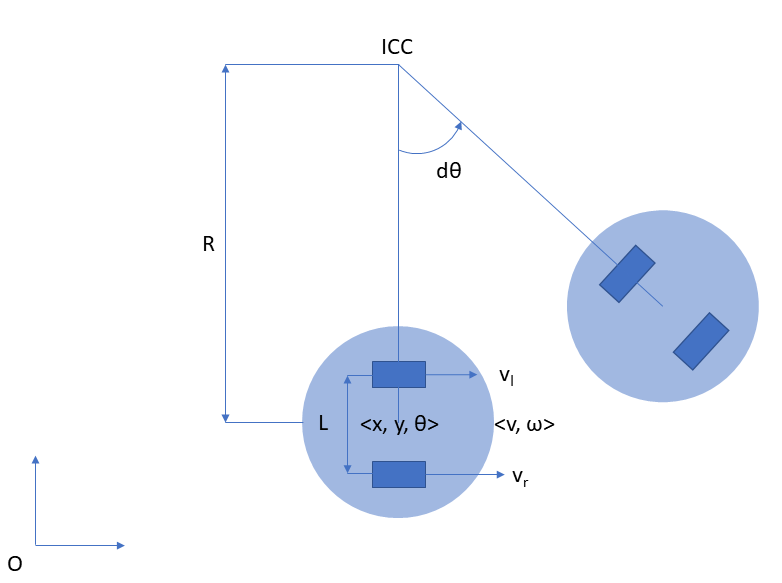
\includegraphics[width=.9\linewidth]{pictures/02/diffeq}
  \caption{Instantaneous movement of a differential drive robot}
  \label{fig:diffeq}
\end{figure}

The movement of the robot is modelled as a rotation at angular speed $\omega$ around the Instantaneous Center of Curvature, ICC (it is shown as $R$ in \autoref{fig:diffeq}).

Both wheel velocities, R and $\omega$ are related through the following equations:
\begin{gather}
  v_l = \omega\cdot(R-\frac{L}{2})\\
  v_r = \omega\cdot(R+\frac{L}{2})
  \label{eq:vrl}
\end{gather} 

From which both $R$ and $\omega$ can be obtained:
\begin{gather}
  R = \frac{L}{2}\cdot\frac{v_r + v_l}{v_r - v_l}\\
  \omega = \frac{v_r - v_l}{L}
  \label{eq:Rw}
\end{gather}  

From these values, the velocity of the robot, $v$ is deduced:
\begin{equation}
  v = \omega \cdot R = \frac{v_r + v_l}{2} 
  \label{eq:v}
\end{equation}

From these equations it can be deduced that differential drive vehicles are able to perform either pure translations (if $v_r$ and $v_l$ are equal) rotate in place (if $v_r$ and $v_l$ are opposite) \citeauton{LaValle2006}.

Both linear and angular velocities are expressed in the local frames, so they are transformed to the base frame:
\begin{gather}
  ^{0}\mathbf{v} = ^{0}\!\!\mathbf{R}_A\cdot^{A}\!\mathbf{v} \label{eq:traf} \\
\begin{bmatrix} \dot{x} \\ \dot{y} \\ \dot{\theta} \end{bmatrix} = 
  \begin{pmatrix} cos\,\theta & -sin\,\theta & 0 \\ sin\,\theta & cos\,\theta & 0 \\ 0 & 0 & 1 \end{pmatrix} \cdot \begin{bmatrix} v \\ 0 \\ \omega \end{bmatrix} = 
  \begin{bmatrix} v\cdot cos\,\theta \\ v\cdot sin\,\theta \\ \omega \end{bmatrix}
    \label{eq:vwtraf}
\end{gather}  

The trajectory is computed by integrating each term over time:
\begin{equation}
  \begin{bmatrix} x \\ y \\ \theta \end{bmatrix} = 
    \begin{bmatrix} \int\limits_0^t v(t) cos(t) dt\\ \int\limits_0^t v(t) sin(t) dt \\ \int\limits_0^t\omega(t)dt \end{bmatrix} = 
    \begin{bmatrix} \frac{1}{2}\!\int\limits_0^t (v_r(t)+v_l(t)) cos(t) dt\\ \frac{1}{2}\!\int\limits_0^t (v_r(t)+v_l(t)) sin(t) dt \\ \frac{1}{L}\!\int\limits_0^t(v_r(t) - v_l(t))dt \end{bmatrix}
\end{equation}  

\parunder{Ackerman steering}

There are various modifications of the Ackerman steering vehicle as well (\autoref{fig:ack}). These vehicles need 2 commands, the drive speed $v$ and the steering angle $\varphi$. Supposing a robot with Ackerman steering whose wheel distance is L, and that the movement can be modelled as a rotation around the ICC (same as differential drive).

\begin{figure}[htb]
  \centering
  
\includegraphics[width=\linewidth]{pictures/02/ack}
  \caption[Ackermann drive modes]{Ackerman drive modes: bicycle (left), tricycle (center), car (right)}
  \label{fig:ack}
\end{figure}

Obtaining the linear speed is trvial (it is s itself), thus only the calculation of the angular speed is needed. Looking at \autoref{fig:ackeq}, it can be seen that:
\begin{gather}
  v = \rho\cdot\omega \\
  \frac{L}{\rho} = tan\,\varphi
\end{gather}  

This yields the result for $\omega$:
\begin{equation}
  \omega = \frac{v}{L}tan\,\varphi
\end{equation} 

The velocities in global coordinates and the translation are computed with the same equations the differential drive robots use. However, there is a fundamental difference between both locomotions: for Ackerman steering robots, it is not possible to rotate in place since that would require the backwheels to slide instead of roll \citeauton{LaValle2006}.

\begin{figure}[htb]
  \centering
  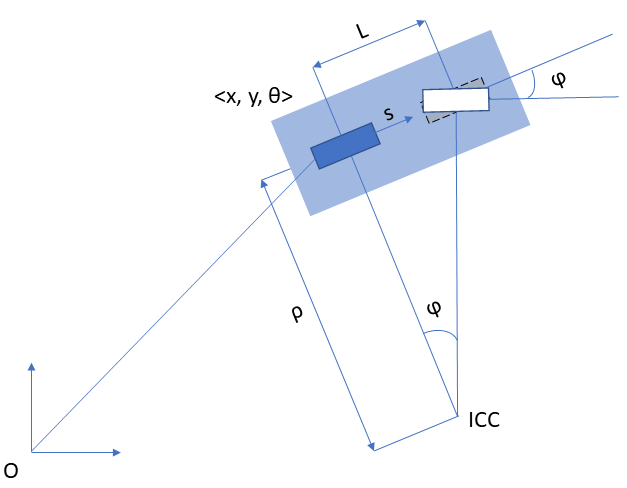
\includegraphics[width=.9\linewidth]{pictures/02/ackeq}
  \caption{Instantaneous movement of an Ackerman drive robot}
  \label{fig:ackeq}
\end{figure}

\subsection{Perception} \label{sub:perception}

Apart from kinematics, acquiring information from the environment is an essential feature, not only of mobile robotics but many other systems \citeauton{Siegwart2004}. \textbf{Sensors} are the ones in charge of that information gathering and they can be divided in \citeauton{Burgard2017b, Burgard2017c}:
\begin{itemize}
  \item \textbf{Active/Passive}: Active sensors emit energy to the environment and measure the response (lasers, radars) and passive sensors measure external inputs (cameras, tactiles).

  \item \textbf{Proprioceptive/Exteroceptive}: Whether the sensor measures internal (speed, joint angles) or external (distance, sound) values.
\end{itemize} 

Sensors can be categorized based on their specific function as well. In the next paragraphs some of these sensors will be described, specially the ones used on the PEV, but there is a wealth of other options that are more suited to other applications \citeauton{Fossen2017, Borenstein1996}.

\parunder{Dead--reckoning and Odometry sensors} Dead--reckoning is the process of determining the current position based on previous state knowledge and the undertaken actions \citeauton{Borenstein1996, Borenstein1997}. One of the most important and widely used implementations of dead--reckoning is \textbf{odometry}, since it is accurate in the short--term, although it drifts over time \citeauton{Borenstein1997}. 

The most used sensors to measure odometry are \textbf{optical encoders}, which consists of a light source passing through a punched disc producing a number of pulses per rotation. Counting the number of pulses (p) in a $\Delta t$, given that the disc has N pulses per revolution can provide the angular velocity:
\begin{equation}
  \omega = \frac{p}{N}\frac{2\pi}{\Delta t}\,\left[\frac{rad}{s}\right]
  \label{eq:odometer}
\end{equation}

If a second channel is added and shifted 90 degrees, rotation direction can be measured as well as position determination becomes more precise (\autoref{fig:encoder}).

\begin{figure}[htb]
  \centering
  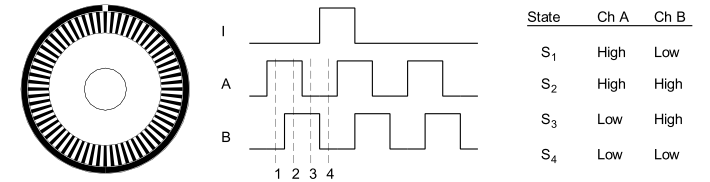
\includegraphics[width=\linewidth]{pictures/02/encoder}
  \caption{Rotary encoder working principle}
  \label{fig:encoder}
\end{figure}  

\parunder{Heading sensors} Heading sensors can help compensate the errors produced in odometry by small differences in orientation \citeauton{Borenstein1996}. This type of sensors are also called \textbf{Inertial sensors} and there are mainly 2 types \citeauton{Borenstein1997}:

\begin{itemize}
  \item \textbf{Accelerometers}: They measure acceleration in one or more axes. However, they perform poorly on many mobile robot applications if used alone.

  \item \textbf{Gyroscopes}: These sensors can measure orientation on 3 axes and are of a notable importance since they correct the odometry measurements when there are small orientation changes.
\end{itemize}  

Recently, another type of sensor has arisen in the field of mobile robotics called \textbf{Inertial Measurment Unit (IMU)}, which combines both accelerometer and gyroscope (sometimes adding a magnetometer for heading).

\parunder{Active/Passive beacons} The principle behind this technology has been used for centuries and it is to determine the absolute position of the robot based on the distance to landmarks or objects whose location is well known \citeauton{Siegwart2004}. This mapping of the position of the robot is done via \textbf{trilateration} or \textbf{triangulation} \citeauton{Borenstein1997}.

Here 2 different systems can be defined: \textbf{Ground--based beacons} and \textbf{Global Positioning System (GPS)}. They vary in that the former uses features or infrastructures located on the ground whereas the latter makes use of a network of satellites specifically built for that purpose (\autoref{fig:gpssch}). 

\begin{figure}[htb]
  \centering
  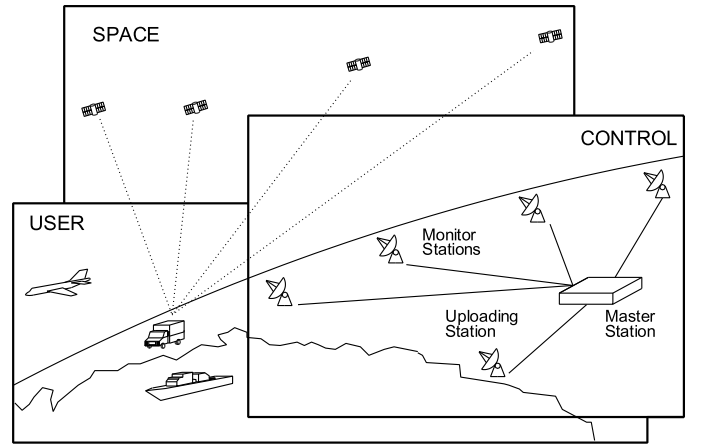
\includegraphics[width=\linewidth]{pictures/02/gps}
  \caption{GPS network overview}
  \label{fig:gpssch}
\end{figure} 

One of the issues these technologie has is that even though it works satisfactorily in outdoor 'open' environments, it is not as suitable in indoor or more 'closed' regions (urban areas with large buildings) \citeauton{Borenstein1996, Borenstein1997}. 

\parunder{Active ranging sensors} This sensors are mostly used for map building and localization. Among all the varieties, the \textbf{Time--of--flight} sensors are the most utilized. These devices send a wave (sound or electromagnetic) and knowing the speed at which they operate, the distance travelled is calculated:
\begin{equation}
  d = \frac{v\cdot t}{2}
  \label{eq:tof}
\end{equation} 

2 types of time-of-flight sensors will be described:
\begin{itemize}
  \item \textbf{Ultrasonic}: This kind of sensor sends a packet pressure waves to determine distance of objects. However, their range goes from 12 cm to 5 m making them unfit for large environments.

  \item \textbf{Laser rangefinders or LIDARs}: It improves the ultrasonic sensor by using infrared light, and it normally adds a rotating mirror so it can cover a wider area. The range of these sensors goes up to 300 m\footnote{https://velodynelidar.com/vls-128.html}. Generally, LiDAR output is a detailed 2D or 3D pointcloud of the surroundings, which often is better than camera+radar based systems. That is why is considered to be the single most important sensor in Autonomous Vehicles \citeauton{Davies2018} and it is also one of the most expensive components.
\end{itemize}  

\parunder{Vision--based sensors} Vision is one of the most powerful senses humans have. It provides with a great deal of information about the surrounding environments and currently there is a lot of effort into building machines with similar capabilities. Recent advances in machine--learning (and deep--learning in particular) \citeauton{LeCun2015}, combined with the existence of many frameworks such as \href{https://www.tensorflow.org/}{Tensorflow} have improved tasks that previously where extremely difficult, such as object detection, scene understanding or lane detection.

The most used vision--based sensors are cameras, among which 2 types can be diferenced:

\begin{itemize}
  \item \textbf{Monocular cameras}: These are well known devices, that have been available in the market for decades.

  \item \textbf{Stereo cameras}: Essentially, the concept is to combine the input images of 2 cameras that watch the scene from different perspectives, and by comparing points that appear on both (conjugate pair), depth information can be obtained (\autoref{fig:zed}).
  \begin{figure}[htb]
    \centering
    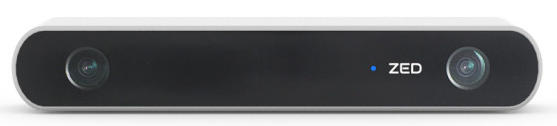
\includegraphics[width=.8\linewidth]{pictures/02/zed}
    \caption{\href{https://www.stereolabs.com/}{ZED} stereo camera}
    \label{fig:zed}
  \end{figure} 
\end{itemize}  

\subsection{Localization} \label{sub:localization}

The problem of localization (which is related to the problem of SLAM that will be discussed in \autoref{ch:slam}) is to determine the position of the robot within the environment \citeauton{Siegwart2004, Thrun2005}.

Recalling the control paradigms in Figures \ref{fig:control} and \ref{fig:reactive}, it is not difficult to see that the former needs a map--based localization system whilst the latter does not. However, the reactive paradigm is not robust to changes in the environment, since it would require to change the rules every time it changed. The classic control one is more scalable beause just by giving the robot another map, it could start navigating in a shorter amount of time.

When a robot is localized it means that the pose of the robot $\mathbf{x_t} = (x\,\, y\,\, \theta)$ is known with respect to the global frame. Nevertheless, pose cannot be sensed, it must be inferred from other sources and sensors are not noise--free, thus making the problem of localization a difficult one \citeauton{Thrun2005}.

\newpage
\parunder{Map representation} The quality of the map is a critical component for a robust localization, therefore much attention has to be paid when choosing a representation \citeauton{Siegwart2004}.

There are mainly 2 manners of representing maps:
\begin{itemize}
  \item \textbf{Continuous representation}: They contain the exact description of their environment. The main advantage is their accuracy at a higher computational cost.
  
  \item \textbf{Decomposed representation}: These type of maps are a higher level abstraction of the area, which results in loss of accuracy but may be useful if the jey features are preserved. One of the most common forms are \textbf{occupancy grid maps}, where the map is discretized an assigned a value if occupied or free.
\end{itemize}  

\parunder{Dimensions of localization} Localization algorithms have a number of divisions \citeauton{Thrun2005}:
\begin{itemize}
  \item \textbf{Global/Local}: In global localization the initial position is unknown, whereas in the local one it is known to be confined in a certain region.

  \item \textbf{Static/Dynamic}: The former are those whose objects remain still and the latter have features that change their position over time.

  \item \textbf{Passive/Active}: In passive localization, the algorithm is limited to observation. In active localization, the algorithm can affect the robot motion to facilitate it.
\end{itemize}  

\parunder{Localization approaches} With regards to the specific algorithms for localization, the main approach is \textbf{probabilistic localization} \citeauton{Thrun2005}. In these branch are included Markov, Extended and Unscented Kalman Filter (EKF and UKF), Grid and MonteCarlo (MCL) localizations. \autoref{fig:locnoloc} shows a working example of a particle filter based localization algorithm, similar to MCL.

\begin{figure}[htb]
  \centering
  \subfloat[Not localized]{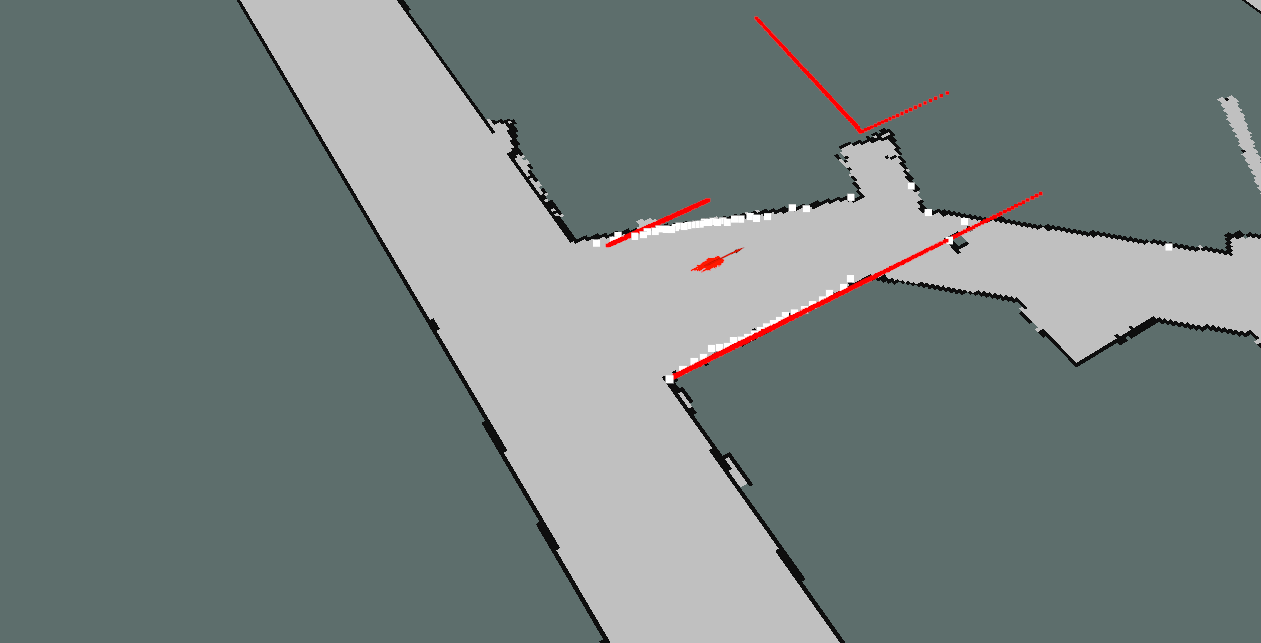
\includegraphics[width=.45\linewidth]{pictures/02/nolocalized}} \quad
  \subfloat[Localized]{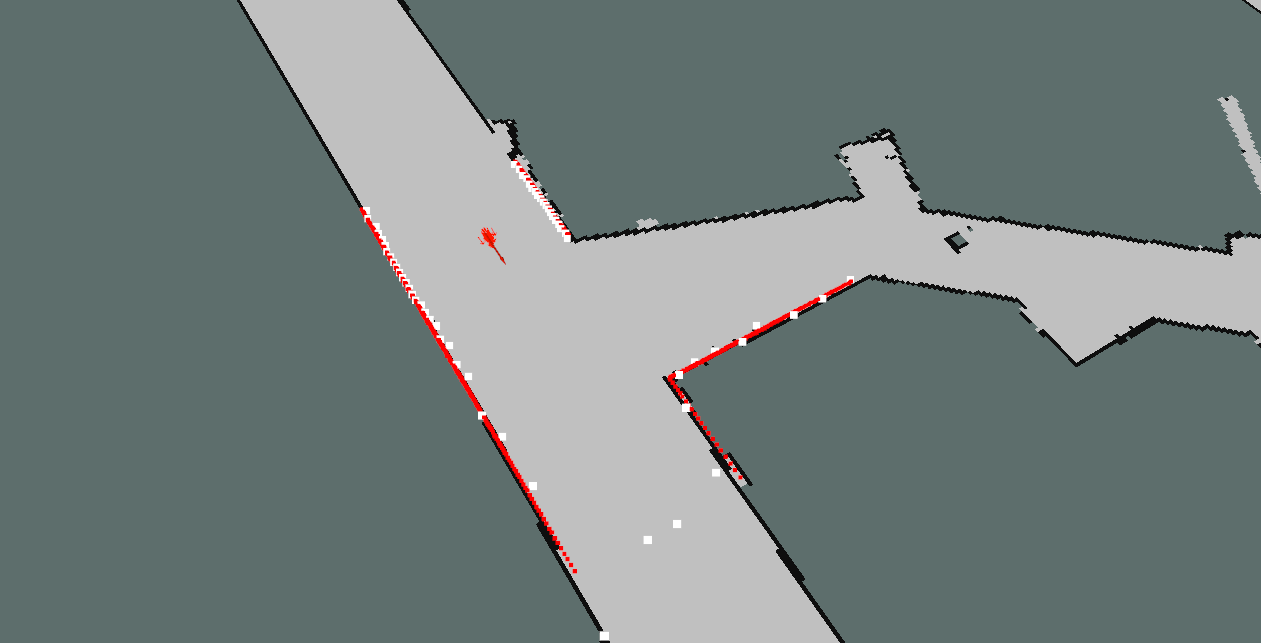
\includegraphics[width=.45\linewidth]{pictures/02/localized}}
  \caption{How probabilistic localization works}
  \label{fig:locnoloc}
\end{figure} 

Those are the most popular algorithms though not unique. Other solutions are landmark--based navigation or route--based navigation. 

\subsection{Planning and Navigation}

Recalling \autoref{fig:control}, it can be inferred that motion planning is the branch that develops algorithms to translate high--level information such maps and human commands into low--level instructions to the controllers \citeauton{LaValle2006}.

Planning and Navigation has 2 goals: reach the desired/commanded location as quickly as possible and avoid obstacles/collisions \citeauton{Burgard2017d}. To achieve that, this task is usually divided in 2 layers as shown in \autoref{fig:plan}.

\begin{figure}[htb]
  \centering
  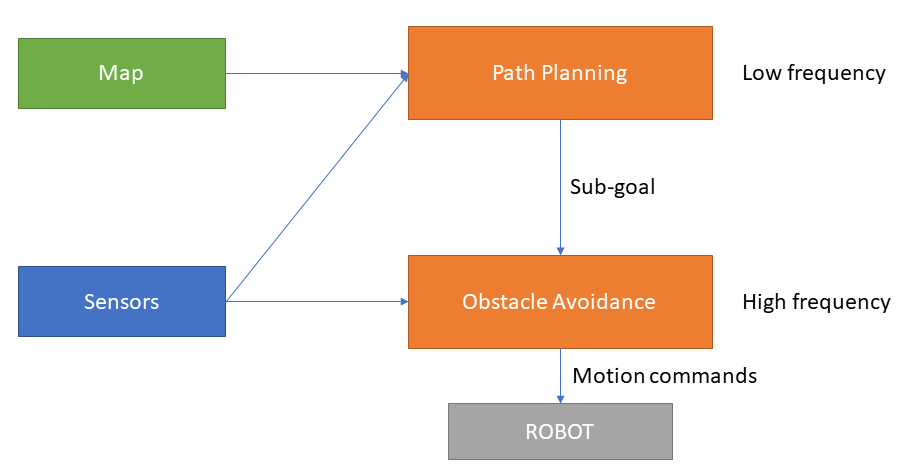
\includegraphics[width=.9\linewidth]{pictures/02/plan}
  \caption{Motion planning workflow}
  \label{fig:plan}
\end{figure} 

\parunder{Path Planning} Path planning can be considered as the long term strategy to reach the goal \citeauton{Siegwart2004}. The objective of this layer is to identify a path that moves to the desired location without hitting any obstacles. For that purpose, the following information is required: The \textbf{start} pose of the robot, the \textbf{goal} pose, the geometrical description of the \textbf{robot} and the representation of the \textbf{environment}. 

The field of path planning was deeply studied for industrial manipulators, and in fact they are more complex cases than differential drive or ackerman steering robots. 

Even though path planning is a real--world problem, when approaching the problem it is often represented in the \textbf{configuration space}, where every state can be represented with k values $q_1, q_2\ldots q_k$, being $k$ the number of degrees of freedom. That space is then discretized and the algorithm is applied. Some of the most common algorithms for path planning are \citeauton{LaValle2006, Burgard2017d}: 
\begin{itemize}
  \item \textbf{Search algorithms}: Such as Dijkstra and A*.

  \item \textbf{Road map planning}: Voronoi diagrams are a very common variety.

  \item \textbf{Cell decomposition}.

  \item \textbf{Rapidly Exploring Random Trees (RRT)}

  \item \textbf{Markov Decision Processes (MDP)}.
\end{itemize}  

\parunder{Obstacle avoidance} Whereas path planning is focused on searching global optimal solutions, obstacle avoidance searches on the local space and modifies the trajectory based on the obstacles detected by sensors. There are many existing algorithms for obstacle avoidance but one of the most utilized (even though there exist more optimal solutions nowadays) is the Dynamic Window Approach (DWA) \citeauton{Fox1997} (\autoref{fig:dwa}).

\begin{figure}[htb]
  \centering
  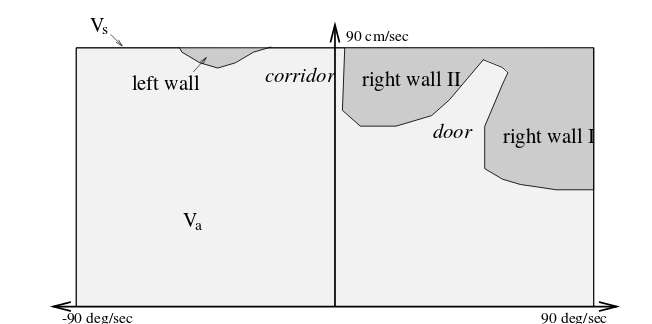
\includegraphics[width=.8\linewidth]{pictures/02/dwa}
  \caption{DWA velocity search space}
  \label{fig:dwa}
\end{figure} 

This algorithm searches the admissible pair of velocities $<v, \omega>$ based on the dynamic constraints and surrounding obstacles that maximize the function:
\begin{equation}
  G(v,\omega)) = \sigma(\alpha\cdot heading(v,\omega)+\beta\cdot dist(v,\omega) + \gamma\cdot vel(v,\omega))
  \label{eq:dwa}
\end{equation}  

where $heading$ measures the distance to the goal (favoring movements towards it), $dist$ the distance to the closest obstacle (favoring clearance) and $vel$ the velocity of the robot (favoring higher speeds).

\section{Robot Operating System (ROS)}

With the rise of robotics, a notable amount of software packages has proliferated these years, either for industrial or research purposes:

\begin{itemize}
  \item \textbf{Industrial robotics software}: Almost every major robot manufacturer ships with their own programming language as it is shown on \autoref{tab:industrial}:

  \begin{table}[htb]
    \centering
    \begin{tabular}{r|l}
      \hline
      \textbf{Company Name} & \textbf{Language Name} \\ \hline
      ABB & \href{https://www.google.com/url?sa=t&rct=j&q=&esrc=s&source=web&cd=1&cad=rja&uact=8&ved=2ahUKEwjFqeGL6e7cAhWHr6QKHS1mBkEQFjAAegQICBAC&url=https%3A%2F%2Flibrary.e.abb.com%2Fpublic%2F688894b98123f87bc1257cc50044e809%2FTechnical%2520reference%2520manual_RAPID_3HAC16581-1_revJ_en.pdf&usg=AOvVaw3zcMHJjAK2YTojeWoqGG_r}{RAPID} \\ \hline
      Kuka & \href{https://drstienecker.com/tech-332/11-the-kuka-robot-programming-language/}{KRL} (Kuka Robot Language) \\ \hline
      Comau & \href{ftp://service.bosso.it/Manuali%20COMAU/IT/handbooks/files/lb-0-0-pdl.pdf}{PDL2} \\ \hline
      Yaskawa & \href{http://spaz.org/~jake/robot/155493-INFORM-LANGUAGE.pdf}{INFORM} \\ \hline
      Fanuc & \href{http://www.onerobotics.com/posts/2013/introduction-to-karel-programming/}{Karel} \\ \hline
    \end{tabular}
    \caption{Industrial robots' programming languages}
    \label{tab:industrial}
  \end{table}

  \item \textbf{Research software}: Some of the libraries used are: Peter Corke's Robotic Toolbox for Matlab \citeauton{Corke}, \href{https://www.microsoft.com/en-us/download/details.aspx?id=29081}{Microsoft Robotics Developer Studio}, \href{https://www.roboticslibrary.org/}{Robotics Library} and many others.
\end{itemize} 

These are not the only items available, in fact the field of robotics is too broad, and there is no perfect solution that covers all the aspects of the it. However, there is one tool that is very popular among researchers and companies around the world and that is called \href{http://www.ros.org/}{Robot Operating System (ROS)}.

\subsection{Why and what is it?}

Every year, robotics grows in size and scaling software becomes a daunting challenge \citeauton{Quigley2009}. This is because robotics gathers the fields of Mechanical and Electrical Engineering with Computer Science, thus software must contain driver level software up to perception and higher levels of abstraction.

Since very few researchers have sufficient knowledge on all the aspects mentioned above, code reuse is a must of any robotics software.

Therefore, in 2008, researchers from Stanford University, University of Southern California (UCSC) and Willow Garage began developing ROS as a continuation of previous software packages such as Stanford's STAIR \citeauton{Quigley2007} and Willow Garage's Personal Robots Program \citeauton{Wyrobek2008}. ROS continued to grow and in 2014, the Open-Source Robotics Foundation (OSRF) took charge of the development and maintenance of the ecosystem\footnote{For more on the history of ROS: \url{http://www.ros.org/history/}}.

ROS was built with the following design goals in mind \citeauton{Quigley2009, Quigley2015} (Figure \autoref{fig:ros} shows a representation of those concepts):

\begin{figure}[htb]
  \centering
  
\includegraphics[width=\linewidth]{pictures/02/ros_equation}
  \caption{Capabilities of ROS}
  \label{fig:ros}
\end{figure}

\begin{itemize}
  \item \textbf{Peer to peer}: ROS consists on different processes that run in a peer--to-peer network exchanging information between them. This way several machines can be attached, performing each one different tasks. For instance, a robot can have several onboard machines sensing and sending actuation commands via ethernet, while offboard machines connected to the previous ones wirelessly can take charge of 'heavier' tasks such as SLAM or Computer Vision (\autoref{fig:peer}).

  \begin{figure}[htb]
    \centering
    % 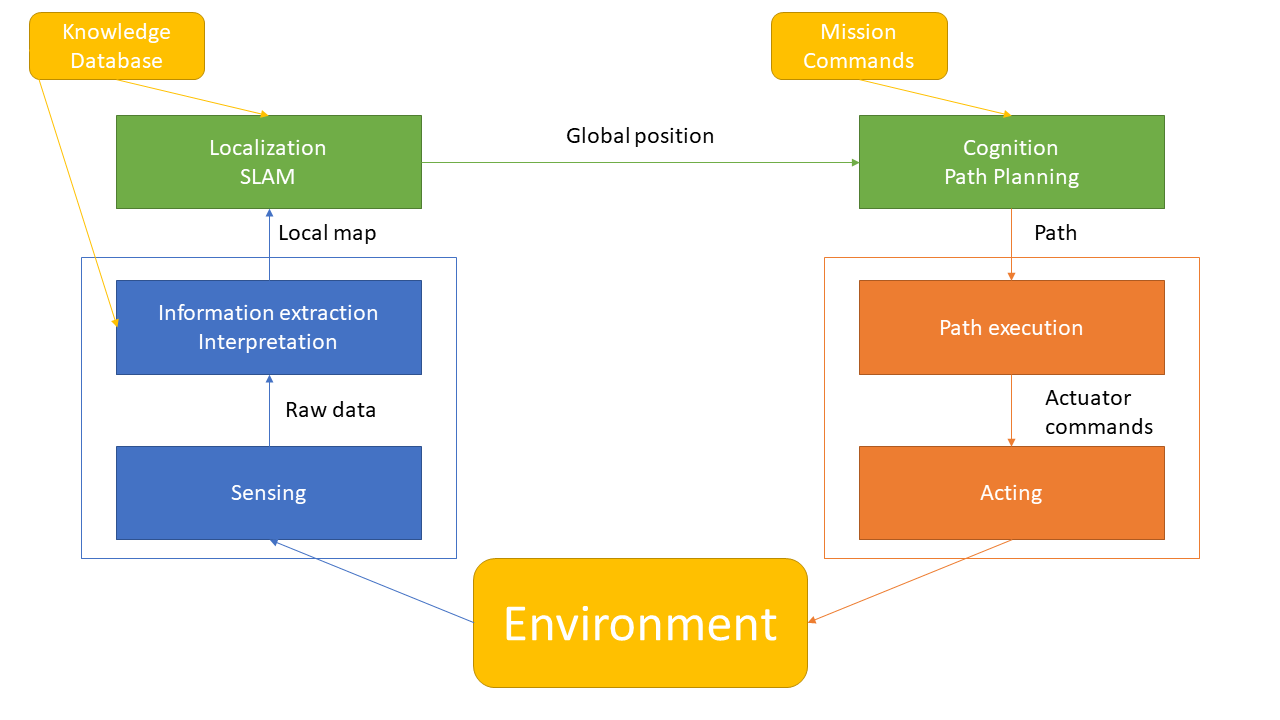
\includegraphics[width=\linewidth]{pictures/02/control}
    \caption{Schematic of the networking capabilities of ROS}
    \label{fig:peer}
  \end{figure}

  \item \textbf{Tools based}: Instead of an enormous standalone application, ROS is composed of several tools with various functionalities, such as navigating the structure, visualizing sensor inputs, compiling, and many others.

  \item \textbf{Multi-lingual}: As every programming language excels at different tasks, ROS provides client libraries for a great variety of languages \footnote{\url{http://wiki.ros.org/Client Libraries}}, being the main ones C++, Python and LISP

  \item \textbf{Thin}: ROS conventions encourage developers to create standalone algorithms and drivers in order to promote code reuse. Those software packages can then be wrapped around ROS and be used on the netowork.

  \item \textbf{Free and Open-Source}: ROS full source is publicly available and anyone can make contributions to its core. This core is licensed under BSD, thus allowing for either commercial or non commercial use.Individual modules or components can have their own licensing.
\end{itemize}

In a more formal definition, ROS is an open-source framework that includes a collection of tools, libraries and conventions to allow for robotic system development \citeauton{Quigley2015}. 

\subsection{Structure of ROS}

\parunder{Basic Concepts} The structure of ROS is composed of \textbf{nodes}, \textbf{messages}, \textbf{topics} and \textbf{services} \citeauton{Quigley2009, OKane2013}:

\begin{itemize}
  \item \textbf{Nodes}: They are the equivalent of software modules and perform one specific computation. When running an application built on ROS, it will very often be composed of several nodes communicating with each other.

  \item \textbf{Messages}: They are data structures that nodes use to communicate. Messages can be composed of basic types or other messages as shown on \autoref{lst:messages}, where a first file \texttt{point.msg} is created to contain 2 variables referring to the position of an object, and the second one \texttt{points.msg} will store a vector of those points:
  \begin{lstlisting}[float=htb,language=Python,frame=htb,caption={Example message files},label=lst:messages] 
    # First file: point.msg
    float32 x
    float32 y 
    # Second file: pointarray.msg
    std_msgs/header header
    point[] points
  \end{lstlisting}

  \item \textbf{Topics}: They act as the containers for the messages. A single node can \textit{publish} messages to a variety of topics, so that other nodes can \textit{subscribe} to one or more of those topics and perform their computations. Topic names must always start with "/" (\ie  "/topic\_name").

  \item \textbf{Services}: Topics can be read/written by any node and sometimes a more bidirectional form of communication is wanted between 2 nodes, in a similar fashion as web services employ request and response documents. That is why services exist (\autoref{lst:services}).
  \begin{lstlisting}[float=htb,language=Python,frame=htb,caption={Example service file},label=lst:services] 
    # File: myService.srv
    # Here goes the request
    int32 x
    int32 y
    ---
    # Here goes the response
    bool success
    int32 multiplication
  \end{lstlisting}
\end{itemize}  

When many nodes and topics are running at the same time, debugging might become difficult. That is why ROS provides a tool called \texttt{rqt\_graph}, in order to visualize all dependencies among processes (\autoref{fig:graph}).
\begin{figure}[htb]
  \centering
  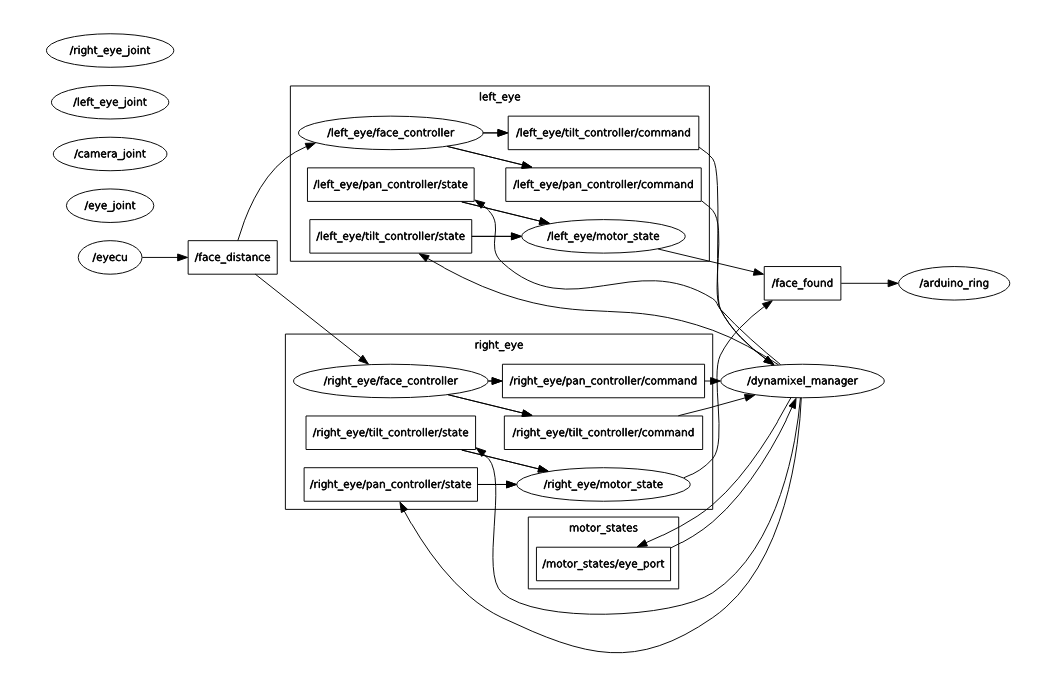
\includegraphics[width=\linewidth]{pictures/02/graph}
  \caption[ROS graph example]{ROS graph example. The flow is represented as: nodes (circles) send messages (arrows) to topics (boxes)}
  \label{fig:graph}
\end{figure}

\parunder{Build system} ROS is packaged with several tools to produce libraries, executables and scripts in both C++ and Python (and other languages with a little tweaking) \citeauton{Quigley2015}. The key concepts here are: \textbf{packages}, \textbf{workspaces} and \textbf{catkin}:

\begin{itemize}
  \item \textbf{Packages}: In ROS, all software, data and documentation is organized into packages. Packages are organized in folders (source code in \texttt{src/}, message files in \texttt{msg/}, launch files in \texttt{launch/}) and need to have 2 files, \texttt{CMakeLists.txt} and \texttt{package.xml} with instructions for the build tools.

  \item \textbf{Workspaces}: Packages are bundled in directories called workspaces, that by convention are called \texttt{exampleworkspace\_ws}. \autoref{fig:ws} shows the structure of workspaces, where packages must be located in the \texttt{src/} folder, and the \texttt{install/} and \texttt{devel/} directories contain the executables and libraries.

  \begin{figure}[htb]
    \centering
    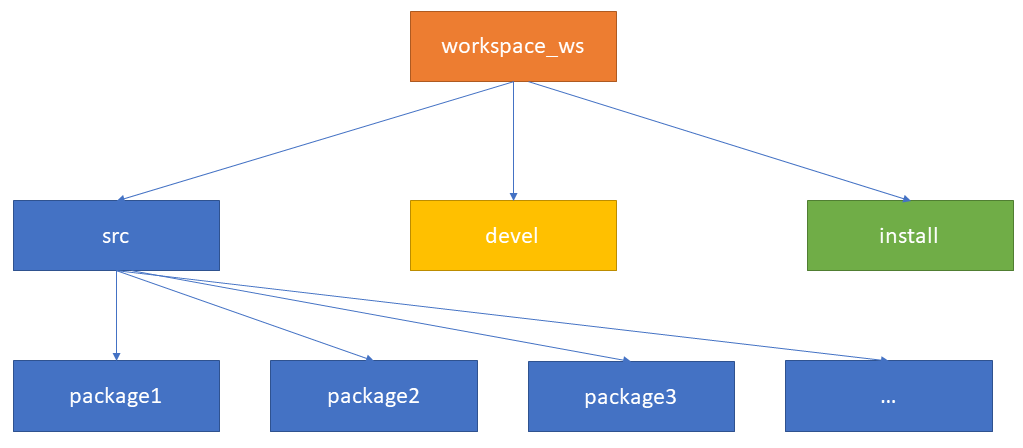
\includegraphics[width=.8\linewidth]{pictures/02/ws}
    \caption{Workspace structure}
    \label{fig:ws}
  \end{figure}

  \item \textbf{Catkin}: It is the offitial build system for ROS. More specifically, it defines some macros and Python scripts to extend the capabilities of CMake, so that building ROS packages is easier \footnote{More information on: \url{http://wiki.ros.org/catkin/conceptual_overview}}. 
\end{itemize}

In order to create the executables, ROS provides the tool \texttt{catkin\_make} and it is used as shown in \autoref{lst:catkin}:
\begin{lstlisting}[float=htb,language=bash,frame=htb,caption={Use of catkin\_make},label=lst:catkin] 
  # Go to workspace
  user@host:~$ cd workspace_ws 
  # Compile packages
  user@host:~/wokspace_ws$ catkin_make 
  # If no errors appear
  user@host:~/wokspace_ws$ source devel/setup.bash
  # This way other ROS tools can find the executables
\end{lstlisting}

\parunder{Running the system} To start any ROS session, there are 3 major components: \textbf{roscore}, \textbf{rosrun} and \textbf{roslaunch}:
\begin{itemize}
  \item \textbf{roscore}: This command launches the ROS master, which is in charge of providing nodes with information to establish communication with other nodes. If the core is not running, nodes cannot find each other and ROS will not start.

  \item \textbf{rosrun}: It searches for the specified node in the specified package and starts it: \texttt{rosrun <package> <executable> <arguments>}.

  \item \textbf{roslaunch}: When the number of nodes and parameters grows in size, it is possible to group several nodes in an \texttt{.xml} file and run them with the \texttt{roslaunch} command (\autoref{lst:roslaunch}). 
  \begin{lstlisting}[float=htb,language=xml,frame=htb,caption={Example of launch file},label=lst:roslaunch] 
    <launch>
    <!-- Node to launch necessary files from Jetson -->

      <!-- Launch hackbike serial -->
      <node pkg="hackbike" type="hackbike_serial" name="hackbike_serial_node" output="screen"/>

      <arg name="mode" default="pedestrian"/>

      <!-- Launch data sender node -->
      <param name="mode" value="$(arg mode)"/>
      <node pkg="panasonic" type="send_data_to_bike.py" name="data_sender_node" output="screen"/>

      <!-- Start tensorflow node -->
      <arg name="tensorflow" default="false"/>
      <group if="$(arg tensorflow)">
        <include file="$(find panasonic)/launch/start_tensorflow.launch"/>
      </group>

      <include file="$(find panasonic)/launch/start_arduino.launch"/>

    </launch>
  \end{lstlisting}
\end{itemize}  

\parunder{Visualization and simulation} It has already been stated that ROS is a tools-based platform, and 2 of those main tools are \textbf{RViz} and \textbf{Gazebo}:

\begin{itemize}
  \item \textbf{RViz}: It is the standard visualization tool for ROS, capable of rendering 3D models, sensed images and pointclouds \citeauton{Gossow2011}. It is widely used for controlling robotic systems based on ROS (\autoref{fig:rviz})
  \begin{figure}[htb]
    \centering
    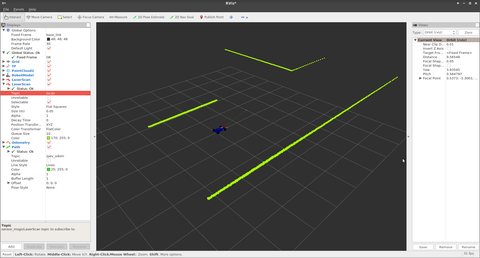
\includegraphics[width=.9\linewidth]{pictures/02/rviz}
    \caption{RViz showing the points received by a LiDAR}
    \label{fig:rviz}
  \end{figure}  

  \item \textbf{Gazebo}: It is an open--source robot simulator with support for multiple robots in complex environments \citeauton{Koenig2004}. It is a different platform from ROS, but they can be bundled together (\autoref{fig:gazebo}).
  \begin{figure}[htb]
    \centering
    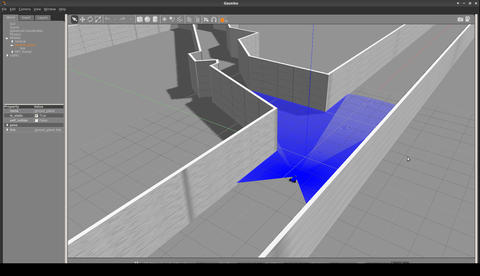
\includegraphics[width=.9\linewidth]{pictures/02/gazebo}
    \caption{Small robot in Gazebo}
    \label{fig:gazebo}
  \end{figure}  
\end{itemize}  

\subsection{Navigation stack}

ROS provides a collection of packages that allow for 2D indoor navigation called Navigation Stack \citeauton{Marder2010}. Basically, this framework reads odometry, laser data and transforms and outputs velocity commands to the controllers. \autoref{fig:navistack} shows a conceptual map of the Navigation Stack. 
\begin{figure}[htb]
  \centering
  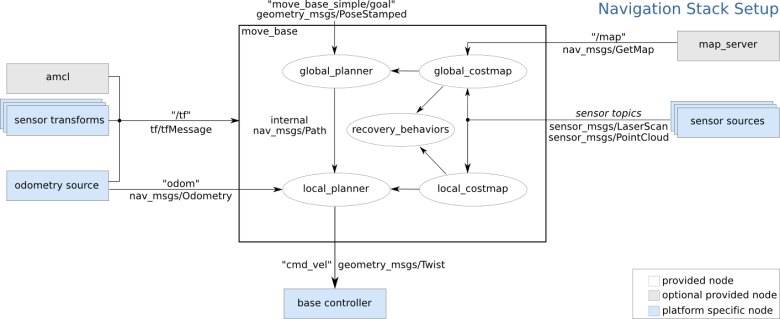
\includegraphics[width=\linewidth]{pictures/02/navistack}
  \caption{Navigation Stack overview}
  \label{fig:navistack}
\end{figure}  

The main nodes provided by the stack are:

\begin{itemize}
  \item \textbf{Global costmap}: It reads the information of a static map and creates a 2D layer with the obstacles detected in it. This layer will remain mostly unchanged. 

  \item \textbf{Local costmap}: It creates a smaller 2D costmap with the available laser data that gets updated frequently in order to account for dynamic obstacles.
  
  \item \textbf{Global planner}: With the information from the global costmap and a desired goal, it provides a high-level plan for the robot to follow. It uses algorithms like Dijkstra or A* and it does not take into account any kinematic or dynamic restrictions.

  \item \textbf{Local planner}: It reads the global plan and the local costmap and outputs velocity commands that follow the global plan as closely as possible while avoiding obstacles. This planner takes into account the constraints the robot might have.
\end{itemize}  

The navigation stack is a useful tool but has its limitations as well. First, it is optimized for 2D navigation which is less accurate and not particularly suitable for large environments. Second, it was designed for indoor navigation not for outdoor scenarios. And third, it only considers differential and holonomic drive robots.

However, it is possible to modify some of the nodes provided to extend the functionalities of the stack, as it has been done with the PEV.
 % Chapter 2
\cleardoublepage % Empty page before the start of the next part

% Description of slam, common approaches and frameworks

\chapter{Simultaneous Localization and Mapping (SLAM)}
\label{ch:slam}

Simultaneous Localization and Mapping (\textbf{SLAM}) or Concurrent Mapping and Localization (\textbf{CML}) is one of the most fundamental problems in robotics \citeslam{Durrant-Whyte2006, Thrun2005, Tobergte2013}. It tackles the task of placing a robot in an unknown environment and being able to build a map while keeping track of the robot's own position on that map.

Since SLAM is one of the core features of mobile robotics, its applications range in the same field such as ground, indoor, underwater or air vehicles (\autoref {fig:slam}).
\begin{figure}[htb]
  \centering
  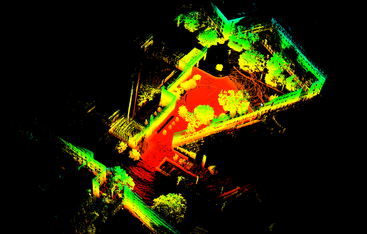
\includegraphics[width=\linewidth]{pictures/03/3dslam}
  \caption{3D example of SLAM techniques on the PEV}
  \label{fig:slam}
\end{figure}  


For its nature, SLAM is considered to be one of the toughest challenges of mobile robotics \citeslam{Burgard2017e, Thrun2005} and it is often referred as a \textbf{chicken--and--egg} problem:
\begin{itemize}
  \item In order for a robot to correct errors from odometry and localize in the environment it needs a map.

  \item In order to build a map, the robot needs to know its position and orientation with respect to the environment.
\end{itemize}

This interdependence between both problems is why they have to be approached at the same time, thus being named 'Simultaneous'.

SLAM is seen as the 'holy grail' of AVs and mobile robots in general \citeslam{Durrant-Whyte2006}, since once a robust method of building rich maps is found, it will allow for fully autonomous vehicles.

In fact, the SLAM problem has been solved in the theoretical plane, where many equally valid variants can be found; the problem arises when those algorithms are applied in real--life systems.

\section{SLAM fundamentals}

\subsection{Probabilistic Robotics}

The approach to SLAM is generally done in terms of probability instead of using single "best guess" values. This manner of tackling SLAM (and many other fields in mobile robotics) results to be very useful since neither sensors nor actuators are noise--free. By integrating those uncertainties into the models, controls can be made more robust, thus improving the performance of the robot.

The core of probabilistic robotics is \textbf{state estimation}, that is estimating environment and internal variables using sensor data. 

Denoting time with letter $t$, the state and environmental variables can be defined as \citeslam{Thrun2005, Tobergte2013}:
\begin{itemize}
  \item \textbf{State}: State is usually denoted with letter $x$ and is composed of position and orientation (relative to global frame), more commonly called \textbf{pose}. In flat navigation, the state comprises the tuple $(x\,\,y\,\,\theta)$. Thus, the state at time $t$ is denoted as $x_t$, and the collection of states from time $0$ to $t$, namely the \textbf{path}, is:
  \begin{equation}
    X_t = \{x_0, x_1, x_2,\ldots,x_t \}
    \label{eq:state}
  \end{equation} 

  Moreover, states can be \emph{complete} or \emph{incomplete}. A state is called \emph{complete} when the prior knowledge of state, control and perception does not add more information. However, in real--life situations, not all aspects of the robot are known, being that called \emph{incomplete}.

  % Mention chapter 2
  \item \textbf{Control actions}: Control actions change the state of the system (\eg, manipulation, forward movement) and data associated to these actions contain information on how the state changes. One of the most common sources of data is \emph{odometry} (\autoref{sub:perception}). Even though the sources of odometry are sensors, they measure the change of state, being equally valid for the purpose.
  
  Control data is usually denoted with $u$, and $u_t$ denotes the action that brings the system from state $x_{t-1}$ to $x_t$. Actions are collected in the vector:
  \begin{equation}
    U_t = \{u_0, u_1, u_2,\ldots,u_t \}
    \label{eq:actions}
  \end{equation}   

  \item \textbf{Environment measurements}: Sensors such as lidars or camera perform \emph{observations} to gain knowledge of the state of the system. Measurement data is denoted with $z$ and $z_t$ corresponds to a specific measurement at time $t$. $Z_t$ will denote the collection of all measurements from $0$ 0 to $t$:
  \begin{equation}
    Z_t = \{z_0, z_1, z_2,\ldots,z_t \}
    \label{eq:env}
  \end{equation}  
\end{itemize}  

Once the main variables have been defined, they are usually gathered into a probability distribution called \emph{belief} or \emph{state of knowledge}, that represents the pose at time $t$ taking into account the previous data:
\begin{equation}
  bel(x_t) = p(x_t|z_{1:t},u_{1:t})
  \label{eq:belief}
\end{equation}  

There is a variant of the belief, called prediction, that estimates the pose without taking into account the latest sensor measurement and that is denoted $\overline{bel}(x_t)$:
\begin{equation}
  \overline{bel}(x_t) = p(x_t|z_{1:t-1},u_{1:t})
  \label{eq:prediction}
\end{equation}  

Having defined these variables, now the Bayes filter can be deduced.

\subsection{Bayes filter}

The bayes filter is a technique to peform state estimation, based on previous beliefs and sensor measurements. It is of essential importance in Probabilistic Robotics, since it is the basis for practically all other approaches in the field \citeslam{Burgard2017e, Durrant-Whyte2006}.

The goal is to determine the law that provides the probability distribution of the belief at time $t$, $bel(x_t)=p(x_t|z_{1:t},u_{1:t})$. For that we start with the combined probability $p(x_t,z_{1:t},u_{1:t})$ and apply the \textbf{Bayes rule} (hence the name):

\begin{equation}
  \begin{split}
    p(x_t,z_{1:t},u_{1:t}) & = p(z_{1:t-1},u_{1:t})\cdot p(z_t|z_{1:t-1},u_{1:t})\cdot p(x_t|z_{1:t},u_{1:t})\\
                           & = p(z_{1:t-1},u_{1:t})\cdot p(x_t|z_{1:t-1},u_{1:t})\cdot p(z_t|x_t,z_{1:t-1},u_t)
  \end{split}  
  \label{eq:bayesded}
\end{equation}  

Considering that $p(z_{1:t-1},u_{1:t})$ appears on both sides, it can be cancelled out. Then, reordering the elements of the equation:
\begin{equation}
  \begin{split}
    bel(x_t) = p(x_t|z_{1:t},u_{1:t}) & = \frac{p(z_t|x_t,z_{1:t-1},u_t)\cdot p(x_t|z_{1:t-1},u_{1:t})}{p(z_t|z_{1:t-1},u_{1:t})} \\ 
                                      & = \eta\cdot p(z_t|x_t,z_{1:t-1},u_t)\cdot \overline{bel}(x_t)
  \end{split}
  \label{eq:bayes}
\end{equation} 

Where parameter $\eta$ is called \emph{normalizer}. If it is assumed that the state is complete, then the measurement $z_t$ does not depend on the previous measurements or controls (this is called \textbf{Markov assumption}), thus it can be written:
\begin{equation}
  p(z_t|x_t,z_{1:t-1},u_t) = p(z_t|x_t)
  \label{eq:markovf}
\end{equation}  

As for the prediction, $\overline{bel}(x_t)$, applying the \emph{Theorem of Total Probability} the following is obtained:
\begin{equation}
  \begin{split}
    \overline{bel}(x_t) & = p(x_t|z_{1:t-1},u_{1:t})\\
                        & = \int p(x_t|x_{t-1},z_{1:t-1},u_{1:t})\cdot p(x_{t-1}|z_{1:t-1},u_{1:t})\cdot\mathrm{d}x_{t-1}
  \end{split}
  \label{eq:predicteq}  
\end{equation}  

Applying again the Markov assumption to $ p(x_t|x_{t-1},z_{1:t-1},u_{1:t})$, the resulting probability distribution is ($u_t$ is not cancelled since it carries information on the change from $x_{t-1}$ to $x_t$):
\begin{equation}
  p(x_t|x_{t-1},z_{1:t-1},u_{1:t}) = p(x_t|x_{t-1},u_t)
  \label{eq:markovs}
\end{equation}

As for the second term, $u_t$ can be taken away, as it does not predict state $x_{t-1}$:
\begin{equation}
  p(x_{t-1}|z_{1:t-1},u_{1:t}) = p(x_{t-1}|z_{1:t-1},u_{1:t-1}) = bel(x_{t-1})
  \label{eq:beliefprev}
\end{equation}

After these changes, \autoref{eq:bayes} is converted to:
\begin{equation}
  \begin{split}
    bel(x_t) & = \eta\cdot p(z_t|x_t)\cdot \overline{bel}(x_t)\\
                        & = \eta\cdot p(z_t|x_t)\cdot \int p(x_t|x_{t-1},u_t)\cdot bel(x_{t-1})\cdot\mathrm{d}x_{t-1}
  \end{split}
  \label{eq:bayesfinal}  
\end{equation} 

There are 2 important components in \autoref{eq:bayesfinal}, namely the \emph{measurement probability} $p(z_t|x_t)$, and the \emph{state transition probability} $p(x_t|x_{t-1},u_t)$. In \citeslam{Thrun2005}, \emph{observation models} and \emph{motion models} are provided, that allow to describe those probability distributions more accurately (\autoref{fig:bayesfilter}).
\begin{figure}[htb]
  \centering
  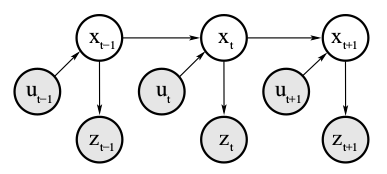
\includegraphics[width=\linewidth]{pictures/03/bayesfilter}
  \caption{Schematic of state determination using Bayes filter}
  \label{fig:bayesfilter}
\end{figure}

\subsection{Probabilistic robotics in SLAM}

When tackling SLAM, there is another variable that needs to be defined and it corresponds to the map features $m_i$, being $m$ the set of the $n$ features that compose the \textbf{map}:
\begin{equation}
  m = \{m_1,m_2,\ldots,m_n\}
  \label{eq:mapvar}
\end{equation}  

It is possible to add the map to the Bayes filter (\autoref{eq:bayesfinal}), since it can be considered as an extension of the state of the system. Therefore the bayes filter becomes:
\begin{equation}
  p(x_t,m|z_{1:t},u_{1:t}) = \eta\cdot p(z_t|x_t,m)\cdot p(x_t,m|z_{1:t-1},u_{1:t})
  \label{eq:bayesslam}  
\end{equation} 

In the probabilistic realm, there are 2 main forms of SLAM (\autoref{fig:approachslam}):
\begin{itemize}
  \item \textbf{Online SLAM}: This approach only seeks to recover the most recent pose and map as it is stated in \autoref{eq:bayesslam}. The previous poses and measurements get discarded in this approach.
  
  \item \textbf{Full SLAM}: In this case, instead of the current position, the whole path is estimated, yielding the following equation:
  \begin{equation}
    p(x_{0:t},m|z_{1:t},u_{1:t})
    \label{eq:fullslam}
  \end{equation}

  It is possible to derive the online SLAM from the full SLAM, by integrating all the poses throughout time \citeslam{Burgard2017e}:
  \begin{equation}
    p(x_t,m|z_{1:t},u_{1:t}) = \int\int\!\cdots\!\int p(x_{1:t},m|z_{1:t},u_{1:t})\mathrm{d}x_1\mathrm{d}x_2\ldots\mathrm{d}x_{t-1}
    \label{eq:onlinetofull}
  \end{equation}
\end{itemize}

\begin{figure}[htb]
  \centering
  \subfloat[Online SLAM]{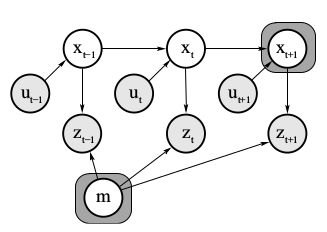
\includegraphics[width=.45\linewidth]{pictures/03/onlineslam}} \quad
  \subfloat[Full SLAM]{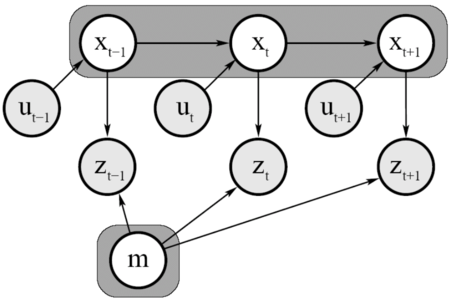
\includegraphics[width=.45\linewidth]{pictures/03/fullslam}}
  \caption{Schematic of the 2 SLAM approaches}
  \label{fig:approachslam}
\end{figure}

\subsection{SLAM dimensions}

The most usual differences among the SLAM algorithms are defined in the following paragraphs \citeslam{Tobergte2013}:

\begin{itemize}
  \item \textbf{Volumetric/Feature--based}: In volumetric SLAM, the map is sampled at realistic resolutions, thus the computational complexity grows notably. In feature--based maps, there are algorithms that process sensor readings and extract the key landmarks of the environment. The latter group is more data efficient, but it may lose some important sensor information.

  \item \textbf{Topological/Metric}: Topological maps are those that only characterize the environment with basic relationships, whereas metric ones provide more accurate descriptions of the surroundings (\autoref{fig:topometric}).
  \begin{figure}[htb]
    \centering
    \subfloat[Topological]{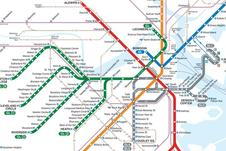
\includegraphics[width=.45\linewidth]{pictures/03/bsubway}} \quad
    \subfloat[Metric]{\includegraphics[width=.45\linewidth]{pictures/03/breal}}
    \caption[2 maps of Boston]{2 maps of Boston: Subway (Topological) vs Satellite (Metric)}
    \label{fig:topometric}
  \end{figure}
  

  \item \textbf{Known/Unknown correspondence}: Correspondence refers to matching sensed features from different timestamps. Some SLAM algorithms assume the identity of landmarks is known while others do not. The problem of determining those correspondences is known as \emph{data association} and it is one of the toughest challenges in SLAM.

  \item \textbf{Static/Dynamic}: The same way as it was described in localization (\autoref{sub:localization}), environments can be static if the environment remains the same over time, or dynamic if there are moving parts. Most of SLAM algorithms suppose static worlds.

  \item \textbf{Small/Large uncertainty}: Algorithms that allow for small uncertainties require that robots move along simple paths back and forth. If the path is more complex and there are multiple paths to return to the starting point, it will cause more uncertainty. In these cases the ability of the algorithm to perform \textbf{loop closure} correctly is crutial. Loop closure is the task of matching a previously visirted area with the current sensor readings \citeslam{Newman2005}. Today, most SLAM algorithms implement more or less sophisticated loop--closing modules. 

  \item \textbf{Active/Passive}: As in localization, when the SLAM algorithm is passive, it just observes to the movement of the robots and estimates the location and the map. In active SLAM, the algorithm itself takes control of the vehicle, resulting in more accurate maps. Nevertheless, the majority of SLAM approaches belong to the passive field.

  \item \textbf{Single/Multi--robot}: Most approaches use the single--robot assumption, though the multi--robot exploration is gaining adepts in the last years. In the latter form, robots are given relative positions to each other and a form of communication among them.
\end{itemize}

\section{SLAM varieties} \label{sec:varieties}

Having set the basics of the SLAM problem, it is time to describe the 3 main SLAM paradigms from which most of the algorithms stem: \textbf{Kalman filter SLAM}, \textbf{Particle filter SLAM} and \textbf{GraphSLAM}.

\subsection{Kalman Filter SLAM} \label{sub:ekf}

Kalman filter SLAM (more specifically Extended Kalman Filter (EKF)) is one of the earliest versions of SLAM \citeslam{Thrun2005,Tobergte2013}. As its name suggests it is based on Kalman filter approaches, which are methods devised by R.E. Kalman in the 1960s to solve the discrete linear filtering problem \citeslam{Bishop2001}. 

Kalman filter and its siblings assume that states can be modelled by gaussian distributions \citeslam{Stachniss2014a}:
\begin{equation}
  p(x) = det(2\pi\Sigma)^{-\frac{1}{2}}\cdot exp({-\frac{1}{2}(x-\mu)^T\Sigma^{-1}(x-\mu)})
  \label{eq:gauss}
\end{equation}  

Where $x$ is the state vector, $\mu$ is the mean vector and $\Sigma$ is the covariance matrix.

Kalman filter then models the state prediction and the measurement as:
\begin{gather}
  x_t = A_tx_{t-1} + B_tu_t + \epsilon_t \\
  z_t = C_tx_t + \delta_t 
  \label{eq:kfpred}
\end{gather}  
where $A_t$ is a $(n\times n)$ matrix that describes the evolution from $t-1$ to $t$ without controls, $B_t$ is a $(n\times l)$ matrix that describes the changes induced by control $u_t$, $C_t$ a $(k\times n)$ matrix that maps the state to the observations and $\epsilon_t,\delta_t$ are zero--mean random variables representing the noise in controls and measurements.

The filter described in \autoref{eq:kfpred} is only valid for linear systems, which is not the case in many real life environments \citeslam{Bishop2001, Stachniss2014b}. Instead, the EKF supposes non linear functions that map the prediction and measurement:
\begin{gather}
  x_t = g(x_{t-1},u_t) + \epsilon_t \\
  z_t = h(x_t) + \delta_t
  \label{eq:ekf}
\end{gather}

Functions $g$ and $h$ are then linearized via Taylor expansion around the mean of $x_{t-1}$ to calculate the posterior:
\begin{gather}
  g(x_{t-1},u_t) \approx g(\mu_{t-1},u_t) + \frac{\partial g(\mu_{t-1},u_t)}{\partial x_{t-1}}(x_{t-1}-\mu_{t-1})\\ 
  h(x_t) \approx h(\overline{\mu}_t) +  \frac{\partial h(\overline{\mu}_t)}{\partial x_t}(x_t - \overline{\mu}_t) 
  \label{eq:taylor}
\end{gather} 

When it comes to EKF SLAM, maps are \emph{feature based}, that is, composed of a collection of landmarks. The robot state estimation is the \emph{combined} state of $x_t$ and the coordinates of the landmarks, $m$:
\begin{equation}
  \begin{split}
    y_t & = \begin{pmatrix} x_t \\ m \end{pmatrix} \\
        & = (x\; y\; \theta\; m_{1,x}\; m_{1,y}\; m_{2,x}\; m_{2,y}\; \ldots\; m_{N,x}\; m_{N,y})^T
  \end{split}
  \label{eq:combinedstate}
\end{equation}  
where $\mu_t$ is a $2N+3$ size vector representing the mean at time $t$ and $\Sigma_t$ is a $2N+3$ matrix that describes the covariance matrix.

The filter cycle of the algorithm is the following \citeslam{Stachniss2014b}: \begin{enumerate*} \item State prediction, \item Measurement prediction, \item Measurement, \item Data association and \item State update.\end{enumerate*}
 

EKF SLAM has been applied successfully in many environments from underwater to aerial spaces. \autoref{fig:ekfslam} shows an example of the application of EKF SLAM using 8 landmarks. From a) to c) the robot pose uncertainty grows until it detects the first feature again and the pose uncertainty decreases.

\begin{figure}[t]
  \centering
  \includegraphics[width=.9\linewidth]{pictures/03/ekf}
  \caption{EKF SLAM example}
  \label{fig:ekfslam}
\end{figure} 

However, it has its drawbacks. Due to the nature of the covariance matrix, every update step takes a quadratic time, thus making the feature number low (less than 1000 features) \citeslam{Thrun2005}.

Because the number of features needs to remain low, \emph{data association} tends to become more difficult. Data association is matching the most likely measurement to a specific landmark. EKF is generally more fragile to other methods to incorrect data associations. Therefore EKF SLAM algorithms are not particularly scalable to larger problems.

Modern EKF algorithms implement some features to avoid the issues of the earliest approaches. Furthermore, there is another approach called \textbf{Extended Information Filter (EIF)} described by the information matrix and the information vector \citeslam{Bailey2006b, Stachniss2014c}:
\begin{gather}
  \Omega = \Sigma^{-1} \\
  \zeta = \Sigma^{-1}\mu
  \label{eq:eif}
\end{gather}

This approach is interesting because many of the off--diagonal components of the \emph{normalized} information matrix are $0$, making it a sparse matrix and making update steps more efficient.

\subsection{Particle Filter SLAM} \label{sub:particle}

The particle filter approach seeks to sample the probability distribution with discrete states (known as particles), instead of approximating using Gaussians. Each particle represents the posterior belief of the system and has associated a weight,$w$, that corresponds to the likelihood of that particle \citeslam{Stachniss2014d, Thrun2005}:
\begin{equation}
  \chi_t = \{<x^{[j]},\;w^{[j]}>\}\quad j=1,\ldots,J
  \label{eq:pf}
\end{equation}  

The steps of the particle filter are:
\begin{enumerate}
  \item \textbf{Sample from proposal distribution}: it is represented by letter $\pi$ and in this case it is coincident with the motion model distribution:
  \begin{equation}
    x_t^{[j]} \sim \pi(x_t|\ldots) = p(x_t|x_{1:t-1}, u_t) 
    \label{eq:pfmotion}
  \end{equation}  

  After this step, the predicted particles are obtained, $\overline{\chi}_t$, which is the representation of $\overline{bel}(x_t)$ in the Bayes Filter.

  \item \textbf{Calculate the weights for each particle}: With the particles in $x_t$, the weight of each one is calculated by dividing the target distribution with the proposal wich is proportional to the observation model:
  \begin{equation}
    w_t^{[j]} = \frac{target}{proposal} \propto p(z_t|x_t^{[j]}) 
    \label{eq:pfobs}
  \end{equation}  

  \item \textbf{Resampling}: In this step a sample $i$ is drawn with probability $w_t^{[i]}$ and this process is repeated $J$ times. In this last step, the more likely particles are kept whereas the ones that are more unlikely get discarded.
\end{enumerate}  

The problem of particle filters applied to SLAM is that the state space tends to have a notable size (\autoref{eq:combinedstate}). Particle filters scale exponentially, therefore if the number of landmarks is considerable the problem becomes untractable. 

\textbf{FastSLAM}, originally developed by \citeslam{Montemerlo2002} is an algorithm that exploits the independence among the different map features \autoref{fig:mapindep}. In the original implementation, it only applied to feature based maps.
\begin{figure}[t]
  \centering
  \includegraphics[width=\linewidth]{pictures/03/mapindep}
  \caption[Landmarks are independent from each other]{Conceptual view of how each landmark is disconnected from the rest}
  \label{fig:mapindep}
\end{figure}  

The belief at time $t$ can be factored as:
\begin{equation}
  p(x_{0:t},m|z_{1:t},u_{1:t}) = p(x_{0:t}|z_{1:t},u_{1:t})\cdot \prod\limits_{i=1}^{N}p(m_i|x_{0:t}, z_{1:t})
  \label{eq:rao}
\end{equation}  
where each of the landmarks represents a 2--dimension gaussian distribution with mean and covariance $\mu_{t,n}^{[j]}$ and $\Sigma_{t,n}^{[j]}$ respectively. Due to a technique called \emph{Rao--Blackwellization} for every particle the map posteriors can be estimated independently.

The posterior estimation is done as follows:
\begin{enumerate}
  \item \textbf{Sampling}: A set of particles if sampled from the motion model:
  \begin{equation}
    x_t^{[j]} \sim p(x_t|x_{t-1}^{[j]},u_t)
    \label{eq:slamsamplemotion}
  \end{equation}  

  \item \textbf{Update the observed features estimates}: This is done for each particle and the update is done employing the EKF. For any unobserved feature the gaussian remains the same:
  \begin{equation}
    \langle \mu_{t,n}^{[j]},\; \Sigma_{t,n}^{[j]}\rangle = \langle \mu_{t-1,n}^{[j]},\; \Sigma_{t-1,n}^{[j]}\rangle
    \label{eq:simpleupdate}
  \end{equation}  

  \item \textbf{Resampling}: First the weights are calculated with $p(x_{0:t}|z_{1:t},u_{1:t})$ as target and $p(x_{0:t}|z_{1:t-1},u_{1:t})$ as proposal distributions. Each weight $w_t^{[j]}$ can be obtained via \citeslam{Thrun2005, Tobergte2013}:
  \begin{equation}
    \begin{split}
    w_t^{[j]} & = \frac{target(x^{[j]})}{proposal(x^{[j]})} = \frac{p(x^{[j]}_{0:t}|z_{1:t},u_{1:t})}{p(x^{[j]}_{0:t}|z_{1:t-1},u_{1:t})}\\
              & = \frac{\eta p(z_t|x^{[j]}_{0:t},z_{1:t-1})\cdot p(x^{[j]}_{0:t}|z_{1:t-1},u_{1:t})}{p(x^{[j]}_{0:t}|z_{1:t-1},u_{1:t})} \\
              & = \eta p(z_t|x^{[j]}_{0:t},z_{1:t-1}) \\
              & = \eta\!\int\!  p(z_t|x^{[j]}_{0:t},z_{1:t-1},m_i)\cdot p(m_i|x^{[j]}_{0:t},z_{1:t-1})\cdot \mathrm{d}m_i \\
              & = \eta\!\int\!  p(z_t|x^{[j]}_{0:t},m_i)\cdot p(m_i|x^{[j]}_{0:t},z_{1:t-1})\cdot \mathrm{d}m_i
    \end{split}
  \end{equation}
\end{enumerate}  

Both probability distributions inside the integral can be approximated by Gaussian distributions and the weights can be computed with an EKF. After obtaining the weights for each particle, the new set is created being the particles with bigger weights more likely to 'survive' to the next round.

The FastSLAM algorithm has some notable properties \citeslam{Montemerlo2002, Tobergte2013}: \begin{enumerate*} \item it solves both full and online SLAM problems, \item each particle can make its own data association hypothesis and \item it is possible to implement it very efficiently \end{enumerate*}.

Apart from the feature--based FastSLAM, there exists a Grid--Map based implementation of the algorithm, which is the basis for the \textbf{GMapping} algorithm that will be explained in \autoref{sub:gmapping}.

\subsection{Graph--based SLAM}\label{sub:graphslam}

The last of the approaches that will be discused in this thesis is the \textbf{Graph--based SLAM}. The intuition behind this algorithm is as follows \citeslam{Stachniss2014e}:
\begin{itemize}
  \item \textbf{Graph}: Corresponds to the whole SLAM problem.

  \item \textbf{Nodes}: Correspond to landmarks and robot locations.

  \item \textbf{Edges}: Correspond to spatial constraints due to motion or observations.
\end{itemize}  

The whole purpose of the Graph SLAM is therefore to find a node distribution that minimizes the measurement errors.

Generally, Graph--based SLAM algorithms have the structure shown in \autoref{fig:graphslam}, where the front--end takes the measurements are obtained by \emph{matching} observations, and the backend, where given the measurements it builds the constraints and optimizes the graph.
\begin{figure}[htb]
  \centering
  \includegraphics[width=\linewidth]{pictures/03/graphslam}
  \caption{Graph--based SLAM structure}
  \label{fig:graphslam}
\end{figure}  

\parunder{Backend:} The definition of the optimization is described in the following paragraphs \citeslam{Grisetti2010}. The vector describing the pose of every node $i$ is defined $x = (x_1,x_2,\ldots,x_N)^T$. $z_{ij}$ and $\Omega_{ij}$ are the mean of the measurement and the information matrix from node $i$ to $j$. $\hat{z}_{ij}(x_i,x_j)$ is the prediction of a measurement given nodes $i$ and $j$.

Therefore an error function can be defined as:
\begin{equation}
  e_{ij} = z_{ij} - \hat{z}_{ij}(x_i,x_j)
  \label{eq:error}
\end{equation}  

$\mathbf{F}(x)$ is the negative log likelihood:
\begin{equation}
  \mathbf{F}(x) = \sum\limits_{\langle i,j \rangle}e_{ij}^T\cdot \Omega_{ij}\cdot e_{ij}
  \label{eq:fx}
\end{equation}  
and the objective is to minimize $\mathbf{F}(x)$:
\begin{equation}
  x^* = argmin\;\mathbf{F}(x)
  \label{eq:minfx}
\end{equation}  

\autoref{eq:minfx} corresponds to a \textbf{non--linear least squares} problem and it can be solved using well-known methods such as gradient descent, Newton--Gauss, Lavenberg--Marquardt \citeslam{Grisetti2010}.

Generally, this is done by linearizing the error function with a first order Taylor expansion around the initial guess $\breve{x}$:
\begin{equation}
  \begin{split}
    e_{ij}(\breve{x}_i + \Delta x_i, \breve{x}_j + \Delta x_j) & = e_{ij}(\breve{x} + \Delta x) \\
                                                                & \approx e_{ij} + J_{ij}\Delta x
  \end{split}  
  \label{eq:taylorerror}
\end{equation}
where $J_{ij}$ is the jacobian matrix.

In terms of $F_{ij}$ the equation results in:
\begin{equation}
  \begin{split}
    F_{ij}& (\breve{x}+\Delta x)\\
          & = (e_{ij}(\breve{x} + \Delta x)^T\cdot \Omega_{ij}\cdot e_{ij}(\breve{x} + \Delta x) \\
          & \approx (e_{ij} + J_{ij}\Delta x)^T\cdot \Omega_{ij}\cdot (e_{ij} + J_{ij}\Delta x) \\
          & = e_{ij}^T\Omega_{ij}e_{ij} + 2e_{ij}^TJ_{ij}\Delta x + \Delta x J_{ij}^T \Omega_{ij} J_{ij} \Delta x^T \\
          & = c_{ij} + 2b_{ij}\Delta x + \Delta x^T H_{ij} \Delta x
  \end{split}  
  \label{eq:fij}
\end{equation}

The function $\mathrm{F}(x)$ then becomes:
\begin{equation}
  \begin{split}
    \mathbf{F}(\breve{x}+\Delta x) & = \sum\limits_{\langle i, j \rangle} F_{ij}(x + \Delta x)\\
                                   & \approx \sum\limits_{\langle i, j \rangle} c_{ij} + 2b_{ij}\Delta x + \Delta x^T H_{ij} \Delta x\\
                                   & = \mathbf{c} + 2\mathbf{b}^T\Delta x + \Delta x^T \mathbf{H} \Delta x
  \end{split}  
  \label{eq:fxtaylor}
\end{equation}

\autoref{eq:fxtaylor} can be minimized by solving the linear system:
\begin{equation}
  \mathbf{H}\Delta x^* = -\mathbf{b}
  \label{eq:linearsolve}
\end{equation} 
and therefore the solution becomes:
\begin{equation}
  x^* = \breve{x} + \Delta x^*
  \label{eq:solution}
\end{equation} 

\parunder{Frontend:} The frontend of the Graph--based SLAM obtains the measurements by performing a \textbf{scan--matching} of current sensor data with previous points. The algorithms that tackle this problem are \textbf{Iterative Closest Point (ICP)}, \textbf{Correlative matching}, \textbf{Normal Distributions Transform (NDT)} among many others.

Graph SLAM algorithms have 2 key advantages \citeslam{Tobergte2013} in comparison with EKF SLAM: The update of the map is constant in time and the memory utilization grows linearly. However, the optimization step is resource consuming.

One of the features of these algorithms is that they serve for both 2D and 3D maps \citeslam{Grisetti2010}. The 'only' change that has to be made is to substitute the laser scans with 3D pointclouds. In fact \autoref{fig:slam} was built using a Graph--based SLAM algorithm.

In the past years, Graph SLAM algorithms have been subject to profound research and have become the state--of--the--art algorithms in this field \citeslam{Thrun2005, Tobergte2013}. Some of the biggest SLAM maps have been created using this approach and contain up to 10\textsuperscript{8} features.

\section{Open-source SLAM algorithms}

Fortunately, these algorthms have already been implemented in software packages and many of them are available in the open--source community. What is more, due to the success of the ROS ecosystem, generally SLAM algorithms come bundled with ROS libraries, thus making them easier to interface.

In the following pages, the main algorithms used to develop the SLAM systems of both the Nexus Robot and the PEV will be described.

\subsection{SLAM Gmapping} \label{sub:gmapping}

As it was mentioned on \autoref{sub:particle}, \textbf{Gmapping} is a particle filter SLAM variant that employs grid maps instead of feature--based maps \citeslam{Grisetti2005, Grisetti2007}, that incorporates some improvements to the original algorithms:
\begin{itemize}
  \item \textbf{Scan--matching}: Before applying the particle filter, the pose is corrected using a scan--matcher to maximize the likelihood of the current pose and map:
  \begin{equation}
    x_t^* = \mathop{argmax}_{x_t}\{p(z_t|x_t,m_{t-1})p(x_t|u_t,x^*_{t-1})\}
    \label{eq:scanmatch}
  \end{equation}  

  \item \textbf{Improving the proposal distribution}: Recalling from \autoref{sub:particle}, the importance weights are a result of the ratio between the target distribution $p(x_{0:t}|z_{1:t},u_{1:t})$ and the proposal $\pi(x_{0:t}|z_{1:t},u_{1:t})$. Gmapping computes this proposal taking into account the most recent scan, thus improving accuracy:
  \begin{equation}
    p(x_t|m_{t-1}^{[j]},x^{[j]}_{t-1},z_t,u_{t})=\frac{p(z_t|m_{t-1}^{[j]},x_t)p(x_t|x_{t-1}^{[j]},u_t)}{p(z_t|m_{t-1}^{[j]},x_{t-1}^{[j]},u_t)}
    \label{eq:improvedprop}
  \end{equation}

  \item \textbf{Adaptive resampling}: Even though resampling is necessary since the number of particles is finite and the less likely ones must be removed, the process might also remove good particles. Therefore Gmapping computes the following parameter:
  \begin{equation}
    N_{eff} = \frac{1}{\sum_{i=1}^{N}(\tilde{w}^{[j]})^2}
    \label{eq:neff}
  \end{equation}
  where $\tilde{w}^{(i)}$ is the normalized weight. The algorithm will do a resampling step whenever $N_{eff}$ drops below $N/2$, being $N$ the number of particles. Thus, the resampling operation is done when needed.
\end{itemize}  

Gmapping is one of the first open--source alogorithms to appear on the ROS ecosystem\footnote{http://wiki.ros.org/gmapping} and it blends naturally with the Navigation Stack. Some of the main characteristics of this ROS package are:
\begin{itemize}
  \item \textbf{Subscribed topics}: The main topics are \texttt{/tf} to obtain the rigid body transforms and \texttt{scan} to obtain the laser messages. The necessary transforms are:
  \begin{itemize}
    \item \texttt{laser\_frame}\arrow\texttt{base\_link}. Transformation between the frame of the range sensor and the main frame of the robot.
    \item \texttt{base\_link}\arrow\texttt{odom}. Transformation between the base frame and an odometry frame.
  \end{itemize}  

  \item \textbf{Published topics}: Gmapping publishes the \textbf{occupancy grid map} to the \texttt{/map} topic.

  \item \textbf{Provided transforms}: Gmapping provides the transform \texttt{map}\arrow\texttt{odom} with the robot's pose within the map.

  \item \textbf{Parameters}: \autoref{tab:gmapping} shows a list of the main parameters of the algorithm. The full list can be found on the \href{http://wiki.ros.org/gmapping}{ROS Wiki}
\end{itemize}

\begin{table}[htb]
  \centering
  \resizebox{\textwidth}{!}{%
    \begin{tabular}{lcl}
      \hline
      \textbf{Name} & \textbf{Default} & \textbf{Description} \\ \hline
      $\sim$base\_frame & "base\_link" & Frame attached to mobile base \\ \hline
      $\sim$map\_frame & "map" & Frame attached to the map \\ \hline
      $\sim$odom\_frame & "odom" & Frame attached to odometry \\ \hline
      $\sim$map\_update\_interval & 5 & Time (s) between map updates \\ \hline
      $\sim$maxUrange & 80 & Usable range of the laser \\ \hline
      $\sim$iterations & 5 & Max iterations of the scanmatcher \\ \hline
      $\sim$linearUpdate & 1.0 & Process scan every x meters \\ \hline
      $\sim$angularUpdate & 0.5 & Process scan every x radians \\ \hline
      $\sim$particles & 30 & Number of particles in the filter \\ \hline
      $\sim$resampleThreshold & 0.5 & $N_{eff}$ limit to resample \\ \hline
    \end{tabular}%
  }
  \caption{Gmapping main parameters}
  \label{tab:gmapping}
\end{table} 

\subsection{Hector SLAM} \label{sub:hector}

Hector SLAM is another ROS--based SLAM approach that fully integrates with the Navigation Stack and that is capable of performing 3D motion estimation \citeslam{Kohlbrecher2011}. \autoref{fig:hector} shows the Hector SLAM system overview.
\begin{figure}[htb]
  \centering
  \includegraphics[width=\linewidth]{pictures/03/hector}
  \caption{Hector SLAM overview}
  \label{fig:hector}
\end{figure}  

There are 2 clear layers in the system:
\begin{itemize}
  \item \textbf{SLAM subsystem}: It reads the scans from the laser, performs the scan matching opperation and stores the results on a grid--map in 2 dimensions. This algorithm does not divide the SLAM between frontend and backend as it was explained in \autoref{sub:graphslam}: instead, it relies on the scan--matching operation to update the map. Maps are divided into multiple resolution layers to gain more consistency in the localization.

  \item \textbf{Navigation subsystem}: It estimates the 6D pose by employing an EKF: the 2D pose given by the SLAM layer is augmented with inertial sensors or GPS. The 3D state vector is defined as $\mathbf{x}=\{\mathbf{\Omega}^T\;\mathbf{p}^T\;\mathbf{v}^T\}^T$ with $\mathbf{\Omega} = \{\phi,\theta,\varphi\}^T$ the roll--pitch--yaw angles, $\mathbf{p}=\{p_x,p_y,p_z\}^T$ the position and $\mathbf{v}=\{v_x,v_y,v_z\}$ the velocity in the navigation frame.
\end{itemize}  

Because it does not perform any graph optimization on the backend, this algorithm is best suited for smaller scale scenarios with less loop closures to execute. However, this algorithm has one interesting feature which is the possibility of not using odometry. 

With regards to the \href{http://wiki.ros.org/hector_slam}{Hector SLAM ROS API}, here are some of the main features of this package:
\begin{itemize}
  \item \textbf{Subscribed topics}: The main topics are \texttt{/tf} and \texttt{scan} like in Gmapping. The necessary transforms are:
  \begin{itemize}
    \item \texttt{laser\_frame}\arrow\texttt{base\_link}. Transformation between the frame of the range sensor and the main frame of the robot.
    \item \texttt{base\_link}\arrow\texttt{odom}. Only if the odom frame is provided by an external node.
  \end{itemize}  

  \item \textbf{Published topics}: Hector SLAM publishes the map to \texttt{/map} and the pose of the robot to \texttt{/poseupdate}.

  \item \textbf{Provided transforms}: Hector SLAM provides the transform \texttt{map}\arrow\texttt{odom} with the robot's pose within the map.

  \item \textbf{Parameters}: \autoref{tab:hector} shows a list of the principal parameters available for Hector SLAM
\end{itemize}
\begin{table}[htb]
  \centering
  \resizebox{\textwidth}{!}{%
    \begin{tabular}{lcp{6cm}}
      \hline
      \textbf{Name} & \textbf{Default} & \textbf{Description} \\ \hline
      $\sim$base\_frame & "base\_link" & Frame attached to mobile base \\ \hline
      $\sim$map\_frame & "map" & Frame attached to the map \\ \hline
      $\sim$odom\_frame & "odom" & Frame attached to odometry. It can be set to "base\_link" when no odometry is provided \\ \hline
      $\sim$map\_update\_distance\_thresh & 0.4 & Threshold for map update after linear motion \\ \hline
      $\sim$map\_update\_distance\_thresh & 0.9 & Threshold for map update after angular motion \\ \hline
      $\sim$map\_multi\_res\_levels & 3 & Number of grid levels for the map \\ \hline
      $\sim$laser\_min\_dist & 0.4& Min distance to consider a scan measurement \\ \hline
      $\sim$laser\_max\_dist & 30 & Max distance for a scan measurement \\ \hline
      $\sim$pub\_map\_odom\_transform & True & Determine if \texttt{map}\arrow\texttt{odom} transform should be published by the system \\ \hline
      $\sim$scan\_subscriber\_queue\_size & 5 & Queue for the scan measurements \\ \hline
    \end{tabular}%
  }
  \caption{Hector SLAM main parameters}
  \label{tab:hector}
\end{table} 

\subsection{Google Cartographer} \label{sub:cartographer}

\href{https://google-cartographer.readthedocs.io/en/latest/}{Cartographer} is a relatively recent SLAM package (2016) developed by Google \citeslam{Hess2016a}, that aims at providing real--time 2D mapping in indoor environments.

Cartographer is an example of a Graph--based SLAM algorithm with 2 definite layers (\autoref{fig:cartographersch}):
\begin{itemize}
  \item \textbf{Local SLAM}: The local SLAM matches every scan with a small portion of the world called submap. To perform that matching it employs the Ceres solver \citeslam{ceres-solver}.

  \item \textbf{Global SLAM}: Matching scans against a submap accumulates errors over time. That is why every few seconds Cartographer takes those submaps with their underlying constraints and performs a loop--closure optimization employing once again the Ceres--solver.
\end{itemize}

\begin{figure}[t]
  \centering
  \includegraphics[width=.9\linewidth]{pictures/03/cartographersch}
  \caption{Cartographer system overview}
  \label{fig:cartographersch}
\end{figure}

As of July 2018, Cartographer provides both 2D and 3D SLAM and localization options with a extense variety of sensors that can be added: 2D/3D LIDARs, IMU, odometry information and GPS among others.

Cartographer provides as well \href{https://google-cartographer-ros.readthedocs.io/en/latest/}{ROS wrappers} that allow its use with the existing stack of packages:
\begin{itemize}
  \item \textbf{Subscribed topics}: The topics that it subsribes are (\autoref{tab:cartographertopics}):   
    \begin{table}[htb]
      \centering
      \resizebox{\textwidth}{!}{%
        \begin{tabular}{llp{6cm}}
          \hline
          \textbf{Topic} & \textbf{Message} & \textbf{Description} \\ \hline
          scan & sensor\_msgs/LaserScan & Planar laser scanners \\ \hline
          echoes & sensor\_msgs/MultiEchoLaserScan & Axially rotating planar laser scanners \\ \hline
          points2 & sensor\_msgs/PointCloud2 & 2D/3D pointclouds \\ \hline
          imu & sensor\_msgs/Imu & Optional in 2D, required in 3D \\ \hline
          odom & nav\_msgs/Odometry & Optional in both modes \\ \hline
        \end{tabular}%
      }
      \caption{Cartographer subscribed topics}
      \label{tab:cartographertopics}
    \end{table}
  
  \item \textbf{Published topics}: \texttt{scan\_matched\_points2} with the pointcloud and \texttt{submap\_list} with a list of all submaps.

  \item \textbf{Transforms}:
    \begin{itemize}
      \item \textbf{Required}: \texttt{tracking\_frame}\arrow\texttt{published\_frame}
      \item \textbf{Provided}: \texttt{published\_frame}\arrow\texttt{map\_frame}
    \end{itemize}    

  \item \textbf{Parameters}: The amount of features and parameters that can be tweaked is considerable as it is shown below:
  \begin{itemize}
    \item \textbf{General options}: Main sensors, the frame names and SLAM main options.
    \item \textbf{Map builder}: SLAM method (2D or 3D) and the number of threads.
    \item \textbf{Trajectory builder}: Options for the scan--matcher and the trajectory.
    \item \textbf{Pose graph}: Options for the global optimizer
  \end{itemize}  
\end{itemize}

After the information given above, it can be noted that Cartographer is a powerful tool that enables SLAM in relatively large areas. A notable example is the mapping of the whole first floor of the Deutsches Museum as shown in \autoref{fig:cartographerdeutsches}.
\begin{figure}[htb]
  \centering
  \frame{\includegraphics[width=.9\linewidth]{pictures/03/deutsches2}}
  \caption[2D map with Cartographer]{2D map of the Deutsches Museum done with Cartographer}
  \label{fig:cartographerdeutsches}
\end{figure}  

\subsection{Autoware and Normal Distributions Transform (NDT)} \label{sub:autoware}

The last software tool employed is \href{https://github.com/CPFL/Autoware}{Autoware}, a ROS--based open--source software package aiming at developing outdoor autonomous car technologies \citeslam{Kato2015, Kato2018}. 

\begin{figure}[htb]
  \centering
  \frame{\includegraphics[width=.9\linewidth]{pictures/03/autowaresch}}
  \caption{Autoware functionalities}
  \label{fig:autowaresch}
\end{figure}

It is not a SLAM algorithm per--se, but a standalone module that provides libraries for motion planning, perception and actuation (\autoref{fig:autowaresch}). Among the perception packages several 3D SLAM and localization algorithms can be found, that merge 3D LiDAR, IMU and GPS sensors among others.

The 3D SLAM algorithms rely on scan--matching (like in Hector SLAM), and concretely they apply the 3D version of the Normal Distributions Transform (NDT) \citeslam{Biber}. After each localization, the algorithm registers the pointcloud and updates the 3D map. \autoref{fig:slam} is an example of a map built using this technique.

NDT mapping can be used with the Graphical User Interface (GUI) shown in \autoref{fig:autowaregui} or as a standalone module.
\begin{figure}[htb]
  \centering
  \includegraphics[width=.9\linewidth]{pictures/03/autowaregui}
  \caption{Autoware GUI}
  \label{fig:autowaregui}
\end{figure}

If used as a standalone module, the required aspects are:
\begin{itemize}
  \item \textbf{Subscribed topics}: Subscribed topics are shown in \autoref{tab:ndttopics}
    \begin{table}[htb]
      \centering
      \resizebox{\textwidth}{!}{%
        \begin{tabular}{llp{6cm}}
          \hline
          \textbf{Topic} & \textbf{Message} & \textbf{Description} \\ \hline
          points\_raw & sensor\_msgs/PointCloud2 & 3D pointcloud \\ \hline
          vehicle/odom & nav\_msgs/Odometry & Optional \\ \hline
          imu\_raw & sensor\_msgs/Imu & Optional\\ \hline
          ndt\_mapping & ConfigNdtMapping & Configuration for autoware \\ \hline
          ndt\_mapping\_output & ConfigNdtMappingOutput & Configuration for the pointcloud \\ \hline
          
        \end{tabular}%
      }
      \caption{Autoware's NDT subscribed topics}
      \label{tab:ndttopics}
    \end{table}

  \item \textbf{Published topics}: NDT mapping publishes a single topic with the 3D map of the environment called \texttt{/ndt\_map}.

  \item \textbf{Transforms}: The required transforms are \texttt{sensor\_frame}\arrow\texttt{base\_link}. 

  \item \textbf{Parameters}: Parameters are specified in \autoref{tab:ndt}

  \begin{table}[htb]
    \centering
    \resizebox{\textwidth}{!}{%
      \begin{tabular}{lcp{6cm}}
        \hline
        \textbf{Name} & \textbf{Default} & \textbf{Description} \\ \hline
        $\sim$tf\_xxx & no default & These are 6 parameters for the x, y, x, roll, pitch and yaw transform between base and map \\ \hline
        $\sim$method\_type & 0 & Specifies type of pointcloud \\ \hline
        $\sim$odom\_frame & "odom" & Frame attached to odometry. It can be set to "base\_link" when no odometry is provided \\ \hline
        $\sim$use\_imu & False & Specifies if IMU is used\\ \hline
        $\sim$imu\_upside\_down & False & Specifies if IMU is turned 180\textdegree \\ \hline
        $\sim$imu\_topic & /imu\_raw & Topic to listen IMU messages \\ \hline
        $\sim$use\_odom & False & Specifies if odometry is used \\ \hline
      \end{tabular}%
    }
    \caption{Autoware's NDT mapping main parameters}
    \label{tab:ndt}
  \end{table} 
\end{itemize}

 % Chapter 3
\cleardoublepage % Empty page before the start of the next part

% Nexus robot description

\chapter{Nexus Robot}
\label{ch:nexus}

This chapter will talk about the Nexus Robot, a small 2--wheeled robot that was used as a testbed for different SLAM algorithms, before applying them on the PEV.

Another purpose for this robot is to serve as an educational platform, by creating interfaces for students of different segments to learn about mobile robots and Autonomous Vehicles.

The last reason to research on these smaller robots is to explore the idea of using them as a 'last meter' delivery system, making intra--office communication much faster and bridging the gap between a platform like the PEV and the end user/client.

\section{Description of the robot}

The \href{https://www.nexusrobot.com/}{Nexus Robot} is a 2 wheeled differential drive platform as shown in \autoref{fig:nexus}, that is used for educational robotics and costs around 500\$.
\begin{figure}[htb]
  \centering
  \subfloat[Nexus robot as sold]{\frame{\includegraphics[width=.45\linewidth]{pictures/04/nexus}}} \quad
  \subfloat[Setup]{\frame{\includegraphics[width=.45\linewidth]{pictures/04/nexusetup1}}}
  \caption{Nexus robot}
  \label{fig:nexus}
\end{figure} 

The body of the robot is made of aluminum and its dimensions are 30cm in circumference and 20cm in height. Due to its size it is ideal for indoor navigation and the fact that is a differential drive improves its manouverability in those environments. 

Generally, it does not come with very advanced sensors, thus in order to perform autonomous navigation tasks its capabilities had to be enhanced with more sensors and computing units. Those will be described in the following sections.

\subsection{Hardware}

\parunder{Sensors}The sensors that come with and were added to the platform are:
\begin{itemize}
  \item \textbf{Sonar}: The robot comes with 3 low--range ultrasonic sensors that are originally intended for obstacle detection. However, they were not used in this experiments.

  \item \textbf{Bumper sensors}: It also comes with 3 bumber sensors to detect collisions but those have not been used either.

  \item \textbf{Wheel encoders}: Each wheel comes with a 2--channel encoder (A and B) to calculate the linear and rotational speeds.

  \item \textbf{Lidars}: 2 diiferent lidars were used throught the experiments (\autoref{fig:lidars}):
  \begin{itemize}
    \item \href{https://www.slamtec.com/en/Lidar/A2}{RPLidar A2}: It is an 12m range lidar, with a 360\textsuperscript{o} field of view and outputs 4000 points per/second (400 per revolution). The connection is done via USB adapter. 

    \item \href{https://www.hokuyo-usa.com/products/scanning-laser-rangefinders/ust-10lx}{Hokuyo UST-10LX}: The range of this lidar is of 10m, with a 270\textsuperscript{o} field of view and more than 40.000 points per second (1080 per scan). This laser uses ethernet to connect to the computer.
  \end{itemize}

  \begin{figure}[htb]
    \centering
    \subfloat[RPLidar A2]{\frame{\includegraphics[width=.45\linewidth]{pictures/04/rplidar}}} \quad
    \subfloat[Hokuyo UST-10LX]{\frame{\includegraphics[width=.45\linewidth]{pictures/04/hokuyo}}}
    \caption{Lidars used in the Nexus robot}
    \label{fig:lidars}
  \end{figure} 
\end{itemize}  

\parunder{Actuators} The robot comes with 2 12V DC motors, one for each wheel and each one has 2 control pins: one for rotation direction and one for speed.

\parunder{Control} Control comes from 2 platforms:
\begin{itemize}
  \item Controller board: Connected to a 12V power supply, it is in charge of sending power and control commands to the DC motors. It is equipped with an ATMega 168 and can be programmed with the Arduino IDE, but the low amount of memory (16KB) makes the controller's behavior unstable when bridged to ROS.

  \item \href{https://store.arduino.cc/usa/arduino-mega-2560-rev3}{Arduino Mega}: It is one of the most complex \href{https://store.arduino.cc/usa/}{Arduino} boards (\autoref{fig:mega}), with 54 digital pins, 16 analog pins and a memory of 256KB. That capacity is important since the board was bridged to communicate with the ROS system, and ROS libraries occupy a notable amount of space on microcontrollers.
\end{itemize}

\begin{figure}[htb]
  \centering
  \frame{\includegraphics[width=.8\linewidth]{pictures/04/mega}}
  \caption{Arduino Mega board layout}
  \label{fig:mega}
\end{figure}

\parunder{Computing} The computations onboard are performed by a \href{https://www.nvidia.com/en-us/autonomous-machines/embedded-systems-dev-kits-modules/}{Jetson TX2 Developer platform} developed by Nvidia (\autoref{fig:tx2}). This device is part of a branch of development computers aimed at tasks like autonomous navigation or deep learning. Some of the features are: 32GB hard--drive, 8GB of RAM and a 256--core GPU.

\begin{figure}[htb]
  \centering
  \frame{\includegraphics[width=.8\linewidth]{pictures/04/tx2}}
  \caption{Jetson TX2 module}
  \label{fig:tx2}
\end{figure}

The Operating System is Ubuntu 16.04 and it has libraries such as CUDA, CUDNN, OpenCV and TensorRT preinstalled in order to perform all sorts of deep learning and artificial intelligence tasks that require parallel computing. It is also compatible with ROS, thus making the TX2 an interesting device for self--driving vehicles.

\section{Setup}
The conceptual setup of the Nexus robot is depicted in \autoref{fig:nexussch}.
\begin{figure}[htb]
  \centering
  \frame{\includegraphics[width=\linewidth]{pictures/04/nexussch}}
  \caption{Nexus setup conceptual overview}
  \label{fig:nexussch}
\end{figure}  

As it can be seen, the Jetson TX2 is in charge of running all the sensors and controllers and then it is connected via WiFi to the laptop. The latter stores the data from the experiments and visualizes it on RVIZ. This connection is possible thanks to the networking capabilities of ROS.

\subsection{Control}

It was briefly mentioned above how the Arduino controlled the actuators of the robot. In this subsection this explanation will be expanded.

Both motors are set to Pulse--Width Modulation (PWM) mode and each one has 2 pins to be set, as shown in \autoref{tab:nexuscontrol}. \
\begin{table}[htb]
  \centering
  \begin{tabular}{lll}
  \hline
  \textbf{Pin} & \textbf{Name} & \textbf{Description} \\ \hline
  4 & M1 & Direction control of Motor 1 \\ \hline
  5 & E1 & PWM control of Motor 1 \\ \hline
  6 & E2 & PWM control of Motor 2 \\ \hline
  7 & M2 & Direction control of Motor 2 \\ \hline
  \end{tabular}
  \caption{Pin controls of the motors}
  \label{tab:nexuscontrol}
\end{table}

Motors 1 and 2 correspond to the left and right wheels. As for the encoders, each one has 12 pulses per revolution, 2 channels and a gearbox ratio of 64:1. That yields $64\cdot 12\cdot 4 = 3072$ pulses per revolution. In order to obtain a pulse every time there is a change, 2 interrupts have to be attached to each encoder, one for channel. From the Arduino IDE this can be done as  in \autoref{lst:interrupt}, where ELA and ELB are the pins connected to channel A and B of the left encoder.
\begin{lstlisting}[float=htb,language=C,frame=htb,caption={Attaching interrupts},label=lst:interrupt] 
  attachInterrupt(digitalPinToInterrupt(ELA), doEncoderlA, CHANGE);
  attachInterrupt(digitalPinToInterrupt(ELB), doEncoderlB, CHANGE);
\end{lstlisting}

In \autoref{fig:controlsetup}, a schematic of the wiring of the system is shown.
\begin{figure}[htb]
  \centering
  \frame{\includegraphics[width=.85\linewidth]{pictures/04/control}}
  \caption{Nexus robot control wiring}
  \label{fig:controlsetup}
\end{figure}  

\subsection{Speed commands}
Speed commands come in the form of the ROS message type \texttt{Twist.h} and then are translated to left and right wheel speed. 2 different sources output speed commands:
\begin{itemize}
  \item \textbf{Joystick}: When recording data to map the environment a \href{https://www.logitechg.com/en-us/products/gamepads/f710-wireless-gamepad.html}{Logitech gamepad} was used to control the robot.

  \item \textbf{Navigation system}: When running in autonomous mode, speed commands come from the navigation stack, specifically the local planner. 
\end{itemize}  

\subsection{ROS package}
All the functionalities of the Nexus Robot have been gathered in a collection of ROS packages that can be found on \href{https://github.com/yagoliz/nexus_robot_autonomous_navigation}{Github}. \autoref{tab:nexusros} is offered as an explanation of the different modules provided:
\begin{table}[h]
  \centering
  \begin{tabular}{lp{7cm}}
  \hline
  \textbf{Package name} & \textbf{Description} \\ \hline
  minion\_teleop & Scripts to run the joystick and send speed commands to the robot \\ \hline
  nexus\_robot\_2wd & Contains the Arduino code, hardware rules and odometry nodes \\ \hline
  nexus\_robot\_cartographer & Scripts to run Google's cartographer on the nexus robot \\ \hline
  nexus\_robot\_localization & Contains the autonomous navigation software (localization, path planning and move\_base) \\ \hline
  nexus\_robot\_mapping & Scripts to run Gmapping or Hector SLAM \\ \hline
  nexus\_robot\_msgs & Custom ROS messages for the platform \\ \hline
  \end{tabular}
  \caption{ROS packages to control the nexus robot}
  \label{tab:nexusros}
  \end{table}

\section{Indoor SLAM with Nexus}

Once the main aspects of the Nexus robot setup have been described, this section will show the results of the SLAM performed in 3 different scenerarios: \textbf{City Science group's lunch room}, \textbf{City Science group} and the \textbf{Media Lab's third floor}.

The algorithms employed with the Nexus robot have been \textbf{Gmapping} and \textbf{Hector SLAM}. For every environment Gmapping will be shown first and then Hector.

\subsection{Autonomous navigation workflow}
For every environment the procedure to perform SLAM and subsequent navigation was the same: 4 test runs are performed, and basic sensor data is recorded into bag files: encoder tics and laser data.  

2 of those recorded files were used to perform SLAM and a considerable amount of maps was obtained. The best map of the batch was then used to test localization and path planning algorithms. Once the results from tests were correct, online runs were carried.

\subsection{Lunch Room}

The lunch room is a small (5$\times$5 m\textsuperscript{2}) space where the City Science has its meetings. It is an ideal place to start with mapping algorithms and measure their robustness to different parameters.

\parunder{Gmapping in Lunch Room} The tests performed with gmapping are shown in \autoref{tab:gmappinglunch}:
\begin{table}[h]
  \centering
  \begin{tabular}{lc}
  \hline
  \textbf{Parameter} & \textbf{Range} \\ \hline
  Default & - \\ \hline
  Linear update rate & {[}0.1-1.0{]} \\ \hline
  Angular update rate & {[}0.1-1.0{]} \\ \hline
  Number of iterations for the scanmatcher & {[}0-10{]} \\ \hline
  Number of particles in the filter & {[}1-30{]} \\ \hline
  \end{tabular}
  \caption{Tests with Gmapping in the lunch room}
  \label{tab:gmappinglunch}
\end{table}

\autoref{fig:gmappinglunchdef} shows the occupancy grid map with the default values. The result is satisfactory and it would suffice to peform navigation. However, in order to test the robustness of the algorithm, the rest of the cases are shown.
\begin{figure}[h]
  \centering
  \frame{\includegraphics[width=.9\linewidth]{pictures/04/lunch_room/gmapping/linearup100}}
  \caption{Lunch room map with defaults for Gmapping}
  \label{fig:gmappinglunchdef}
\end{figure}  

\begin{figure}[t!]
  \centering
  \subfloat[Linear update every 0.1 m]{\frame{\includegraphics[width=.45\linewidth]{pictures/04/lunch_room/gmapping/linearup010}}} \quad
  \subfloat[Linear update every 1.0 m]{\frame{\includegraphics[width=.45\linewidth]{pictures/04/lunch_room/gmapping/linearup100}}} \\
  \subfloat[Angular update every 0.1 rad]{\frame{\includegraphics[width=.45\linewidth]{pictures/04/lunch_room/gmapping/angularup010}}} \quad
  \subfloat[Angular update every 1.0 rad]{\frame{\includegraphics[width=.45\linewidth]{pictures/04/lunch_room/gmapping/angularup100}}} \\
  \subfloat[0 iterations]{\frame{\includegraphics[width=.45\linewidth]{pictures/04/lunch_room/gmapping/iteration00}}} \quad
  \subfloat[10 iterations]{\frame{\includegraphics[width=.45\linewidth]{pictures/04/lunch_room/gmapping/iteration10}}} \\
  \subfloat[1 particle]{\frame{\includegraphics[width=.45\linewidth]{pictures/04/lunch_room/gmapping/particle001}}} \quad
  \subfloat[10 particles]{\frame{\includegraphics[width=.45\linewidth]{pictures/04/lunch_room/gmapping/particle010}}}
  \caption{Lunch room map varying the linear update rate}
  \label{fig:gmappinglunchres}
\end{figure}  

As it can be sheen on \autoref{fig:gmappinglunchres}, the results are very similar for a wealth of variations in the parameters, therefore it can be concluded that Gmapping has a robust behavior in this scenario. 

\clearpage
\parunder{Hector in\\ Lunch Room} For Hector SLAM, since it can run with or without odometry, tests were run with both cases in mind. \autoref{tab:hectorlunch} summarizes the cases of study (with and without odometry)
\begin{table}[h]
  \centering
  \begin{tabular}{lc}
    \hline
    \textbf{Parameter} & \textbf{Range} \\ \hline
    Default & - \\ \hline
    Multimap resolution & 2 \& 3 \\ \hline
    Linear update rate & {[}0.2-0.6{]} \\ \hline
    Angular update rate & {[}0.4-1.4{]} \\ \hline
  \end{tabular}
  \caption{Tests with Hector in the lunch room}
  \label{tab:hectorlunch}
\end{table}

\autoref{fig:hector3def} shows, the results of the default maps obtained and there is not much difference between them. However, on the left corner of the map there is a small misadjustment that was not seen with Gmapping.
\begin{figure}[h]
  \centering
  \subfloat[With odometry]{\frame{\includegraphics[width=.45\linewidth]{pictures/04/lunch_room/hector/odommulti3default}}} \quad
  \subfloat[Without odometry]{\frame{\includegraphics[width=.45\linewidth]{pictures/04/lunch_room/hector/nodommulti3default}}} \\
  \caption{Default results for Hector SLAM (Lunch Room)}
  \label{fig:hector3def}
\end{figure}  

This problem is persistent across all the configurations no matter if using odometry or not (Figures \ref{fig:hector3lin} and \ref{fig:hector3an}). 
\begin{figure}[h]
  \centering
  \subfloat[With odometry]{\frame{\includegraphics[width=.45\linewidth]{pictures/04/lunch_room/hector/odommulti3linear02}}} \quad
  \subfloat[Without odometry]{\frame{\includegraphics[width=.45\linewidth]{pictures/04/lunch_room/hector/nodommulti3linear02}}} \\
  \caption{Linear update at 0.2 m with Hector (Lunch Room)}
  \label{fig:hector3lin}
\end{figure}  

\begin{figure}[t]
  \centering
  \subfloat[With odometry]{\frame{\includegraphics[width=.45\linewidth]{pictures/04/lunch_room/hector/odommulti3linear02}}} \quad
  \subfloat[Without odometry]{\frame{\includegraphics[width=.45\linewidth]{pictures/04/lunch_room/hector/nodommulti3linear02}}} \\
  \caption{Angular update at 0.4 rad with Hector (Lunch Room)}
  \label{fig:hector3an}
\end{figure}  

Thus, it could be due to the map multi resolution parameter, since maps are divided into coarser layers and matches are done with the previous map. In \autoref{fig:hectormulti}, the resolution was changed to 2 and the drift is higher, possibly meaning that the scanmatcher needs more layers. With 4 maps, the drift is barely appreciable, but there is not much change when using 3 layers.

\begin{figure}[h]
  \centering
  \subfloat[Map resolution 2]{\frame{\includegraphics[width=.45\linewidth]{pictures/04/lunch_room/hector/nodommulti2default}}} \quad
  \subfloat[Map resolution 4]{\frame{\includegraphics[width=.45\linewidth]{pictures/04/lunch_room/hector/nodommulti4default}}} \\
  \caption{Varying the map resolution with Hector (Lunch Room)}
  \label{fig:hectormulti}
\end{figure}  

Both maps in \autoref{fig:hectormulti} were obtained without odometry, since again there was not any significant change between using or not using it.

The outcome of the mapping process in the lunch room is that Gmapping behaves in a robust fashion and delivers acceptable results without tinkering. On the other hand, with Hector SLAM, results are consistent across configurations but in the overall it lags behind Gmapping.

\subsection{City Science Lab}
The next environment in which the Nexus robot was tested was the City Science (CS) group's laboratory. This room is bigger (around 400m\textsuperscript{2}) and is full of features and obstacles, therefore it is and interesting place to perform SLAM in.

\parunder{Gmapping in CS} The different parameters tested are shown in \autoref{tab:gmappingcs}. The default map is shown in \autoref{fig:gmappingcsdef}. The results are acceptable for most of the area except for the left side of the map, where it is not complete.
\begin{table}[t]
  \centering
  \begin{tabular}{lc}
  \hline
    \textbf{Parameter} & \textbf{Range} \\ \hline
    Default & - \\ \hline
    Linear update rate & {[}0.2-0.6{]} \\ \hline
    Angular update rate & {[}0.4-1.4{]} \\ \hline
    Number of particles in the filter & {[}1-50{]} \\ \hline
    Occupied threshold & {[}0.3-0.9{]} \\ \hline
  \end{tabular}
  \caption{Tests with Gmapping in CS laboratory}
  \label{tab:gmappingcs}
\end{table}

The cause for this to happen would be that region is surrounded by glass doors and acrylic surfaces (grey rectangle embedded on the left part) that compose the base of the CityScope platforms.

\begin{figure}[h]
  \centering
  \frame{\includegraphics[width=\linewidth]{pictures/04/city_science/gmapping/default}}
  \caption{CS with defaults for Gmapping}
  \label{fig:gmappingcsdef}
\end{figure}  

In order to mitigate this issue, the approaches taken were to vary the linear and angular update rates, as well as the occupied threshold and the particles. Results are shown in \autoref{fig:gmappingcsres}
\begin{figure}[t!]
  \centering
  \subfloat[Linear update at 0.1 m]{\frame{\includegraphics[width=.39\linewidth]{pictures/04/city_science/gmapping/linear010}}} \quad
  \subfloat[Linear update at 0.5 m]{\frame{\includegraphics[width=.39\linewidth]{pictures/04/city_science/gmapping/linear050}}} \\
  \subfloat[Angular update at 0.1 rad]{\frame{\includegraphics[width=.39\linewidth]{pictures/04/city_science/gmapping/angular010}}} \quad
  \subfloat[Angular update at 1.0 rad]{\frame{\includegraphics[width=.39\linewidth]{pictures/04/city_science/gmapping/angular100}}} \\
  \subfloat[Occupancy threshold of 0.3]{\frame{\includegraphics[width=.39\linewidth]{pictures/04/city_science/gmapping/occ03}}} \quad
  \subfloat[Occupancy threshold of 0.8]{\frame{\includegraphics[width=.39\linewidth]{pictures/04/city_science/gmapping/occ08}}} \\
  \subfloat[5 particles]{\frame{\includegraphics[width=.39\linewidth]{pictures/04/city_science/gmapping/particles05}}} \quad
  \subfloat[50 particles]{\frame{\includegraphics[width=.39\linewidth]{pictures/04/city_science/gmapping/particles50}}}
  \caption{CS results with Gmapping}
  \label{fig:gmappingcsres}
\end{figure}  

From these results, the folowing conclusions can be obtained: increasing the update rate improves the area, but in the case of the linear update there is a limit to the improvement, since with 0.1m, the map starts drifting. For the angular case, this does not occur and a continued lowering of the rate value improves the overall quality.

The reason to vary the occupied threshold in this case was to mitigate the effect of small obstacles or features. In fact, with an occupied threshold of 0.8 there are fewer 'isolated' points but the overall result is 'blurrier'.

With regards to the number of particles, it seems that increasing their number helps mititigate the voids on the left region, due to the fact that with more particles there are more maps and they are able to approximate reality better.

\parunder{Hector in CS} 
The parameters chosen with Hector SLAM are shown in \autoref{tab:hectorcs} (again with and without odometry):
\begin{table}[h]
  \centering
  \begin{tabular}{lc}
  \hline
    \textbf{Parameter} & \textbf{Range} \\ \hline
    Default & - \\ \hline
    Multimap resolution & {[}2-6{]} \\ \hline
    Linear update rate & {[}0.2-0.6{]} \\ \hline
    Angular update rate & {[}0.4-1.4{]} \\ \hline
  \end{tabular}
  \caption{Tests with Hector in CS laboratory}
  \label{tab:hectorcs}
\end{table}

The default maps obtained in both cases show a drift on the lower part that causes the map to be unacceptable (\autoref{fig:hector3defcs}). As Hector SLAM does not perform any background optimization and relies only on the scanmatcher, when the lidar does not detect obstacles (as it happens on the left area) the state becomes drifted.

\begin{figure}[h]
  \centering
  \subfloat[With odometry]{\frame{\includegraphics[width=.45\linewidth]{pictures/04/city_science/hector/odommulti3default}}} \quad
  \subfloat[Without odometry]{\frame{\includegraphics[width=.45\linewidth]{pictures/04/city_science/hector/nodommulti3default}}} \\
  \caption{Default results for Hector SLAM (CS)}
  \label{fig:hector3defcs}
\end{figure}  

To solve this issue 2 approaches were taken: the first one was to increase both linear and angular update rates (Figures \ref{fig:hector3cslin} and \ref{fig:hector3csan}) and the second one to vary the map resolution (\ref{fig:hectorcsmulti}). Again there is no observable difference between using odometry or not meaning that the scanmatcher is barely affected by the errors due to motion estimation.

It can be observed than in the case of the CS laboratory, only the update rates play and important role when tackling the mapping issues. Specially the variation of the linear rate has more visible effects on the improvement of the occupancy grid map.

\begin{figure}[t]
  \centering
  \subfloat[With odometry]{\frame{\includegraphics[width=.45\linewidth]{pictures/04/city_science/hector/odommulti3linear020}}} \quad
  \subfloat[Without odometry]{\frame{\includegraphics[width=.45\linewidth]{pictures/04/city_science/hector/nodommulti3linear020}}} \\
  \caption{Linear update rate 0.2 m with Hector (CS)}
  \label{fig:hector3cslin}
\end{figure}  

\begin{figure}[t]
  \centering
  \subfloat[With odometry]{\frame{\includegraphics[width=.45\linewidth]{pictures/04/city_science/hector/odommulti3linear020}}} \quad
  \subfloat[Without odometry]{\frame{\includegraphics[width=.45\linewidth]{pictures/04/city_science/hector/nodommulti3linear020}}} \\
  \caption{Angular update rate 0.1 rad with Hector (CS)}
  \label{fig:hector3csan}
\end{figure} 

\begin{figure}[t!]
  \centering
  \subfloat[Map resolution 2]{\frame{\includegraphics[width=.45\linewidth]{pictures/04/city_science/hector/odommulti2default}}} \quad
  \subfloat[Map resolution 4]{\frame{\includegraphics[width=.45\linewidth]{pictures/04/city_science/hector/odommulti4default}}} \\
  \caption{Varying map resolution with Hector (CS)}
  \label{fig:hectorcsmulti}
\end{figure}

This time again results with Gmapping are slightly better. With regards to Hector, for these relatively small scenarios, odometry does not have any effect on the final result of the SLAM.

\subsection{Media Lab 3rd floor}
The last environment tested with the robot was the Media Lab's (ML) third floor. Concerning the area, it is slightly bigger than the City Science laboratory (around 600 m\textsuperscript{2}), but it has both long, featureless corridors and larger open areas. 

\parunder{Gmapping in ML} Since this is a more difficult environment, most of the parameters were varied in order to observe their effect on the environment. everything is summarized on \autoref{tab:gmappingml}.
\begin{table}[h]
  \centering
  \begin{tabular}{lc}
  \hline
    \textbf{Parameter} & \textbf{Range} \\ \hline
    Default & - \\ \hline
    Linear update rate & {[}0.1-1.0{]} \\ \hline
    Angular update rate & {[}0.1-1.0{]} \\ \hline
    Iterations of the scanmatcher & {[}1-10{]} \\ \hline
    Number of particles in the filter & {[}5-50{]} \\ \hline
  \end{tabular}
  \caption{Tests with Gmapping in ML third floor}
  \label{tab:gmappingml}
\end{table}

As with the previous areas, first the default result will be shown (\autoref{fig:gmappingmldef}).
\begin{figure}[h]
  \centering
  \frame{\includegraphics[width=\linewidth]{pictures/04/3rd_floor/gmapping/default}}
  \caption{ML with defaults for Gmapping}
  \label{fig:gmappingmldef}
\end{figure} 

The result in general is acceptable, even though some of the edges are not perfectly matched. As it has been learnt from previous experiences, this effect can be improved by either increasing the linear/angular rates, the iterations of the scanmatcher and the particles in the filter. These results are shown in \autoref{fig:gmappingmlres}. The differences are very subtle, but the best results are obtained by increasing the iterations (\autoref{fig:gmappingmlres}\protect\subref{fig:mlbest}).

\begin{figure}[t!]
  \centering
  \subfloat[Linear update at 0.1 m]{\frame{\includegraphics[width=.7\linewidth]{pictures/04/3rd_floor/gmapping/linear010}}} \\
  \subfloat[Angular update at 0.1 m]{\frame{\includegraphics[width=.7\linewidth]{pictures/04/3rd_floor/gmapping/angular010}}} \\
  \subfloat[10 iterations for the scanmatcher]{\frame{\includegraphics[width=.7\linewidth]{pictures/04/3rd_floor/gmapping/iterations10}} \label{fig:mlbest}} \\
  \subfloat[50 particles on the filter]{\frame{\includegraphics[width=.7\linewidth]{pictures/04/3rd_floor/gmapping/particles50}}} \\
  \caption{Media Lab results with Gmapping}
  \label{fig:gmappingmlres}
\end{figure}

\clearpage
\parunder{Hector in ML} For Hector mapping, parameters are described on \autoref{tab:hectorml}. Results with and without odometry are the same in this case, therefore for the sake of space, results will be given without odometry.
\begin{table}[h]
  \centering
  \begin{tabular}{lc}
  \hline
    \textbf{Parameter} & \textbf{Range} \\ \hline
    Default & - \\ \hline
    Multimap resolution & {[}2-3{]} \\ \hline
    Linear update rate & {[}0.2-0.4{]} \\ \hline
    Angular update rate & {[}0.4-0.9{]} \\ \hline
  \end{tabular}
  \caption{Tests with Hector in ML third floor}
  \label{tab:hectorml}
\end{table}

The default result appears on \autoref{fig:hector3mldef}. In this case it can be noted that the first outcome with Hector SLAM seems slightly better than with Gmapping. Edges are more defined, there is less drift, fewer voids on the central region and the tables and chairs are captured by the mapping process.
\begin{figure}[htb]
  \centering
  \frame{\includegraphics[width=\linewidth]{pictures/04/3rd_floor/hector/nodommulti3default}}
  \caption{Default result for Hector SLAM (ML)}
  \label{fig:hector3mldef}
\end{figure}

The solutions proposed to improve the mapping of the third floor are shown on \autoref{fig:hectormlres} and the strategy is the same as before: increasing the update rate and maintaining map resolution in values of 3 and 2.
\begin{figure}[t!]
  \centering
  \subfloat[Linear update at 0.2 m]{\frame{\includegraphics[width=\linewidth]{pictures/04/3rd_floor/hector/nodommulti3linear020}}} \\
  \subfloat[Angular update at 0.4]{\frame{\includegraphics[width=\linewidth]{pictures/04/3rd_floor/hector/nodommulti3angular040}}} \\
  \subfloat[50 particles on the filter]{\frame{\includegraphics[width=\linewidth]{pictures/04/3rd_floor/hector/nodommulti2default}}} \\
  \caption{Results for different configurations in Hector (ML)}
  \label{fig:hectormlres}
\end{figure}

The clearest map is obtained with a linear update of 0.2 m, but the difference is barely noticeable. Features in all maps appear distinct enough and there is no drift on the edges.

The case of the third floor is the first where the results with Hector SLAM are better than with Gmapping. It could be inferred that it could be due to the fact that Gmapping does not scale properly when environments increase in size, but it is still possible to build reasonably good maps in this area.

% \section{Autonomous navigation with Nexus Robot} % Chapter 4
\cleardoublepage % Empty page before the start of the next part

% PEV description

\chapter{Persuasive Electric Vehicle (PEV)}
\label{ch:pev}

PEV has already been presented in (\autoref{ch:intro}), as a lightweight, low--cost, electric and autonomous platform, that would operate in the intersection of AVs (\autoref{fig:pevstreet}) and bicycle sharing services.
\begin{figure}[h]
  \centering
  \frame{\includegraphics[width=.95\linewidth]{pictures/05/pev_street}}
  \caption{PEV from the side}
  \label{fig:pevstreet}
\end{figure}

In this chapter, a more technical report of the vehicle will be done, as well as results from the SLAM on the different environments selected for the PEV.

\section{Description of the vehicle}


\subsection{General specifications}
The PEV weights 50 kg in vacuum is composed of of 2 main parts:
\begin{itemize}
  \item \textbf{Steel base:} The white rickshaw shown in \autoref{fig:pevstreet} is made of stainless steel and weights 30 kg (including wheels). It connects to all three wheels and housess  both motors and the battery.

  \item \textbf{Aluminum frame}: The exterior part of the PEV is made in aluminum sheets that weight in total 10 kg. The front part forms a curved shape and inside it houses the sensor batteries, power supply and connections.
\end{itemize}

The maximum load it could carry is around 120 kg which is enough to carry most people or a notable amount of packages, therefore it could accomplish its 2 main goals: people mover and package delivery.

The PEV would eventually operate on bike lanes, therefore speed is limited to 20 km/h, but the maximum speed the engine can achieve is up to 30 km/h.

The engine is fed with 10 Ah Lithium-Ion battery that can provide an autonomoy of 40 km. Sensors powered through a different system and can last for 1 hour without recharging.

Last, the PEV is provided with cellular communication so that it can communicate with remote machines and receive updates on the system.

The general details of the PEV are summarized on \autoref{tab:pevdescr}
\begin{table}[h!]
  \centering
  \begin{tabular}{ll}
    \hline
    \textbf{Parameter}             & \textbf{Value}  \\ \hline
    \textbf{Weight (kg)}           & 50.0            \\ \hline
    \textbf{Max. load (kg)}        & 120.0           \\ \hline
    \textbf{Max. speed (km/h)}     & 30              \\ \hline
    \textbf{Avg. speed (km/h)}     & 20.0            \\ \hline
    \textbf{Battery Capacity (Ah)} & 10.0            \\ \hline
    \textbf{Autonomy (km)}         & 40              \\ \hline
    \textbf{Autonomy (h)}          & 1               \\ \hline
    \textbf{Communications}        & 4G LTE cellular \\ \hline
  \end{tabular}
  \caption{Specifications for the PEV}
  \label{tab:pevdescr}
\end{table}

\subsection{Hardware and sensors}

In the following paragraphs, all the components that conform the system will be described:
\parunder{Sensors} The PEV has the following sensors:
\begin{itemize}
  \item \textbf{Lidar} PEV has 3 lidars installed: 1 3D lidar and 2 2D lidars (\autoref{fig:pevlidars}).
  \begin{itemize}
    \item \href{https://velodynelidar.com/vlp-16.html}{Velodyne VLP16}: This 3D lidar has a 100 m range, with a 360\textdegree field of view and generally rotates at 600 rpm. it has 16 channels covering an angle of $\pm 15$\textdegree and generates 600.000 points per second. Tha main use of this lidar is to perform both SLAM and localization.

    \item \href{https://www.hokuyo-aut.jp/search/single.php?serial=169}{Hokuyo UTM-30LX}: There are 2 lidars of this kind one located at 0\textdegree and the other tilted 30\textdegree. They are mainly employed for obstacle detection but they can be used as input for 2D SLAM algorithms. The field of view is of 270\textdegree producing  57.600 points per second.
  \end{itemize}
  \begin{figure}[ht]
    \centering
    \subfloat[Velodyne VLP16]{\frame{\includegraphics[width=.40\linewidth]{pictures/05/puck}}} \qquad
    \subfloat[Hokuyo UTM-30LX]{\frame{\includegraphics[width=.40\linewidth]{pictures/05/hokuyo30}}}
    \caption{Lidars installed on the PEV}
    \label{fig:pevlidars}
  \end{figure}

  \item \textbf{Cameras} The PEV has 2 different types of cameras:
  \begin{itemize}
    \item \underline{Monocular cameras}: 4 \href{https://www.logitech.com/en-us/product/hd-pro-webcam-c920}{Logitech C920} are located on top of the aluminum frame in such a way to have a 360\textdegree field of view. These cameras are used to perform object recognition and traffic light detection.

    \item \underline{Stereo cameras}: 2 \href{https://www.stereolabs.com/}{ZED cameras} are mounted on the PEV, one of the front and one on the back. They are used for short range recognition, lane detection and they provide odometry estimates.
  \end{itemize} 

  \item \textbf{Encoders}: The PEV has 2 encoders located on the back wheel and the steering bar. Their signals are then translated to speed commands according to the Ackermann steering equations.

  \item \textbf{Inertial Measurement Units}: Two \href{https://www.xsens.com/products/mti-1-series/}{Xsens MTi-1} IMUs (\autoref{fig:pevsens}\protect\subref{fig:imu}) are located on the front of the PEV, one horizontal to the floor plane and one tilted 30\textdegree downwards. These devices measure acceleration, orientation and magnetic field, and are fused with the encoders and GPS to improve the accuracy of state estimation.   

  \item \textbf{GPS}: PEV has a \href{https://docs.emlid.com/reach/}{Emlid Reach RTK GPS} receiver with Real Time Kinematics (RTK) functionality and that achieves precisions of centimeters (\autoref{fig:pevsens}\protect\subref{fig:gps}).

  \begin{figure}[h]
    \centering
    \subfloat[IMU]{\frame{\includegraphics[width=.40\linewidth]{pictures/05/xsens}}\label{fig:imu}} \qquad
    \subfloat[GPS receiver]{\frame{\includegraphics[width=.40\linewidth]{pictures/05/emlid}}\label{fig:gps}}
    \caption{Two types of sensors installed on the PEV}
    \label{fig:pevsens}
  \end{figure}
\end{itemize}

\parunder{Actuators} The main actuators of the PEV have alreayd been defined: The \textbf{middrive} engine and the \textbf{steering} motor. Both are controlled by a \textbf{'Vedder' Electric Speed Control (VESC)} which is an open--source speed control just as shown in \autoref{fig:vesc}. Apart from controlling motors, it allows to control servos and read from pulse encoders.
\begin{figure}[h]
  \centering
  \frame{\includegraphics[width=\linewidth]{pictures/05/vesc}}
  \caption{\href{https://vesc-project.com/}{VESC} electronic circuit}
  \label{fig:vesc}
\end{figure}

The parameters for both motors can be configured using the \href{http://vedder.se/2015/01/vesc-open-source-esc/}{BLDC tool} provided by the same company and shown in \autoref{fig:bldc}. This software module also provides visualization tabs to check the state of the system.
\begin{figure}[h]
  \centering
  \frame{\includegraphics[width=\linewidth]{pictures/05/bldc}}
  \caption{BLDC tool to configure VESC}
  \label{fig:bldc}
\end{figure}

In order to \textbf{brake}, the PEV also features a \textbf{servo motor} attached to the rear wheel that pulls the break when actuated. It is also controlled by the middrive VESC module.

\parunder{Power supply} As for the power system of the PEV, there are 2 main sources:
\begin{itemize}
  \item \textbf{Lithium--Ion battery}: This battery powers the middrive engine, operates at 48 V and has 10 Ah of charge.

  \item \textbf{Lead--Acid batteries}: There are 4 12 V lead--acid batteries mounted on the PEV. 2 of them are mounted in series and are attached to the steering motor. The other 2 are connected in parallel and run the sensors, USB hubs and computers.
\end{itemize}

\parunder{Computing} The 'brains' of the PEV are divided into:
\begin{itemize}
  \item \textbf{Jetson TX2}: There is one Jetson TX2 that takes the input of the four cameras and publishes it on the system. To process large images at high speed, this Jetson TX2 is connected to a PCI express module with four USB 3.0 ports just as shown on \autoref{fig:pcie}
  \begin{figure}[h]
    \centering
    \frame{\includegraphics[width=.7\linewidth]{pictures/05/pcie}}
    \caption{PCI express module}
    \label{fig:pcie}
  \end{figure}

  \item \textbf{Laptop}: The main computer is a Dell Precision 5520 with an 3.0 GHz \href{https://ark.intel.com/products/97463/Intel-Xeon-Processor-E3-1505M-v6-8M-Cache-3_00-GHz}{Intel Xeon E3-1505M CPU}, 16 GB DDR4 RAM and \href{https://www.nvidia.com/content/dam/en-zz/Solutions/design-visualization/documents/quadro-mobile-pro-graphics-line-card-us-r1-hr.pdf}{Nvidia Quadro M1200 4 GB} Graphics Processing Unit (GPU).
\end{itemize}

\parunder{Communication} PEV has wireless communications thanks to an \href{https://www.tp-link.com/la/products/details/cat-4691_TL-MR6400.html}{TP--Link TL-MR6400} router to which a generic SIM card can be attached, adding 4G LTE connectivity to the PEV.

\section{Setup}

A conceptual overview of the PEV's setup is shown in \autoref{fig:pevsetup}. It is more complex than the Nexus robot but it shares the same principles. Sensors are handled by the laptop except for the cameras, and the computing units send commands to the actuators. 
\begin{figure}[t!]
  \centering
  \makebox[\linewidth]{
    \frame{\includegraphics[width=1.8\linewidth, angle=-90]{pictures/05/pevsetup}}
  }
  \caption{PEV setup conceptual overview}
  \label{fig:pevsetup}
\end{figure}

\clearpage
The \textbf{master} of the ROS system is the laptop, but due to the wired communication, each computing unit can share information over the network. Both units are connected to the the router which can receive commands from smartphones and other devices.

Physically, all these components are housed on the front part, as it was mentioned before. Components are divided into 4 layers, and all sensors' cables are routed to their corresponding layer:
\begin{itemize}
  \item \textbf{First layer}: It houses the lead--acid batteries.

  \item \textbf{Second layer}: It houses an HVAC system that has not been mentioned because it is not in use, although it is on the road map.

  \item \textbf{Third layer}: Here, the USB hubs, ethernet switch and power boxes are located.

  \item \textbf{Fourth layer}: Places the Jetson TX2
\end{itemize}

\subsection{Control}

Control of the system is similar to the Nexus Robot, as speed commands come from 2 different sources: \textbf{Joystick} or \textbf{Navigation Stack}.

However, the control is more sophisticated, since the joystick can set the PEV in 3 different modes:
\begin{itemize}
  \item \textbf{Free mode}: In this state the PEV does not listen to any speed command and can move freely.

  \item \textbf{Autonomous mode}: While no speed commands are received, the servo brakes the wheel. When it receives input from either the joystick or the navigation stack, it starts moving autonomously.

  \item \textbf{Emergency Braking}: In this mode, the servo brakes the wheel and the PEV does not take any speed commands.
\end{itemize}

Besides this, speed commands are not sent directly to the VESC modules, a \textbf{speed multiplexor} is used instead. The workflow of the multiplexor is as follows:
\begin{itemize}
  \item \textbf{Inputs}: Navigation Stack and Joystick emit messages of the type \texttt{Twist} and \texttt{Joy}, so they are converted to \texttt{AckermannDriveStamped}.
  
  \item \textbf{Multiplexor}: Based on priority levels, the multiplexor outputs the speed command of the input with highest priority.

  \item \textbf{Ackermann to VESC node}: This node takes the speed command from the multiplexor, the joystick commands and the feedback from the VESC. If set in autonomous mode, it outputs one command to each of VESC modules, corrected with a PID controller.

  \item \textbf{VESC nodes}: Send the commands to the motors and feedback to the previous node in order to close the loop.
\end{itemize}

In \autoref{fig:pevcontrolsch}, an schematic of the whole control process is displayed.
\begin{figure}[htb]
  \centering
  \frame{\includegraphics[width=\linewidth]{pictures/05/mux}}
  \caption{Schematic of PEV's control system}
  \label{fig:pevcontrolsch}
\end{figure}

\subsection{ROS package}

The ROS packages for the PEV is described in \autoref{tab:pevros}:
\begin{table}[h!]
  \centering
  \begin{tabular}{lp{8cm}}
    \hline
    \textbf{Package} & \textbf{Description} \\ \hline
    \textbf{firmware} & Code for the different controllers the PEV has (i.e, Arduino, Raspberry Pi) \\ \hline
    \textbf{pev\_autoware} & Necessary packages and messages from Autoware to run NDT mapping and localization \\ \hline
    \textbf{pev\_cmd\_mux} & Nodes of the multiplexor and its configuration files \\ \hline
    \textbf{pev\_description} & 3D model of the PEV in .urdf format \\ \hline
    \textbf{pev\_hardware\_rule} & Hardware rules of all the sensors of the PEV \\ \hline
    \textbf{pev\_mapping} & Configuration files for all the mapping algorithms \\ \hline
    \textbf{pev\_move} & Package to perform autonomous navigation. Contains nodes to send commands to motors, configuration files of localization algorithms and motion planners' parameters \\ \hline
    \textbf{pev\_msgs} & Custom services and messages for the PEV \\ \hline
    \textbf{pev\_octomap} & Package to perform 3D mapping. Deprecated \\ \hline
    \textbf{pev\_odom} & Nodes and configuration files to transform feedback from motors to odometry measurements \\ \hline
    \textbf{pev\_path\_server} & Nodes to save and load predefined paths for autonomous navigation \\ \hline
    \textbf{pev\_sensors} & Launch files  of all the sensors of the PEV \\ \hline
  \end{tabular}
  \caption{ROS packages for the PEV}
  \label{tab:pevros}
\end{table}

For SLAM, the most important packages are: \textbf{pev\_mapping}, \textbf{pev\_autoware}, \textbf{pev\_description}, \textbf{pev\_sensors} and \textbf{pev\_odom}.

\section{Indoor/Outdoor SLAM with PEV}

Three different scenarios were tested with the PEV: one indoor and 2 outdoor. The indoor scenario corresponds to \textbf{Media Lab's 6th floor}, where as the outdoor environments are \textbf{MIT Media Lab's courtyard} and \textbf{Taipei's Air Force Base}.

Because the data was collected in such diverse areas, the 4 SLAM algorithms have been employed (not all in all cases). Recalling from (\autoref{ch:slam}) those algorithms are: \textbf{Gmapping}, \textbf{Hector SLAM}, \textbf{Google's Cartographer} and \textbf{Autoware}.

\subsection{Media Lab 6th floor}
The 6th floor of the Media Lab is very well-known in the Boston area for its impressive views and it is often used for all kinds of conferences and venues. It is a relatively large open--space (800 m\textsuperscript{2}), therefore it is ideal to test the PEV when new features are developed or when the weather conditions do not allow for outdoor testing.

\parunder{Gmapping on 6th floor}
The first algortihm to be tested is the Gmapping algorithm. As it was done with the Nexus robot, several parameters were varied to find the optimal configuration (\autoref{tab:pevgmapping6}):
\begin{table}[h]
  \centering
  \begin{tabular}{lc}
  \hline
  \textbf{Parameter} & \textbf{Range} \\ \hline
  Default & - \\ \hline
  Linear update rate & {[}0.1-1.0{]} \\ \hline
  Angular update rate & {[}0.1-1.0{]} \\ \hline
  Iterations for the scanmatcher & {[}0-10{]} \\ \hline
  \end{tabular}
  \caption{Tests with Gmapping in the 6th floor}
  \label{tab:pevgmapping6}
\end{table}

The results for Gmapping are shown in \autoref{fig:pevgm6var}. As it can be seen, there is not much difference in any of the cases studied.
It is true that in the default case, edges of the map appear to be 'blurrier' but this issue is mitigated by applying the same reasoning as with the Nexus Robot. 
\begin{figure}[htb]
  \centering
  \subfloat[Default values]{\frame{\includegraphics[width=.45\linewidth]{pictures/05/6_floor/gmapping/default}}} \quad
  \subfloat[Linear update of 0.1 m]{\frame{\includegraphics[width=.45\linewidth]{pictures/05/6_floor/gmapping/linear010}}} \\
  \subfloat[Angular update of 0.1 rad]{\frame{\includegraphics[width=.45\linewidth]{pictures/05/6_floor/gmapping/angular010}}} \quad 
  \subfloat[10 iterations]{\frame{\includegraphics[width=.45\linewidth]{pictures/05/6_floor/gmapping/iteration10}}} \\  
  \caption{Gmapping on the 6th floor}
  \label{fig:pevgm6var}
\end{figure}

Generally speaking, the quality of the maps obtained is more than acceptable for autonomous navigation with only a little adjustment to be made on the upper right area (edges are not detected because doors are made of glass).

As a matter of fact, the odometry data (which is necessary to run the Gmapping algorithm) is not provided by the wheel and motor encoders, but by a ROS library that estimates odometry from laser \citepev{Jaimez2016}. As it can be seen, the quality of the estimation is good enough, since results are satisfactory.

\parunder{Hector on 6th floor} Recalling from previous chapters, odometry is optional in Hector SLAM, and generally there is not much difference. For that reason, results are provided without using it. \autoref{tab:pevhector6} summarizes the variations tested:
\begin{table}[h!]
  \centering
  \begin{tabular}{lc}
  \hline
  \textbf{Parameter} & \textbf{Range} \\ \hline
  Default & - \\ \hline
  Linear update rate & {[}0.1-1.0{]} \\ \hline
  Angular update rate & {[}0.1-1.0{]} \\ \hline
  Map resolution & 2 \& 3 \\ \hline
  \end{tabular}
  \caption{Tests with Hector in the 6th floor}
  \label{tab:pevhector6}
\end{table}

The results (\autoref{fig:pevhe6var}), show that there is no appreciable difference in any of the cases tested. However, the accuracy is slightly better than Gmapping, as edges are sharper and there is less diffusion.
\begin{figure}[htb]
  \centering
  \subfloat[Default values]{\frame{\includegraphics[width=.45\linewidth]{pictures/05/6_floor/hector/nodommulti3default}}} \quad
  \subfloat[Default values]{\frame{\includegraphics[width=.45\linewidth]{pictures/05/6_floor/hector/nodommulti2default}}} \\
  \subfloat[Linear update of 0.1 m]{\frame{\includegraphics[width=.45\linewidth]{pictures/05/6_floor/hector/nodommulti3linear020}}} \quad 
  \subfloat[Linear update of 0.1 m]{\frame{\includegraphics[width=.45\linewidth]{pictures/05/6_floor/hector/nodommulti2linear020}}} \\  
  \subfloat[Angular update of 0.4 rad]{\frame{\includegraphics[width=.45\linewidth]{pictures/05/6_floor/hector/nodommulti3angular040}}} \quad 
  \subfloat[Angular update of 0.4 rad]{\frame{\includegraphics[width=.45\linewidth]{pictures/05/6_floor/hector/nodommulti2angular040}}} \\ 
  \caption[Hector on the 6th floor]{Hector on the 6th floor. Map resolution 3 (left) and 2 (right)}
  \label{fig:pevhe6var}
\end{figure}

\parunder{Cartographer on 6th floor} Tuning Cartographer is not as straight forward as tuning Hector SLAM or Gmapping. The number of parameters is much larger and not every parameter is documented on the API. Furthermore, Cartographer can run with or without odometry and IMU when mapping in 2 dimensions.

The parameters that have been tuned are shown in \autoref{tab:pevcarto6}. The default parameters are obtained from the \texttt{backpack\_2d.lua} file provided by cartographer. Results with IMU are shown on \autoref{fig:pevcarto6imu} and without it on \autoref{fig:pevcarto6noimu}.
\begin{table}[h!]
  \centering
  \begin{tabular}{lc}
  \hline
  \textbf{Parameter} & \textbf{Range} \\ \hline
  Default & - \\ \hline
  Accumulated range data & {[}1-10{]} \\ \hline
  Lidar type & {[}Velodyne and Hokuyo{]} \\ \hline
  \end{tabular}
  \caption{Tests with Cartographer in the 6th floor}
  \label{tab:pevcarto6}
\end{table}

\begin{figure}[t!]
  \centering
  \subfloat[Default]{\frame{\includegraphics[width=.45\linewidth]{pictures/05/6_floor/cartographer/imuacc10}}} \quad
  \subfloat[Accumulated data 5]{\frame{\includegraphics[width=.45\linewidth]{pictures/05/6_floor/cartographer/imuacc5}}} \\
  \subfloat[Accumulated data 1]{\frame{\includegraphics[width=.45\linewidth]{pictures/05/6_floor/cartographer/imuacc1}}} \quad 
  \subfloat[Using Hokuyo Lidar]{\frame{\includegraphics[width=.45\linewidth]{pictures/05/6_floor/cartographer/imu2d}}} \\  
  \caption{Cartographer on the 6th floor (with IMU)}
  \label{fig:pevcarto6imu}
\end{figure}

\begin{figure}[h!]
  \centering
  \subfloat[Default]{\frame{\includegraphics[width=.45\linewidth]{pictures/05/6_floor/cartographer/noimuacc10}}} \quad
  \subfloat[Accumulated data 5]{\frame{\includegraphics[width=.45\linewidth]{pictures/05/6_floor/cartographer/noimuacc5}}} \\
  \subfloat[Accumulated data 1]{\frame{\includegraphics[width=.45\linewidth]{pictures/05/6_floor/cartographer/noimuacc1}}} \quad 
  \subfloat[Using Hokuyo Lidar]{\frame{\includegraphics[width=.45\linewidth]{pictures/05/6_floor/cartographer/noimu2d}}} \\  
  \caption{Cartographer on the 6th floor (without IMU)}
  \label{fig:pevcarto6noimu}
\end{figure}

First thing to notice is that when accumulated laser data grows, the SLAM process results in incomprehensible maps. The difference of using the 3D Velodyne lidar or the 2D Hokuyo is the higer range of the former, which results in more features mapped. Another aspect to point out is that there is virtually no difference between using IMU or relying solely on the scanmatcher. Finally, when using the 2D Lidar, it can be seen that the results are as good as with the previous approaches.

It can be concluded that for this environment Cartographer's theoretical advantage over Gmapping and Hector is unappreciable.

\subsection{MIT Media Lab's Courtyard}
On the back door of the Media Lab there is an extense courtyard that serves as an outdoor testing site for the PEV (\autoref{fig:courtyardsat}). The area is much larger than the previous studied environments (2000 m\textsuperscript{2}), although it is 'closed' in the sense that it does not communicate with the street directly. Therefore, it serves as a middleground between indoor and pure outdoor areas.
\begin{figure}[h!]
  \centering
  \frame{\includegraphics[width=\linewidth]{pictures/05/courtyardsat}}
  \caption{Satellite image of the courtyard}
  \label{fig:courtyardsat}
\end{figure}

\parunder{Gmapping on courtyard} The parameters that were varied in the courtyard are summarized on \autoref{tab:pevgmappingcou}, and various results can be seen on \autoref{fig:pevgmcouvar}.
\begin{table}[h]
  \centering
  \begin{tabular}{lc}
    \hline
    \textbf{Parameter} & \textbf{Range} \\ \hline
    Default & - \\ \hline
    Linear update rate & {[}0.1-0.5{]} \\ \hline
    Angular update rate & {[}0.1-0.5{]} \\ \hline
    Iterations for the scanmatcher & {[}0-10{]} \\ \hline
  \end{tabular}
  \caption{Tests with Gmapping on the courtyard}
  \label{tab:pevgmappingcou}
\end{table}

\begin{figure}[t]
  \centering
  \subfloat[Default values]{\frame{\includegraphics[width=.45\linewidth]{pictures/05/courtyard/gmapping/default30m}}} \quad
  \subfloat[Linear update of 0.1 m]{\frame{\includegraphics[width=.45\linewidth]{pictures/05/courtyard/gmapping/linear01030m}}} \\
  \subfloat[Angular update of 0.2 rad]{\frame{\includegraphics[width=.45\linewidth]{pictures/05/courtyard/gmapping/angular02030m}}} \quad 
  \subfloat[10 iterations]{\frame{\includegraphics[width=.45\linewidth]{pictures/05/courtyard/gmapping/iteration1030m}}} \\  
  \caption{Gmapping on the courtyard}
  \label{fig:pevgmcouvar}
\end{figure}

None of the configurations tried througout the experiments improved the quality of the above shown maps. Although quality is not acceptable for autonomous navigation, the main shaoe of the area is conserved. The biggest gap that appears on the lower end of the map is due to the 30 m limit of the Hokuyo lidar.

With some manual adjustments, however, these maps could be utilized for localization.

\parunder{Hector on courtyard} With regards to employing Hector SLAM on the courtyard, \autoref{tab:pevhectorcou} gathers the variations tested.
\begin{table}[h!]
  \centering
  \begin{tabular}{lc}
    \hline
    \textbf{Parameter} & \textbf{Range} \\ \hline
    Default & - \\ \hline
    Linear update rate & {[}0.1-1.0{]} \\ \hline
    Angular update rate & {[}0.1-1.0{]} \\ \hline
    Map resolution & 2 \& 3 \\ \hline
  \end{tabular}
  \caption{Tests with Hector on the courtyard}
  \label{tab:pevhectorcou}
\end{table}

As it can be seen on \autoref{fig:pevhecouvar}, none of the results for the Hector SLAM is acceptable, nor it could be manually adjusted. The reason why this might be ocurring is that Hector SLAM relies on the scan matcher but the central area of the courtyard is too wide for the 30 m laser scanner to find features. Therefore, the matching operation fails, leading to bad results. To improve this, it would be necssary a longer range sensor.

\begin{figure}[t!]
  \centering
  \subfloat[Default values]{\frame{\includegraphics[width=.45\linewidth]{pictures/05/courtyard/hector/odommulti3default}}} \quad
  \subfloat[Default values]{\frame{\includegraphics[width=.45\linewidth]{pictures/05/courtyard/hector/odommulti2default}}} \\
  \subfloat[Linear update of 0.2 m]{\frame{\includegraphics[width=.45\linewidth]{pictures/05/courtyard/hector/odommulti3linear020}}} \quad 
  \subfloat[Linear update of 0.2 m]{\frame{\includegraphics[width=.45\linewidth]{pictures/05/courtyard/hector/odommulti2linear020}}} \\  
  \subfloat[Angular update of 0.2 rad]{\frame{\includegraphics[width=.45\linewidth]{pictures/05/courtyard/hector/odommulti3angular020}}} \quad 
  \subfloat[Angular update of 0.4 rad]{\frame{\includegraphics[width=.45\linewidth]{pictures/05/courtyard/hector/odommulti2angular020}}} \\ 
  \caption[Hector on the courtyard]{Hector on the courtyard. Map resolution 3 (left) and 2 (right)}
  \label{fig:pevhecouvar}
\end{figure}

\parunder{Cartographer on courtyard} With regards to Cartographer, the configurations tested can be checked on \autoref{tab:pevcartocou}. Results with IMU and without are displayed on \autoref{fig:pevcartocouimu} and \autoref{fig:pevcartocounoimu}.
\begin{table}[t!]
  \centering
  \begin{tabular}{lc}
    \hline
    \textbf{Parameter} & \textbf{Range} \\ \hline
    Default & - \\ \hline
    Max z laser & {[}0.5-2.0{]} \\ \hline
    Min z laser & {[}-0.5-1.0{]} \\ \hline
    Translational weight & {[}2-200{]} \\ \hline
    Rotational weight & {[}5-500{]} \\ \hline
    Lidar type & {[}Velodyne and Hokuyo{]} \\ \hline
  \end{tabular}
  \caption{Tests with Cartographer on the courtyard}
  \label{tab:pevcartocou}
\end{table}

\begin{figure}[t!]
  \centering
  \subfloat[Default]{\frame{\includegraphics[width=.45\linewidth]{pictures/05/courtyard/cartographer/imudef}}} \quad
  \subfloat[Min max z: 0.5-1.5 m]{\frame{\includegraphics[width=.45\linewidth]{pictures/05/courtyard/cartographer/imu0515}} \label{fig:pevcartocouimu25}} \\
  \subfloat[Trans/Rot. weights: 200/500]{\frame{\includegraphics[width=.45\linewidth]{pictures/05/courtyard/cartographer/imue2}}} \quad 
  \subfloat[Using Hokuyo Lidar]{\frame{\includegraphics[width=.45\linewidth]{pictures/05/courtyard/cartographer/imu2d}}} \\  
  \caption{Cartographer on the courtyard (with IMU)}
  \label{fig:pevcartocouimu}
\end{figure}

\begin{figure}[ht]
  \centering
  \subfloat[Default]{\frame{\includegraphics[width=.45\linewidth]{pictures/05/courtyard/cartographer/noimudef}}} \quad
  \subfloat[Min max z: 0.5-1.5 m]{\frame{\includegraphics[width=.45\linewidth]{pictures/05/courtyard/cartographer/noimu0515}} \label{fig:pevcartocounoimu25}} \\
  \subfloat[Trans/Rot. weights: 200/500]{\frame{\includegraphics[width=.45\linewidth]{pictures/05/courtyard/cartographer/noimue2}}} \quad 
  \subfloat[Using Hokuyo Lidar]{\frame{\includegraphics[width=.45\linewidth]{pictures/05/courtyard/cartographer/noimu2d}}} \\  
  \caption{Cartographer on the courtyard(without IMU)}
  \label{fig:pevcartocounoimu}
\end{figure}

The configuration for the best result achieved in the 6th floor does not provide a perfect solution but it can serve as a starting point. The parameters that have the more direct influence on the quality of the map are the translational and rotational weights. On \autoref{fig:pevcartocouimu}\protect\subref{fig:pevcartocouimu25} and \autoref{fig:pevcartocounoimu}\protect\subref{fig:pevcartocounoimu25} these weights were set to 2 and 5, and yield very good results. Adding to that, the range of 0.5-1.5 m improves the speed of the computation and results in the most accurate maps for each case.

\clearpage
In these tests the difference of using IMU and not using it is more notorius. However, what seems counterintuitive is that the best results are achieved when IMU is not considered. A possible explanation could be miscalibration of inertial sensors, but the lidar-only approach still provides more consistent results when using data from other days.

\parunder{NDT on courtyard} NDT mapping does not allow to change any of its parameters, except for the use of IMU. The processing of the file took around 15 minutes and in that time the memory consumption of the algorithm was of 5 GB.

The output of NDT mapping is a \textbf{3D pointcloud}, with a considerable point density ($\sim$80 MB), as shown in \autoref{fig:pevndtcou} and \autoref{fig:pevndtcoudet}. 
\begin{figure}[htb]
  \centering
  \frame{\includegraphics[width=.95\linewidth]{pictures/05/courtyard/ndt/ndt_map_courtyard}}
  \caption{NDT mapping on the courtyard}
  \label{fig:pevndtcou}
\end{figure}

\begin{figure}[h!]
  \centering
  \frame{\includegraphics[width=.95\linewidth]{pictures/05/courtyard/ndt/ndt_map_courtyard_detail2}} \\
  \caption{Detail of the result of NDT mapping}
  \label{fig:pevndtcoudet}
\end{figure}

When performing localization with these pointclouds, a voxel grid filter will need to be applied. The tool developed for that purpose can be found on \href{https://github.com/yagoliz/pcd_filter}{Github}.

\subsection{Taipei's Air Force Base (TAF)}
Taipei's Air Force used to have a 1 km\textsuperscript{2} area in the city of Taipei, Taiwan for their military operations, but in the last decaade it was transformed into an innovation space. With the permission of Taipei's government, the PEV was allowed to test on the area shown in \autoref{fig:tafsat}
\begin{figure}[h!]
  \centering
  \frame{\includegraphics[width=\linewidth]{pictures/05/tafsat}} \\
  \caption{Aerial view of TAF}
  \label{fig:tafsat}
\end{figure}

The specific region recorded is the front part, since it features bike lanes and pedestrian walks, thus making it an interesting area to test how the vehicle adapts to urban real--life scenarios.

\parunder{Hector on TAF} As in previous cases, \autoref{tab:pevhectortaf} summarizes the tested approaches:
\begin{table}[h!]
  \centering
  \begin{tabular}{lc}
    \hline
    \textbf{Parameter} & \textbf{Range} \\ \hline
    Default & - \\ \hline
    Linear update rate & {[}0.1-1.0{]} \\ \hline
    Angular update rate & {[}0.1-1.0{]} \\ \hline
  \end{tabular}
  \caption{Tests with Hector on TAF}
  \label{tab:pevhectortaf}
\end{table}

In \autoref{fig:pevhetafvar}, results of the SLAM are provided. It is notable the quality of the maps obtained in this case compared to the courtyard. This is due to the fact that even though it is a longer path, the PEV is always surrounded by feature--rich environments, thus resulting in low localization errors. \clearpage

\begin{figure}[t!]
  \centering
  \subfloat[Default values]{\frame{\includegraphics[width=\linewidth]{pictures/05/taf/hector/nodomdefault}}} \\  
  \subfloat[Linear update of 0.2 m]{\frame{\includegraphics[width=\linewidth]{pictures/05/taf/hector/nodomlinear02}}} \\
  \subfloat[Angular update of 0.4 rad]{\frame{\includegraphics[width=\linewidth]{pictures/05/taf/hector/nodomangular04}}} \\ 
  \caption{Hector on TAF}
  \label{fig:pevhetafvar}
\end{figure} 

\clearpage
The default map has a small error on the turn of the left part, which is shortened with regards to the actual road, but it is mitigated by increasing the linear and angular update rates.

\parunder{Cartographer on TAF} With regards to Cartographer, the reader might have noticed that it is more sensible to parameter changes than Hector or Gmapping. For TAF, the best combination of parameters achieved on the courtyard was kept and the results are shown in \autoref{fig:pevcartotaf}

\begin{figure}[h!]
  \centering
  \subfloat[Best result with IMU]{\frame{\includegraphics[width=.95\linewidth]{pictures/05/taf/cartographer/cartographerimubest}}} \\  
  \subfloat[Best result without IMU]{\frame{\includegraphics[width=.95\linewidth]{pictures/05/taf/cartographer/cartographernoimubestfaster}}} \\
  \caption{Cartographer on TAF}
  \label{fig:pevcartotaf}
\end{figure} 

Again, the best results are achieved without IMU. And the reason that could explain this is the IMU discalibration, but nothing was seen on the trajectories with or without inertial measurement.

\parunder{NDT on TAF} Lastly, the results for NDT mapping on TAF are shown on \autoref{fig:pevndttaf} and \autoref{fig:pevndttafdet}. Each map took 1 hour to process, taking up 5 GB of the system memory. The resulting pointclouds had a size of $\sim$350 MB so in order to display them, a voxel grid filter had to be applied as mentioned previously.
\begin{figure}[htb]
  \centering
  \frame{\includegraphics[width=\linewidth]{pictures/05/taf/ndt/ndt_map_taf}}
  \caption{NDT mapping on TAF}
  \label{fig:pevndttaf}
\end{figure}

\begin{figure}[h!]
  \centering
  \frame{\includegraphics[width=\linewidth]{pictures/05/taf/ndt/ndt_map_taf_detail3}} \\
  \caption{Detail of the result of NDT mapping}
  \label{fig:pevndttafdet}
\end{figure}
 % Chapter 5
\cleardoublepage % Empty page before the start of the next part

% Budget for the project

\chapter{Project costs}
\label{ch:budget}

This section covers the cost of the main components to develop this thesis, namely: hardware and sensors; software and labour.

\section{Hardware}

\subsection{Nexus robot}
The cost of materials for the Nexus robot is shown in \autoref{tab:nexuscost}:
\begin{table}[h!]
  \begin{tabular}{llrrr}
    \hline
    \textbf{Component} & \textbf{Site} & \textbf{Unit price (\$/h)} & \textbf{Qty} & \textbf{Total (\$)} \\ \hline
    Nexus Robot     & Taobao       & 500   & 1 & 500            \\
    Arduino Mega    & Arduino      & 35    & 1 & 35             \\ 
    Jetson TX2      & Nvidia       & 610   & 1 & 610            \\ 
    RPLidar A2      & Seedstudio   & 319   & 1 & 319            \\ 
    Hokuyo UST-10LX & Robotshop    & 1,680 & 1 & 1,680          \\ 
    NiMH battery    & Micro Center & 20    & 3 & 60             \\ 
    USB hub 3.0     & Amazon       & 50    & 1 & 50             \\ \hline
    \textbf{Total}  &              &       &   & \textbf{3,254} \\ \hline
  \end{tabular}
  \caption{Cost of the nexus Robot}
  \label{tab:nexuscost}
\end{table}


\subsection{PEV}
The main structure of the PEV was already built so there are no machining costs associated to the fabrication process. The main expenditures were sensors,a s shown on \autoref{tab:pevcost}:

\begin{longtable}{llrrr}
  \hline
  \textbf{Component} & \textbf{Site} & \textbf{Unit price (\$/h)} & \textbf{Qty} & \textbf{Total (\$)} \\ \hline
  \endfirsthead
  %
  \multicolumn{5}{c}%
  {{(\bfseries Continued from previous page)}} \\ \hline
  \textbf{Component} & \textbf{Site} & \textbf{Unit price (\$/h)} & \textbf{Qty} & \textbf{Total (\$)} \\ \hline
  \endhead

  \\ \hline \endfoot

  \\ \endlastfoot
  %
  Velodyne VLP16        & Velodyne     & 8,000   & 1 & 8,000          \\
  Hokuyo UTM-30LX       & Hokuyo       & 4,770   & 2 & 9,540          \\ 
  Xsens MTi-1 IMU       & Xsens        & 399     & 2 & 798            \\ 
  ZED Stereo camera     & Stereolabs   & 449     & 2 & 898            \\ 
  Logtech C930-e camera & Robotshop    & 85      & 4 & 340            \\ 
  Emlid Reach RTK GPS   & Emlid        & 570     & 1 & 570            \\
  VESC                  & Amazon       & 75      & 2 & 150            \\ 
  Jetson TX2            & Nvidia       & 610     & 1 & 610            \\
  Dell Precision 5520   & Dell         & 2,949   & 1 & 2,949          \\
  Lead--acid battery    & MicroCenter  & 115     & 4 & 460            \\ \hline
  \textbf{Total}        &              &         &   & \textbf{24,315} \\ \hline

  \caption{Cost of the PEV}
  \label{tab:pevcost}
\end{longtable}

\section{Software}
All of the software utilized was open--source and free, therefore it was costless. Nevertheless, it is listed in \autoref{tab:software} ofr documentation purposes:
\begin{table}[h!]
  \centering
  \begin{tabular}{ll}
    \hline
    \textbf{Name}                & \textbf{Developer} \\ \hline
    Ubuntu 16.04 LTS             & Canonical          \\
    Robot Operating System (ROS) & OSRF               \\
    OpenCV                       & OpenCV             \\
    Tensorflow                   & Google             \\
    CUDA                         & Nvidia             \\
    Autoware                     & CPFL               \\ \hline
  \end{tabular}
  \caption{Software employed}
  \label{tab:software}
\end{table}

\section{Labor}

Labor costs are estimated from the annual salaries of the human labor involved in the development of the project (\autoref{tab:human}).
\begin{table}[h!]
  \centering
  \begin{tabular}{lrrr}
    \hline
    \textbf{Labor} & \textbf{Salary (\$/h)} & \textbf{Qty (h)} & \textbf{Total (\$)} \\ \hline
    Research assistant     & 12 & 960 & 11,520          \\
    Principal Investigator & 85 & 10  & 850             \\ \hline
    \textbf{Total}         &    &     & \textbf{12,370} \\ \hline
  \end{tabular}
  \caption{Human labor cost}
  \label{tab:human}
\end{table}

\section{Total cost}

Assuming a 5 year amortization rate, for the sensors and equipment for the vehicles, the cost of the project for the period is shwon on (\autoref{tab:total}):
\begin{table}[h!]
  \centering
  \begin{tabular}{lrrr}
    \hline
    \textbf{Field}      & \textbf{Total (\$)} & \textbf{Amortization (yr)} & \textbf{Per-year (\$)} \\ \hline
    \textbf{Hardware}   &                     &                            &                        \\
    - Nexus Robot       & 3,254               & 5                          & 650                    \\
    - PEV               & 24,315              & 5                          & 4,863                  \\ \hline
    \textbf{Software}   & 0                   & 0                          & 0                      \\ \hline
    \textbf{Labor}      & 12,370              & 0                          & 12,370                 \\ \hline
    \textbf{Total}      &                     &                            & \textbf{17,883}        \\ \hline
  \end{tabular}
  \caption{Total cost for the period}
  \label{tab:total}
\end{table} % Chapter 6
\cleardoublepage % Empty page before the start of the next part

%  Conclusions on both platforms

\chapter{Conclusions and Future Improvements}
\label{ch:conclusions}

In this chapter, the main conclusions drawn from the experiments will be presented, as well as future improvements and plans for the platforms.

\section{Conclusions on SLAM}

The main conclusion for the SLAM algorithmms is that there is not a 'one size fits all' solution. Each one performs better under a range of all the possible conditions.

\textbf{Gmapping} has proven accurate and robust enough in most indoor environments, without requiring barely any parameter variations. However, the fact it relies on odometry makes it complicated to use when that information is not available or it does not have good quality.

\textbf{Hector SLAM} overcomes the problem of odometry by employing a more accurate scanmatcher. The issue that the algorithm has is that when the number of features decreases, this overdependency on the scanmatcher causes the algorithm to provide bad results, just as it was seen on the courtyard.

\textbf{Google's Cartographer} offers a complete solution for both problems of SLAM and localization, thus being in advantage over the previous approaches, as they only perform SLAM. Tuning the Cartographer is generally more difficult and can take up days to achieve acceptable quality maps. However, when key parameters are hit, solutions tend to be better than with Gmapping or Hector SLAM.

Another feature Cartographer has is the possibility of 3D mapping, but since tuning is even more time consuming, and results do not vary significantly from 2D SLAM (at least for the PEV), it has not been explored in-depth.

\textbf{NDT mappping} is a very powerful tool and its result are unmatched when it comes to outdoor scenarios. For the PEV to ever hut the road, it seems that the correct approach will be algorithms like NDT SLAM.

The general conclusion for the SLAM process is that the quality of the laser sensor has the most noticeable impact on the algorithms. With modern scanmatching techniques, it is possible to build maps by only utilizing lidars and neglecting the rest of sensors. 

Among lidars, it has been shown that higher ranges and 3D architectures tend to perform better at the cost of higher computing requirements. Nevertheless, this century has already seen a major improvement in computing power and this trend will likely continue upwards.

One of the sensors that has not been used is the RTK GPS (generally reserved for localization tests), but in the future, it will be integrated within the SLAM workflow. Fortunately, both Cartographer and NDT mapping are capable of integrating GPS information, so transition will presumably be easier.

\section{Conclusions on Nexus and PEV}

Looking at the cost for both platforms, it seems that the purpose of building low-cost platforms is out of reach for the moment. However, this high prices is due to 2 reasons:

\begin{itemize}
  \item They both are \textbf{research projects}, therefore sensors and hardware has to be requested on demand. If they were to be produced in mass, price would go down considerably.

  \item Another fact to point out is the high price for \textbf{Lidar}, which accounts for 60\% of the price on the Nexus robot and  70\% of the PEV. Until very recently, lidars had a narrower market share but the development of AV companies is expected to lower down their price. In fact, the price of the Velodyne VLP16 was already cut down to 4,000 \$.
\end{itemize}

\section{How does future look like?}
Considering the SLAM problem, an interesting branch that it is not fully developed yet is \textbf{multi robot mapping}. Despite the technical difficulties of this approach, it is very interesting since it would allow for faster and broader mapping, and that is a key factor when operating in large outdoor environments.

Another problem that has to be tackled is large pointcloud management. Currently the maximum size for a message to be passed on the ROS system is of 1 GB, which is not enough to hold the map of a city. That is why new approaches need to be developed if the PEV starts operating in large urban environments.

As for the PEV and the Nexus Robot, there are many plans in the roadmap for both.

The former will continue to be developed along with new platforms, in order to explore new manners of educating students on autonomous vehicles, and expanding new concepts of in-office delivery. One of the experiments that will be developed on the next months is a deployment of a number of these robots to be used as the delivery system of the City Science group.

With regards to the PEV some of these plans are:
\begin{itemize}
  \item The next months will see trials of the PEV to navigate autonomously in Taipei, Japan and Boston.

  \item Since social acceptance is a key factor for the deployment of AVs, a great deal of research around the PEV is focused on developing \textbf{Human-Machine Interactions}.

  \item When the PEV was concieved, it was determined that it would not be a closed-form solution. In fact. the core idea of team has always been to provide a framework for building \textbf{autonomous lightweight 3-wheeled vehicles}. Part of the work these days is focused on identifying the key components and modularizing the system, so that anyone in the future can build a version of the 'PEV'.
\end{itemize}

The number of possibilities does not end here, and it depends mostly on how far society can look into the future of Autonomous Vehicles and its lightweight branches. The aim of developing the PEV is not to impose it over everything else, but to provoke a debate over new and more sustainable means of transport or and think about how to make cities attractive places for their dwellers.

\begin{figure}[b!]
  \centering
  \frame{\includegraphics[width=.7\linewidth]{pictures/team}}
  \caption[The power of a team]{Alone we can do so little, together we can do so much}
\end{figure} % Chapter 7
\cleardoublepage % Empty page before the start of the next part

% %----------------------------------------------------------------------------------------
% %	POST-CONTENT THESIS PAGES
% %----------------------------------------------------------------------------------------

\cleardoublepage\addtocontents{toc}{\protect\vspace{\beforebibskip}}
\addcontentsline{toc}{chapter}{\tocEntry{\bibname}}
\chapter*{Bibliography}
\label{app:bibliography}

% \manualmark % Work-around to have small caps also here in the headline
% \markboth{\spacedlowsmallcaps{\bibname}}{\spacedlowsmallcaps{\bibname}} % Work-around to have small caps also
% %\phantomsection
% \refstepcounter{dummy}

\bgroup
\let\chapter\section

% Chapter 1
\bibliographystyleintro{plain}
\bibliographyintro{bibliography/thesisBibliography}

% Chapter 2
\bibliographystyleauton{plain}
\bibliographyauton{bibliography/thesisBibliography}

% Chapter 3 
\bibliographystyleslam{plain}
\bibliographyslam{bibliography/thesisBibliography}

% % Chapter 4
% \bibliographystylenexus{plain}
% \bibliographynexus{bibliography/thesisBibliography}

% % Chapter 5
\bibliographystylepev{plain}
\bibliographypev{bibliography/thesisBibliography}

% % Chapter 6
% \bibliographystylebudget{plain}
% \bibliographybudget{bibliography/thesisBibliography}

% % Chapter 7
% \bibliographystyleconcl{plain}
% \bibliographyconcl{bibliography/thesisBibliography}


\egroup % Bibliography

%----------------------------------------------------------------------------------------


% %----------------------------------------------------------------------------------------
% %	THESIS CONTENT - APPENDICES
% %----------------------------------------------------------------------------------------

\appendix

% \part{Appendix} % New part of the thesis for the appendix

% \include{chapters/Chapter0A} % Appendix A
% Appendix C

\chapter{Specification sheets}

In the following pages, the specification sheets of the sensors and modules employed is provided:
\begin{itemize}
  \item Nexus Robot.
  \item RPLidar A2.
  \item Hokuyo UST-10LX.
  \item Jetson TX2 module.
  \item Velodyne VLP 16.
  \item Hokuyo UTM-30LX.
  \item Xsens MTi-1.
  \item Vedder ESC (VESC).
\end{itemize}

% Nexus robot
\includepdf[pages=-]{specsheets/nexus.pdf}

% RPLidar A2
\includepdf[pages={1,9}]{specsheets/rplidar.pdf}

% Hokuyo UST-10LX
\includepdf[pages=-]{specsheets/ust10.pdf}

% Jetson TX2
\includepdf[pages={1-4}]{specsheets/tx2.pdf}

% Hokuyo UTM-30LX
\includepdf[pages=-]{specsheets/utm30.pdf}

% Velodyne VLP 16
\includepdf[pages=-]{specsheets/vlp16.pdf}

% Xsens MTi-1
\includepdf[pages=-]{specsheets/imu.pdf}

% VESC
\includepdf[pages={1}, angle=270]{specsheets/vesc.pdf} % Appendix C

\end{document}
